%% 
%% Copyright 2007-2020 Elsevier Ltd
%% 
%% This file is part of the 'Elsarticle Bundle'.
%% ---------------------------------------------
%% 
%% It may be distributed under the conditions of the LaTeX Project Public
%% License, either version 1.2 of this license or (at your option) any
%% later version.  The latest version of this license is in
%%    http://www.latex-project.org/lppl.txt
%% and version 1.2 or later is part of all distributions of LaTeX
%% version 1999/12/01 or later.
%% 
%% The list of all files belonging to the 'Elsarticle Bundle' is
%% given in the file `manifest.txt'.
%% 
%% Template article for Elsevier's document class `elsarticle'
%% with harvard style bibliographic references

\documentclass[preprint,12pt]{elsarticle}

%% Use the option review to obtain double line spacing
%% \documentclass[preprint,review,12pt]{elsarticle}

%% Use the options 1p,twocolumn; 3p; 3p,twocolumn; 5p; or 5p,twocolumn
%% for a journal layout:
%% \documentclass[final,1p,times]{elsarticle}
%% \documentclass[final,1p,times,twocolumn]{elsarticle}
%% \documentclass[final,3p,times]{elsarticle}
%% \documentclass[final,3p,times,twocolumn]{elsarticle}
%% \documentclass[final,5p,times]{elsarticle}
%% \documentclass[final,5p,times,twocolumn]{elsarticle}

%% For including figures, graphicx.sty has been loaded in
%% elsarticle.cls. If you prefer to use the old commands
%% please give \usepackage{epsfig}

%% The amssymb package provides various useful mathematical symbols
\usepackage{amssymb}
%% The amsthm package provides extended theorem environments
%% \usepackage{amsthm}

%% The lineno packages adds line numbers. Start line numbering with
%% \begin{linenumbers}, end it with \end{linenumbers}. Or switch it on
%% for the whole article with \linenumbers.
%% \usepackage{lineno}
\graphicspath{{figs/}}

\journal{Energy and AI}

\begin{document}

\begin{frontmatter}

%% Title, authors and addresses

%% use the tnoteref command within \title for footnotes;
%% use the tnotetext command for theassociated footnote;
%% use the fnref command within \author or \address for footnotes;
%% use the fntext command for theassociated footnote;
%% use the corref command within \author for corresponding author footnotes;
%% use the cortext command for theassociated footnote;
%% use the ead command for the email address,
%% and the form \ead[url] for the home page:
%% \title{Title\tnoteref{label1}}
%% \tnotetext[label1]{}
%% \author{Name\corref{cor1}\fnref{label2}}
%% \ead{email address}
%% \ead[url]{home page}
%% \fntext[label2]{}
%% \cortext[cor1]{}
%% \affiliation{organization={},
%%             addressline={},
%%             city={},
%%             postcode={},
%%             state={},
%%             country={}}
%% \fntext[label3]{}
\title{Coaxial multi-criteria optimization of a methane steam reforming reactor for effective hydrogen production and thermal management}

%% use optional labels to link authors explicitly to addresses:
%% \author[label1,label2]{}
%% \affiliation[label1]{organization={},
%%             addressline={},
%%             city={},
%%             postcode={},
%%             state={},
%%             country={}}
%%
%% \affiliation[label2]{organization={},
%%             addressline={},
%%             city={},
%%             postcode={},
%%             state={},
%%             country={}}


\author[affiliationA]{Marcin Pajak\corref{mycorrespondingauthor}}
\cortext[mycorrespondingauthor]{Corresponding author}
\ead{mpajak@agh.edu.pl}

\author[affiliationA]{Grzegorz Brus}

\author[affiliationA]{Janusz S. Szmyd}

\affiliation[affiliationA]{organization={AGH University of Science and Technology},
            city={Krakow},
            country={Poland}}

\begin{abstract}
The advancement in environmental awareness is the recent driving factor of the energy industry development. The market sentiments dictate the commercialization of unconventional energy sources. Thus, generation via hydrogen conversion gains popularity. The presented research regards the enhancement of the steam reforming reaction, used for the production of hydrogen via the conversion of hydrocarbons. The reforming process characterizes by a strong endothermic nature. The rapid course of the reaction leads to the creation of temperature gradients of a considerable magnitude. The presented research strives to alleviate the negative consequences of the reaction character. An original strategy by the name of macro-patterning is suggested as a remedy. The presented research proposes an updated concept, predicting the introduction of coaxial segments to the catalytic insert. The segments may consist of catalytic material or metallic foam applied for local suppression of the reaction. The morphology of specific segments may be altered independently, to allow for additional control of the reforming reaction. The objective of the research is to define the optimal segment composition. The optimization process is based on an in-house procedure implementing a genetic algorithm. The acquired results appear to validate the macro-pattering concept. A significant unification of the temperature field is obtained, with a simultaneous increase in hydrogen productivity.
\end{abstract}

%%Graphical abstract
\begin{graphicalabstract}
%\includegraphics{grabs}
\end{graphicalabstract}

%%Research highlights
\begin{highlights}
\item Introduction of a novel approach to the macro-patterning concept.
\item Sensitivity analysis conducted for the evolutionary algorithm parameters.
\item Enhancement of thermal conditions via a modification of the catalyst insert. 
\item Increase in hydrogen productivity. 
\end{highlights}

\begin{keyword}
hydrogen \sep evolutionary algorithms \sep reforming \sep design optimization
%% keywords here, in the form: keyword \sep keyword

%% PACS codes here, in the form: \PACS code \sep code

%% MSC codes here, in the form: \MSC code \sep code
%% or \MSC[2008] code \sep code (2000 is the default)

\end{keyword}

\end{frontmatter}

%% \linenumbers

\section{Introduction}

Hydrogen technologies are one of the promising directions of the clean energy sector development \cite{Qazi2022}. The research on hydrogen is conducted to provide a reliable alternative to the currently dominant fossil fuel energy sources \cite{Zou2016, Liobikiene2021}. Hydrogen might be used as an energy carrier for internal combustion or fuel cells, both resulting in steam being the main product \cite{Xu2020, Shadidi2021}.
 However, with the application of hydrogen technology, some crucial issues arise. The first issue regards hydrogen acquisition, as it does not occur on Earth in its pure form. The second matter is hydrogen storage, with currently no effective measures of long-term storage \cite{Hassan2021, Tarhan2022}.  The two most common processes for on-the-spot production of hydrogen are water electrolysis and the reforming of hydrocarbons  \cite{Hassan2021RSER, Azizan2020}. Water electrolysis is a process predicting the breaking of chemical bonds between oxygen and hydrogen in particles of water. The current state of the electrolysis development is far from meeting economical requirements \cite{Yukesh2021}. The only reasonable use of water electrolysis is to deplete surplus energy generated from renewable sources during low market demand and short-term storage of hydrogen for further use during increased demand for energy \cite{Chi2018}. The second measure for hydrogen production is the reforming reaction \cite{Zhang2021, Nkulikiyinka2020}. The reforming process is a catalytic reaction used for the conversion of hydrocarbons for the production of hydrogen \cite{Taherian2022, Faheem2022}. The reforming process can be successfully applied to the conversion of biofuels, allowing the reforming process to be considered a renewable hydrogen source \cite{Zhao2020, Gao2022}. Furthermore, the process can be successfully applied as a measure of carbohydrate-based waste gases or plastic recycling, establishing it as a prominent for hydrogen generation \cite{Saad2016, Zhang2022}. The reforming technology brings a series of issues regarding the thermal conditions occurring inside the reactor. The strong endothermic nature of the process results in the occurrence of thermal stresses and may lead to a shortening of the reactor's lifespan \cite{Mozdzierz2014}. The presented research aims to reduce the drawbacks of the process, by enhancement of the thermal conditions. The majority of researchers focused on the parametric study and optimization of the reaction conditions, resulting in improvements only to a certain extent \cite{Simpson2007, Naseri2015}. Further development of the process is pursued by the introduction of new materials and design concepts, including new catalyst structures \cite{Ali2016, Kolaczkowski2016}, the introduction of new kinds of catalyst supports \cite{Yadav2019}, or by rethinking the design of the reactor itself \cite{Butcher2014, Meloni2020, Cherif2022}.  A captivating opportunity is described in a work by Palma et al. \cite{Palma2017}, who introduced a structured catalyst for the intensification of the reforming reaction. The research confirms the improvement of the reaction rate, resulting from the enhancement of the axial and radial temperature distribution. The research reported by Yun et al. \cite{Yun2019}  focuses on the enhancement of heat transfer, by modification of the design, to acquire a maximized heat transfer area. The proper handling of heat in the reforming process is confirmed to enhance the overall process conduction \cite{Dubinin2018}.  Furthermore, a rapid temperature decay at the upstream region of the reactor results in thermal stresses forming in the reactor. Thus, leading to its uneven degradation and reduction of the unit's lifetime \cite{Mozdzierz2016}. A unification of the temperature distribution may not only improve the conditions but also achieve easier control of the process \cite{Mozdzierz2018}. The presented research aims to alleviate the negative consequences of the strong endothermic character of the process, via the introduction of radial division of the catalytic insert. The concept originates from the approach proposed by Settar et al. \cite{Settar2017}. The research predicted an introduction of macro-patterned active surfaces with an introduction of metallic foam matrices, focusing on providing advantageous thermal conditions for the reaction \cite{Settar2018a, Settar2018c}.  The presented research extends the concept to fill the whole reactor's volume with a catalytic composite of nickel and yttria-stabilized zirconia (Ni/YSZ), to maximize the reaction region in the reactor. Further, the reforming unit is divided into segments in the radial direction, instead of the longitudinal division \cite{Pajak2018}. Non-catalytic metallic foam is used as a substitute for parts of the catalyst, to adjust the intensity of the reaction proceeding, leading to the unification of the thermal field inside the reactor. To define the optimal alignment of the catalyst, an evolutionary algorithm is coupled with an in-house reforming simulation \cite{Pajak2021IJHEb}. The presented analysis includes:
 
 \begin{itemize}
 \item {Investigation of the macro-patterning concept applicability with the introduction of the catalytic insert radial division.}
 \item {Introduction of two separate principles for the configuration of the segments.}
 \item {Comprehensive sensitivity analysis to define the finest performing set of the evolutionary algorithm parameters.}
 \item {Analysis of the results robustness, via measuring the hydrogen productivity of specimens defined by the specific algorithms.}
 \end{itemize}

\section{Mathematical model}


\clearpage
\section{Numerical analysis}
\label{sec:num_analysis}

%\begin{figure}[h!]
%\centering
%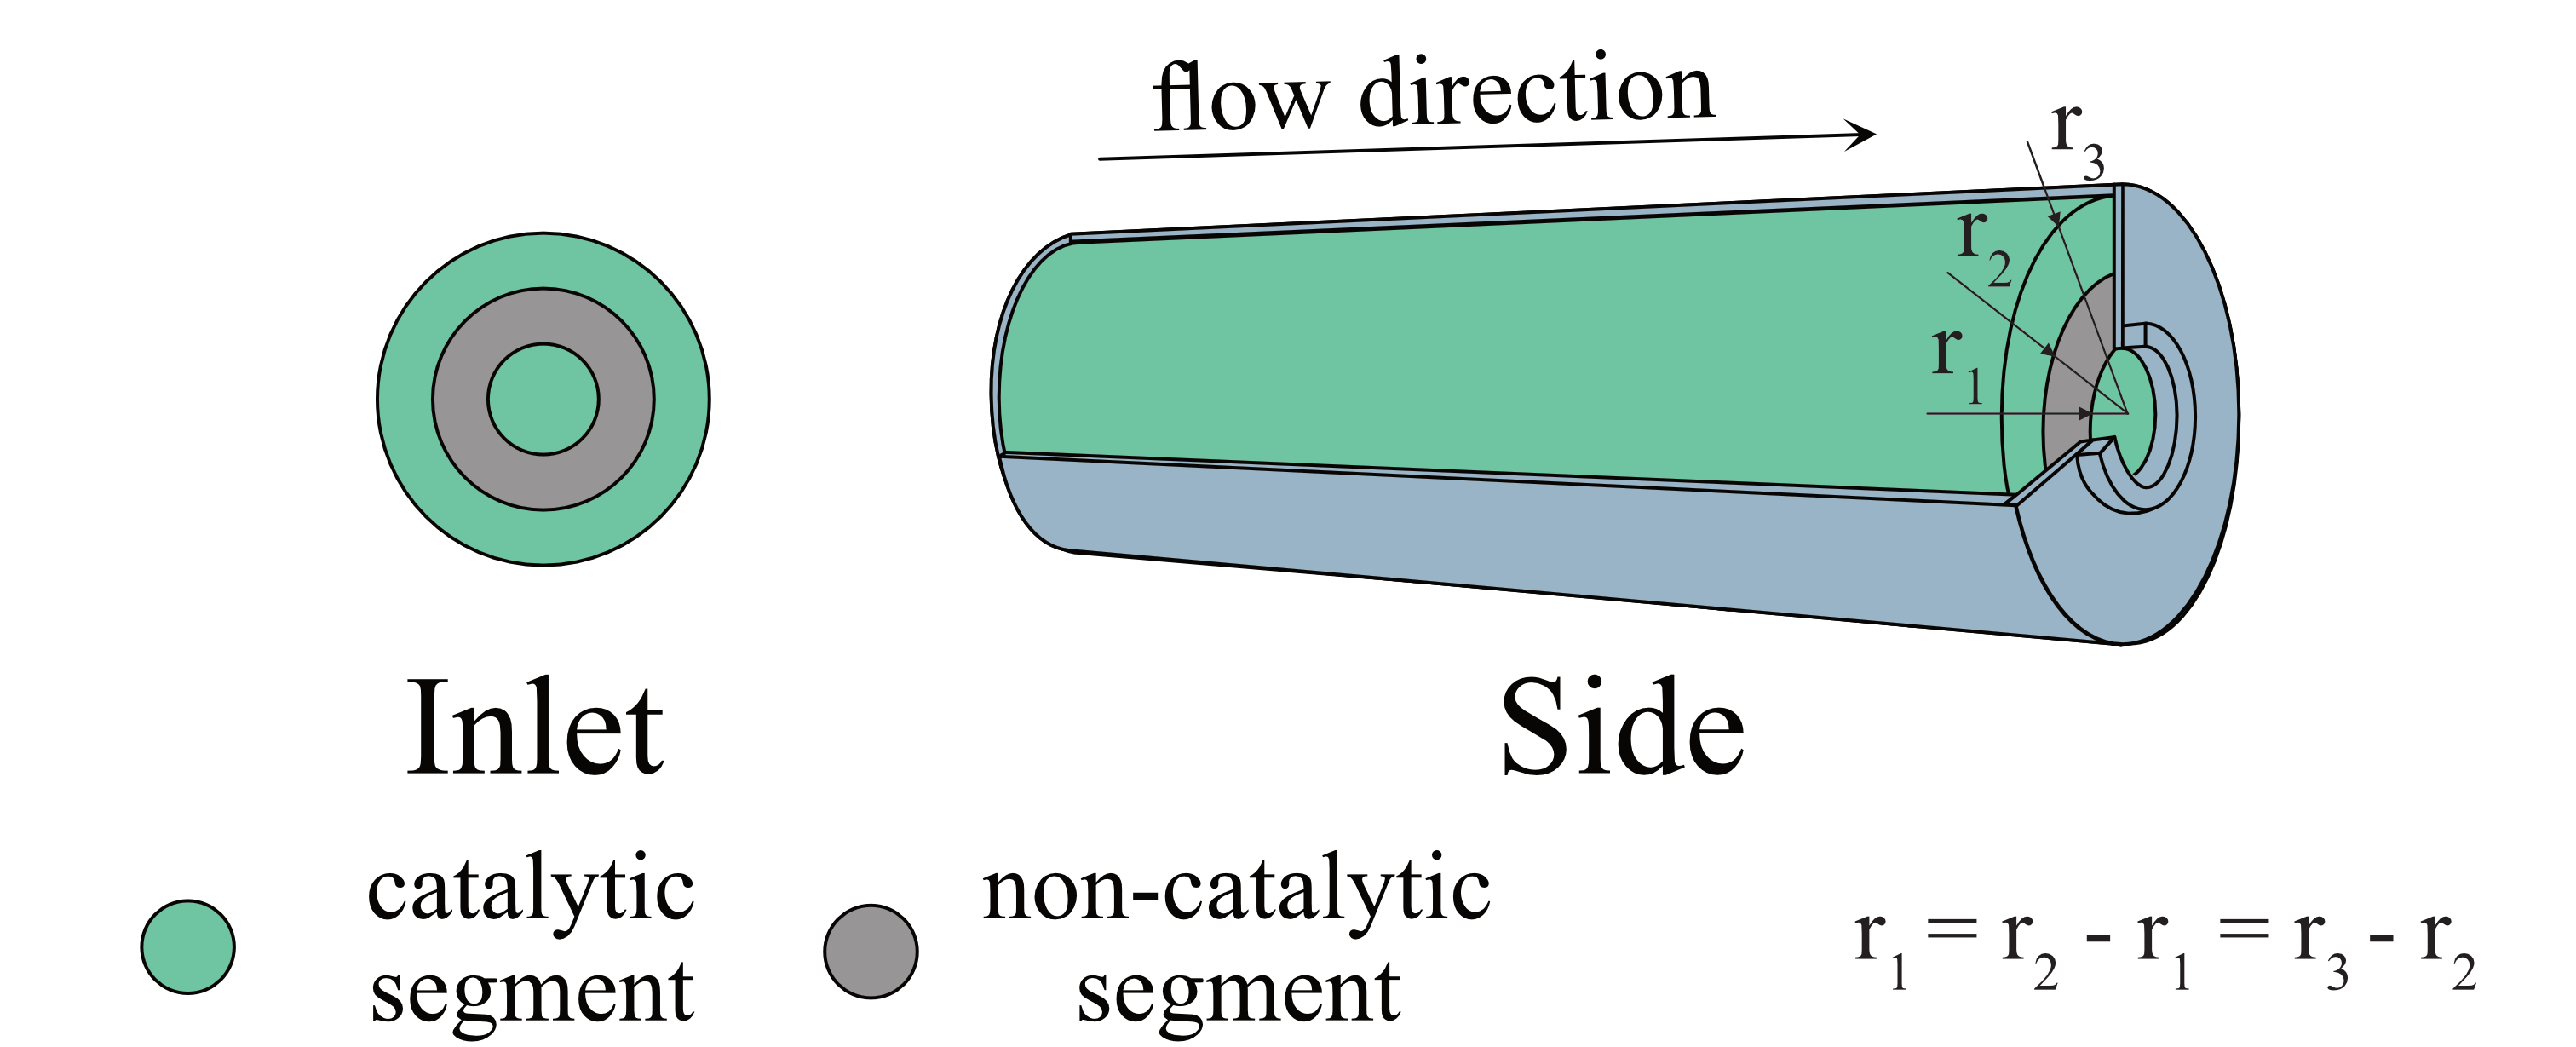
\includegraphics[width=120mm]{5seg.png}
%\caption{\label{fig:5seg}Catalytic insert division strategy I}
%\end{figure}
%
%
%\paragraph{Thermal fitness 80 \%, methane conversion 20 \%} \hspace{0pt} \\
%\noindent 
%
%\begin{figure}[h!]
%\centering
%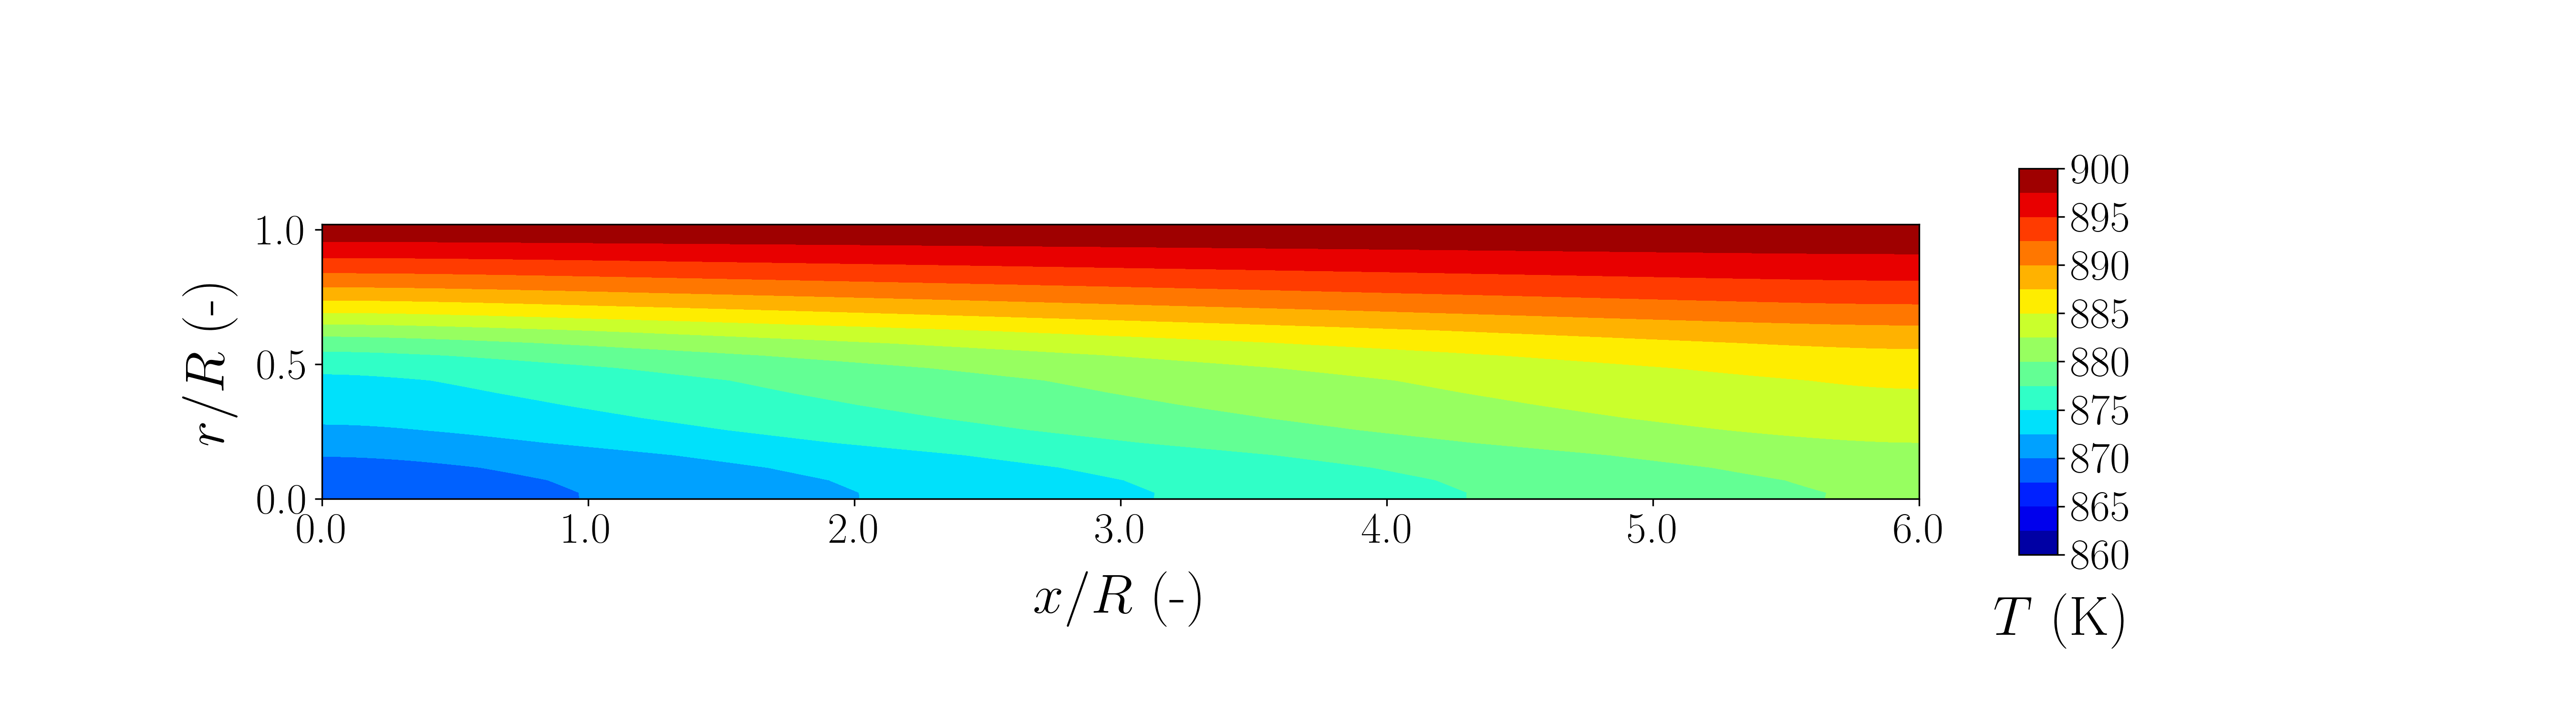
\includegraphics[width=190mm]{results/5/20C_80T/GEN1-TFIELD.png}
%\caption{\label{fig:5R2080G1-TField} Strategy I - Temperature field distribution - 1$^{\rm{st}}$ generation ($w_{\rm{CH_4}} = 0.2, w_T = 0.8$, $T_{\rm{in}}$ = 900 K, $u_{\rm{in}}$ = 0.15 m s$^{-1}$, $SC$ = 2.0)}
%\end{figure}
%
%\begin{figure}[h!]
%\centering
%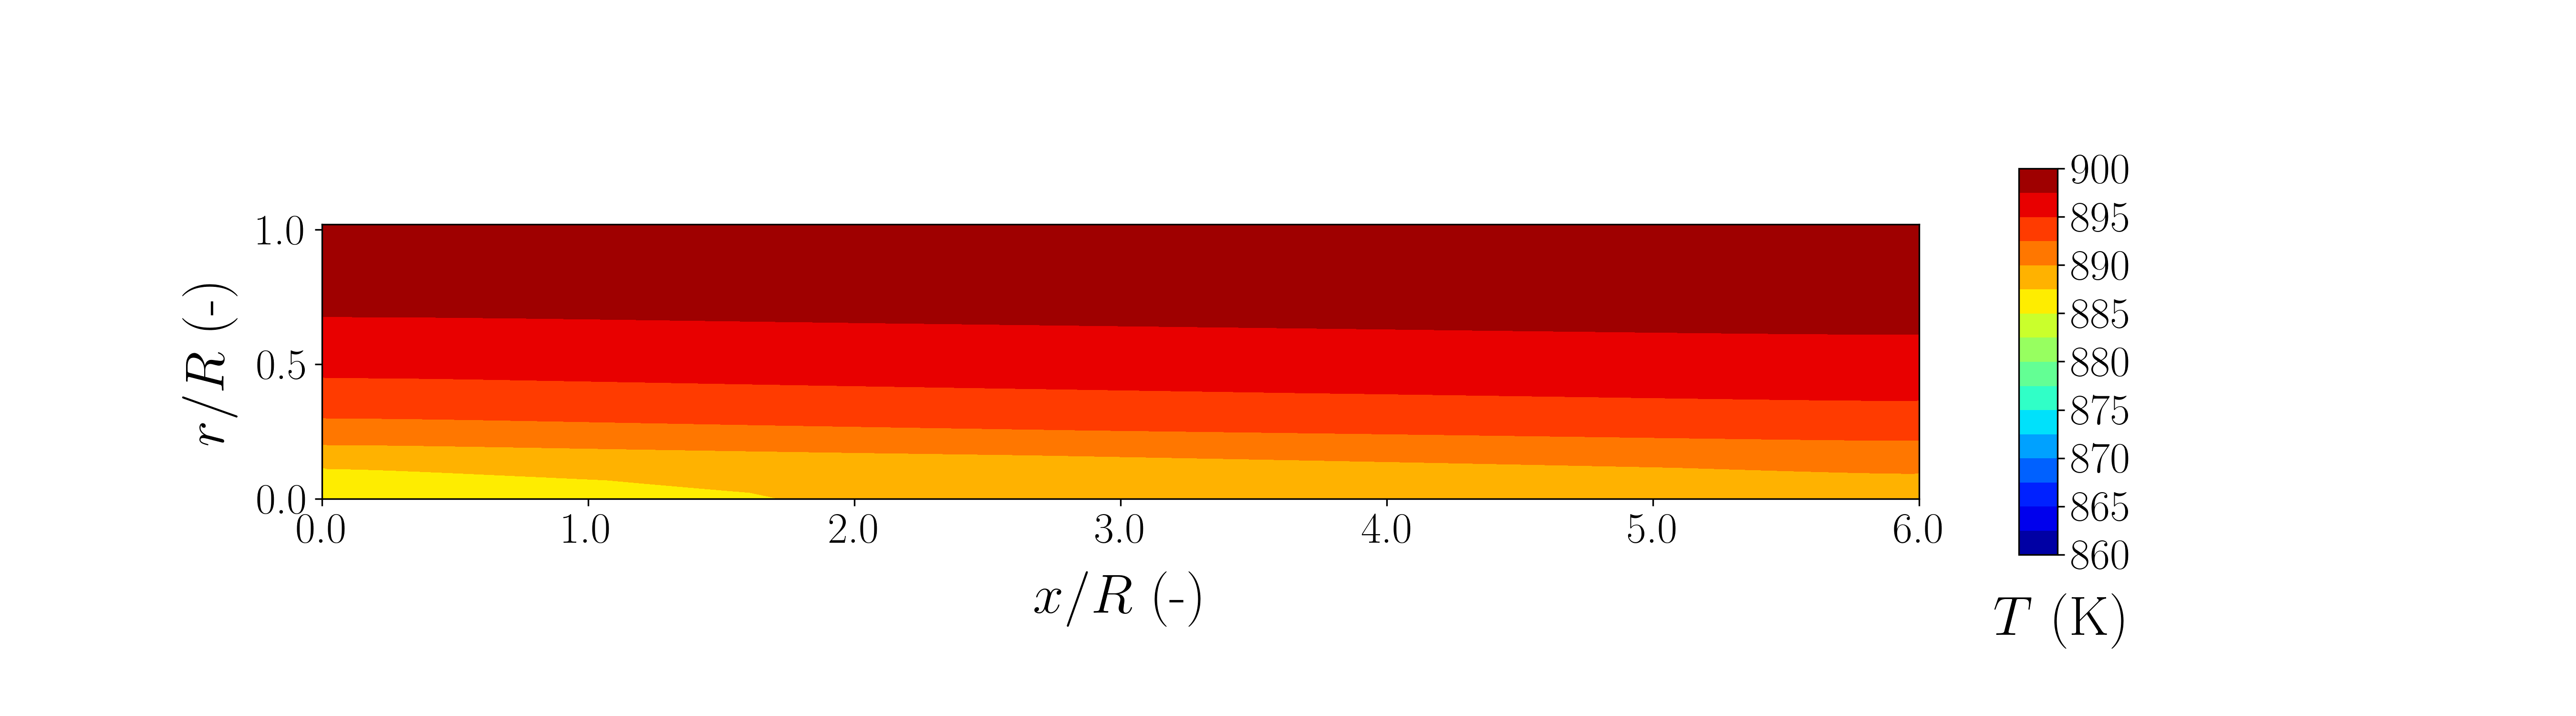
\includegraphics[width=190mm]{results/5/20C_80T/GEN15-TFIELD.png}
%\caption{\label{fig:5R2080G15-TField} Strategy I - Temperature field distribution - 15$^{\rm{th}}$ generation ($w_{\rm{CH_4}} = 0.2, w_T = 0.8$, $T_{\rm{in}}$ = 900 K, $u_{\rm{in}}$ = 0.15 m s$^{-1}$, $SC$ = 2.0)}
%\end{figure}
%
%\begin{figure}[h!]
%\centering
%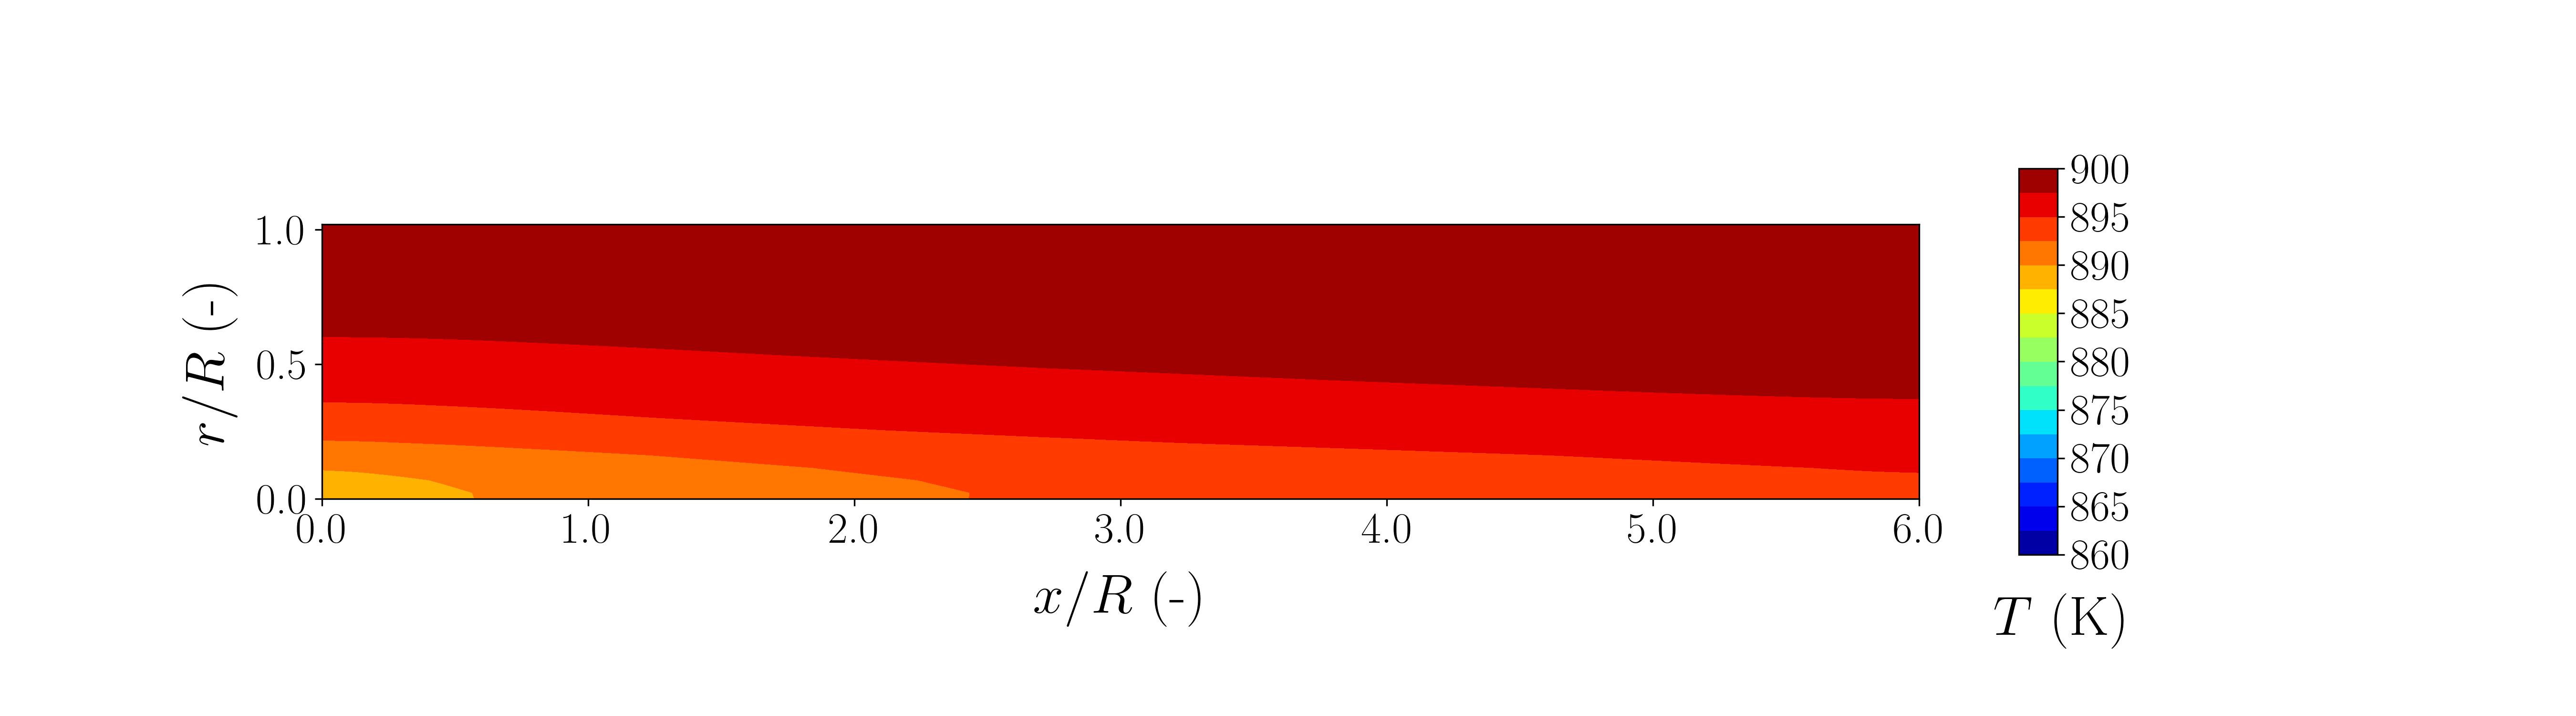
\includegraphics[width=190mm]{results/5/20C_80T/GEN30-TFIELD.png}
%\caption{\label{fig:5R2080G30-TField} Strategy I - Temperature field distribution - 30$^{\rm{th}}$ generation ($w_{\rm{CH_4}} = 0.2, w_T = 0.8$, $T_{\rm{in}}$ = 900 K, $u_{\rm{in}}$ = 0.15 m s$^{-1}$, $SC$ = 2.0)}
%\end{figure}
%
%
%\begin{figure}[h!]
%\centering
%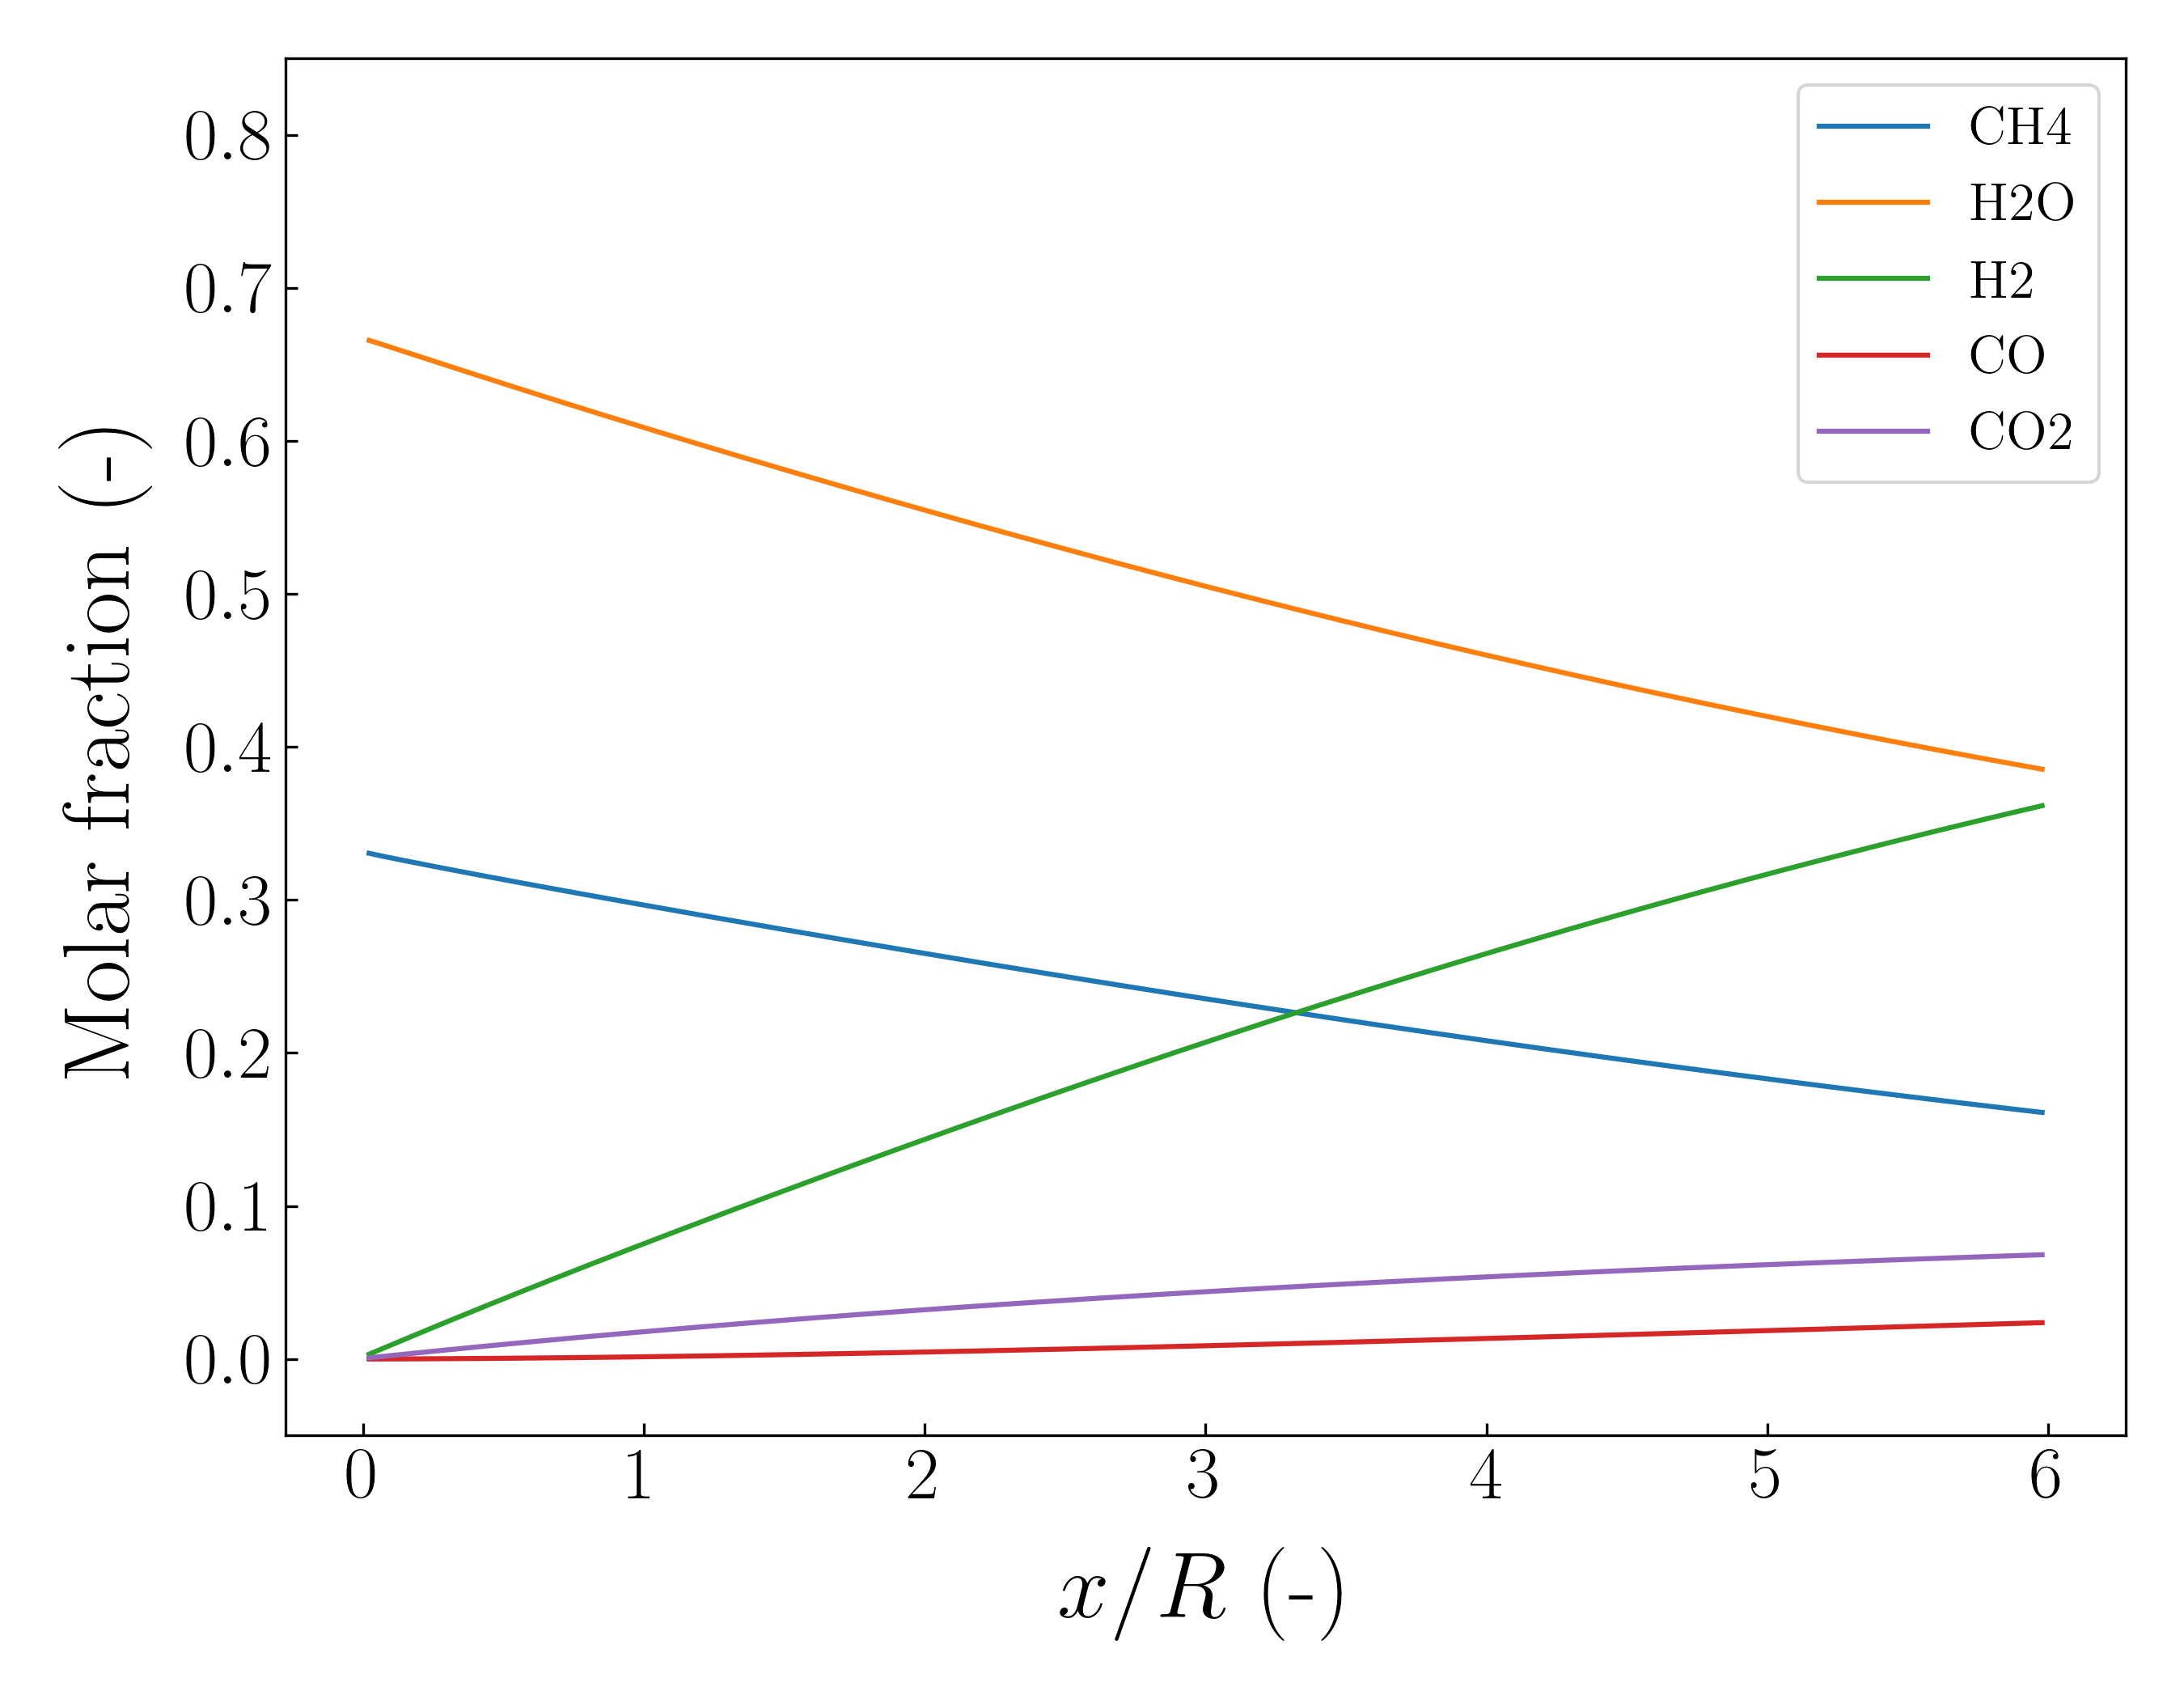
\includegraphics[width=80mm]{results/5/20C_80T/GEN1-AVG.png}
%\caption{\label{fig:5R2080G1-avg} Strategy I - Radius-averaged molar fractions - 1$^{\rm{st}}$ generation ($w_{\rm{CH_4}} = 0.2, w_T = 0.8$, $T_{\rm{in}}$ = 900 K, $u_{\rm{in}}$ = 0.15 m s$^{-1}$, $SC$ = 2.0)}
%\end{figure}
%
%\begin{figure}[h!]
%\centering
%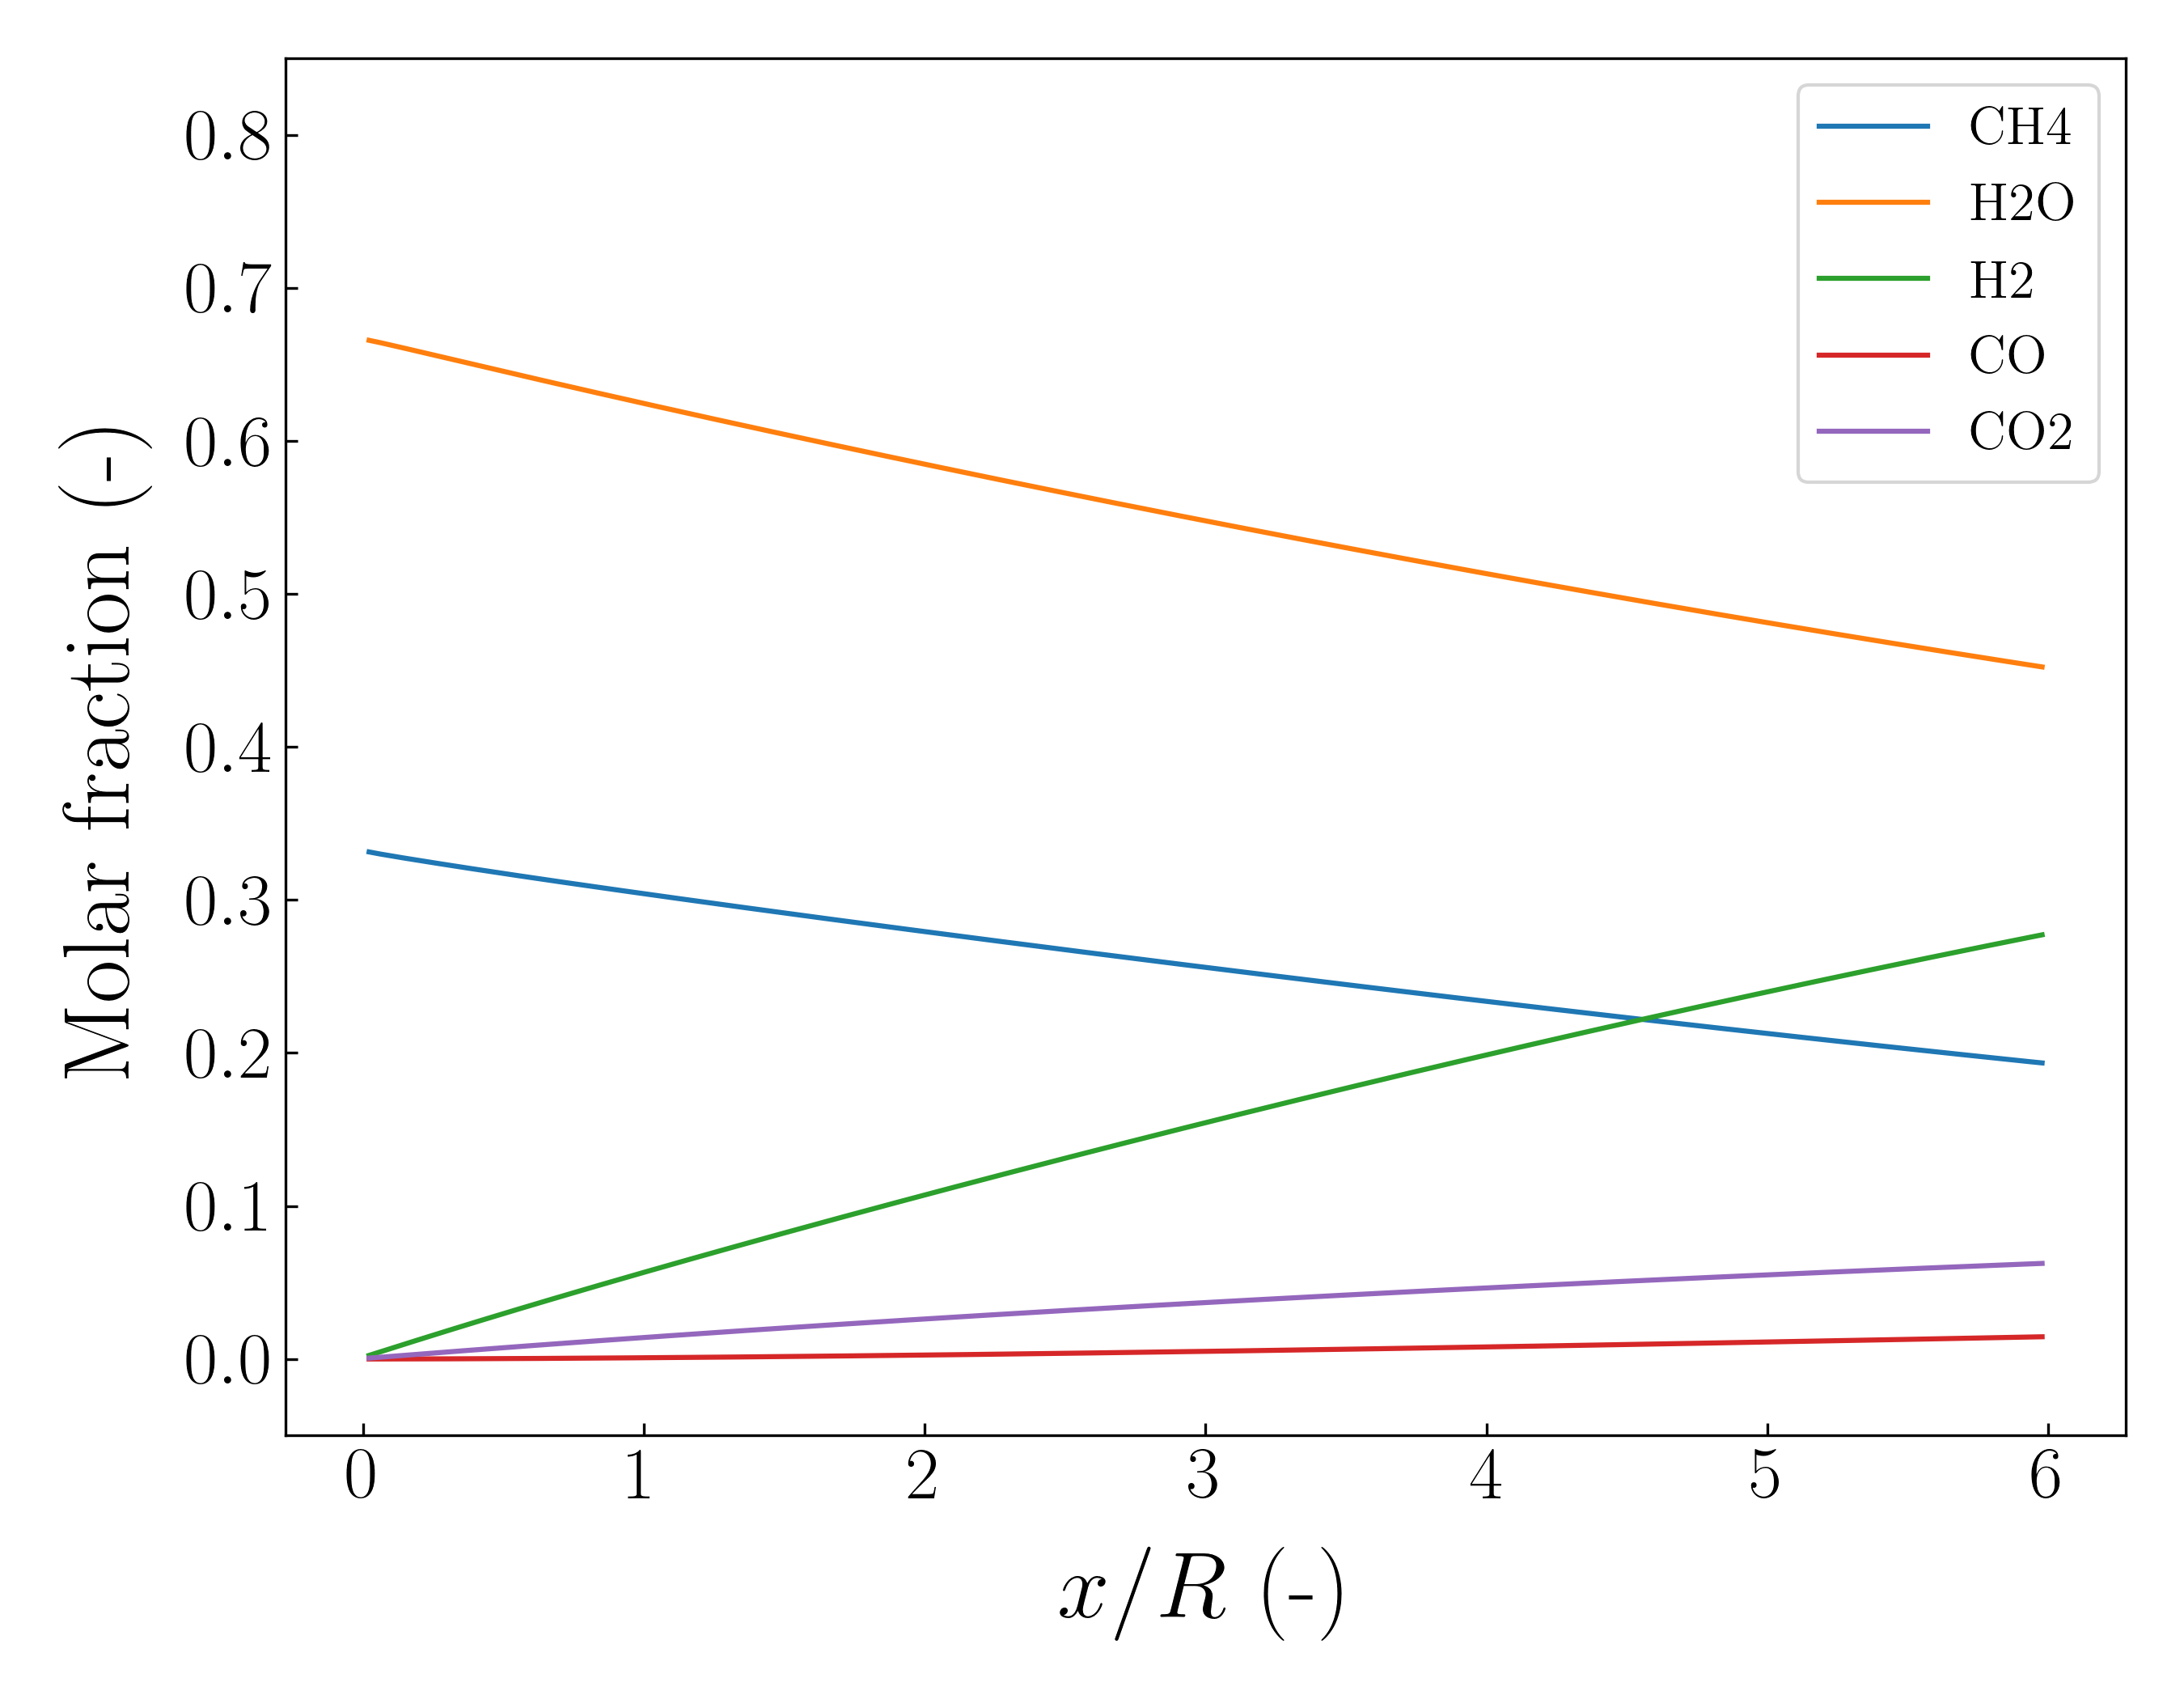
\includegraphics[width=80mm]{results/5/20C_80T/GEN15-AVG.png}
%\caption{\label{fig:5R2080G15-avg} Strategy I - Radius-averaged molar fractions - 15$^{\rm{th}}$ generation ($w_{\rm{CH_4}} = 0.2, w_T = 0.8$, $T_{\rm{in}}$ = 900 K, $u_{\rm{in}}$ = 0.15 m s$^{-1}$, $SC$ = 2.0)}
%\end{figure}
%
%\begin{figure}[h!]
%\centering
%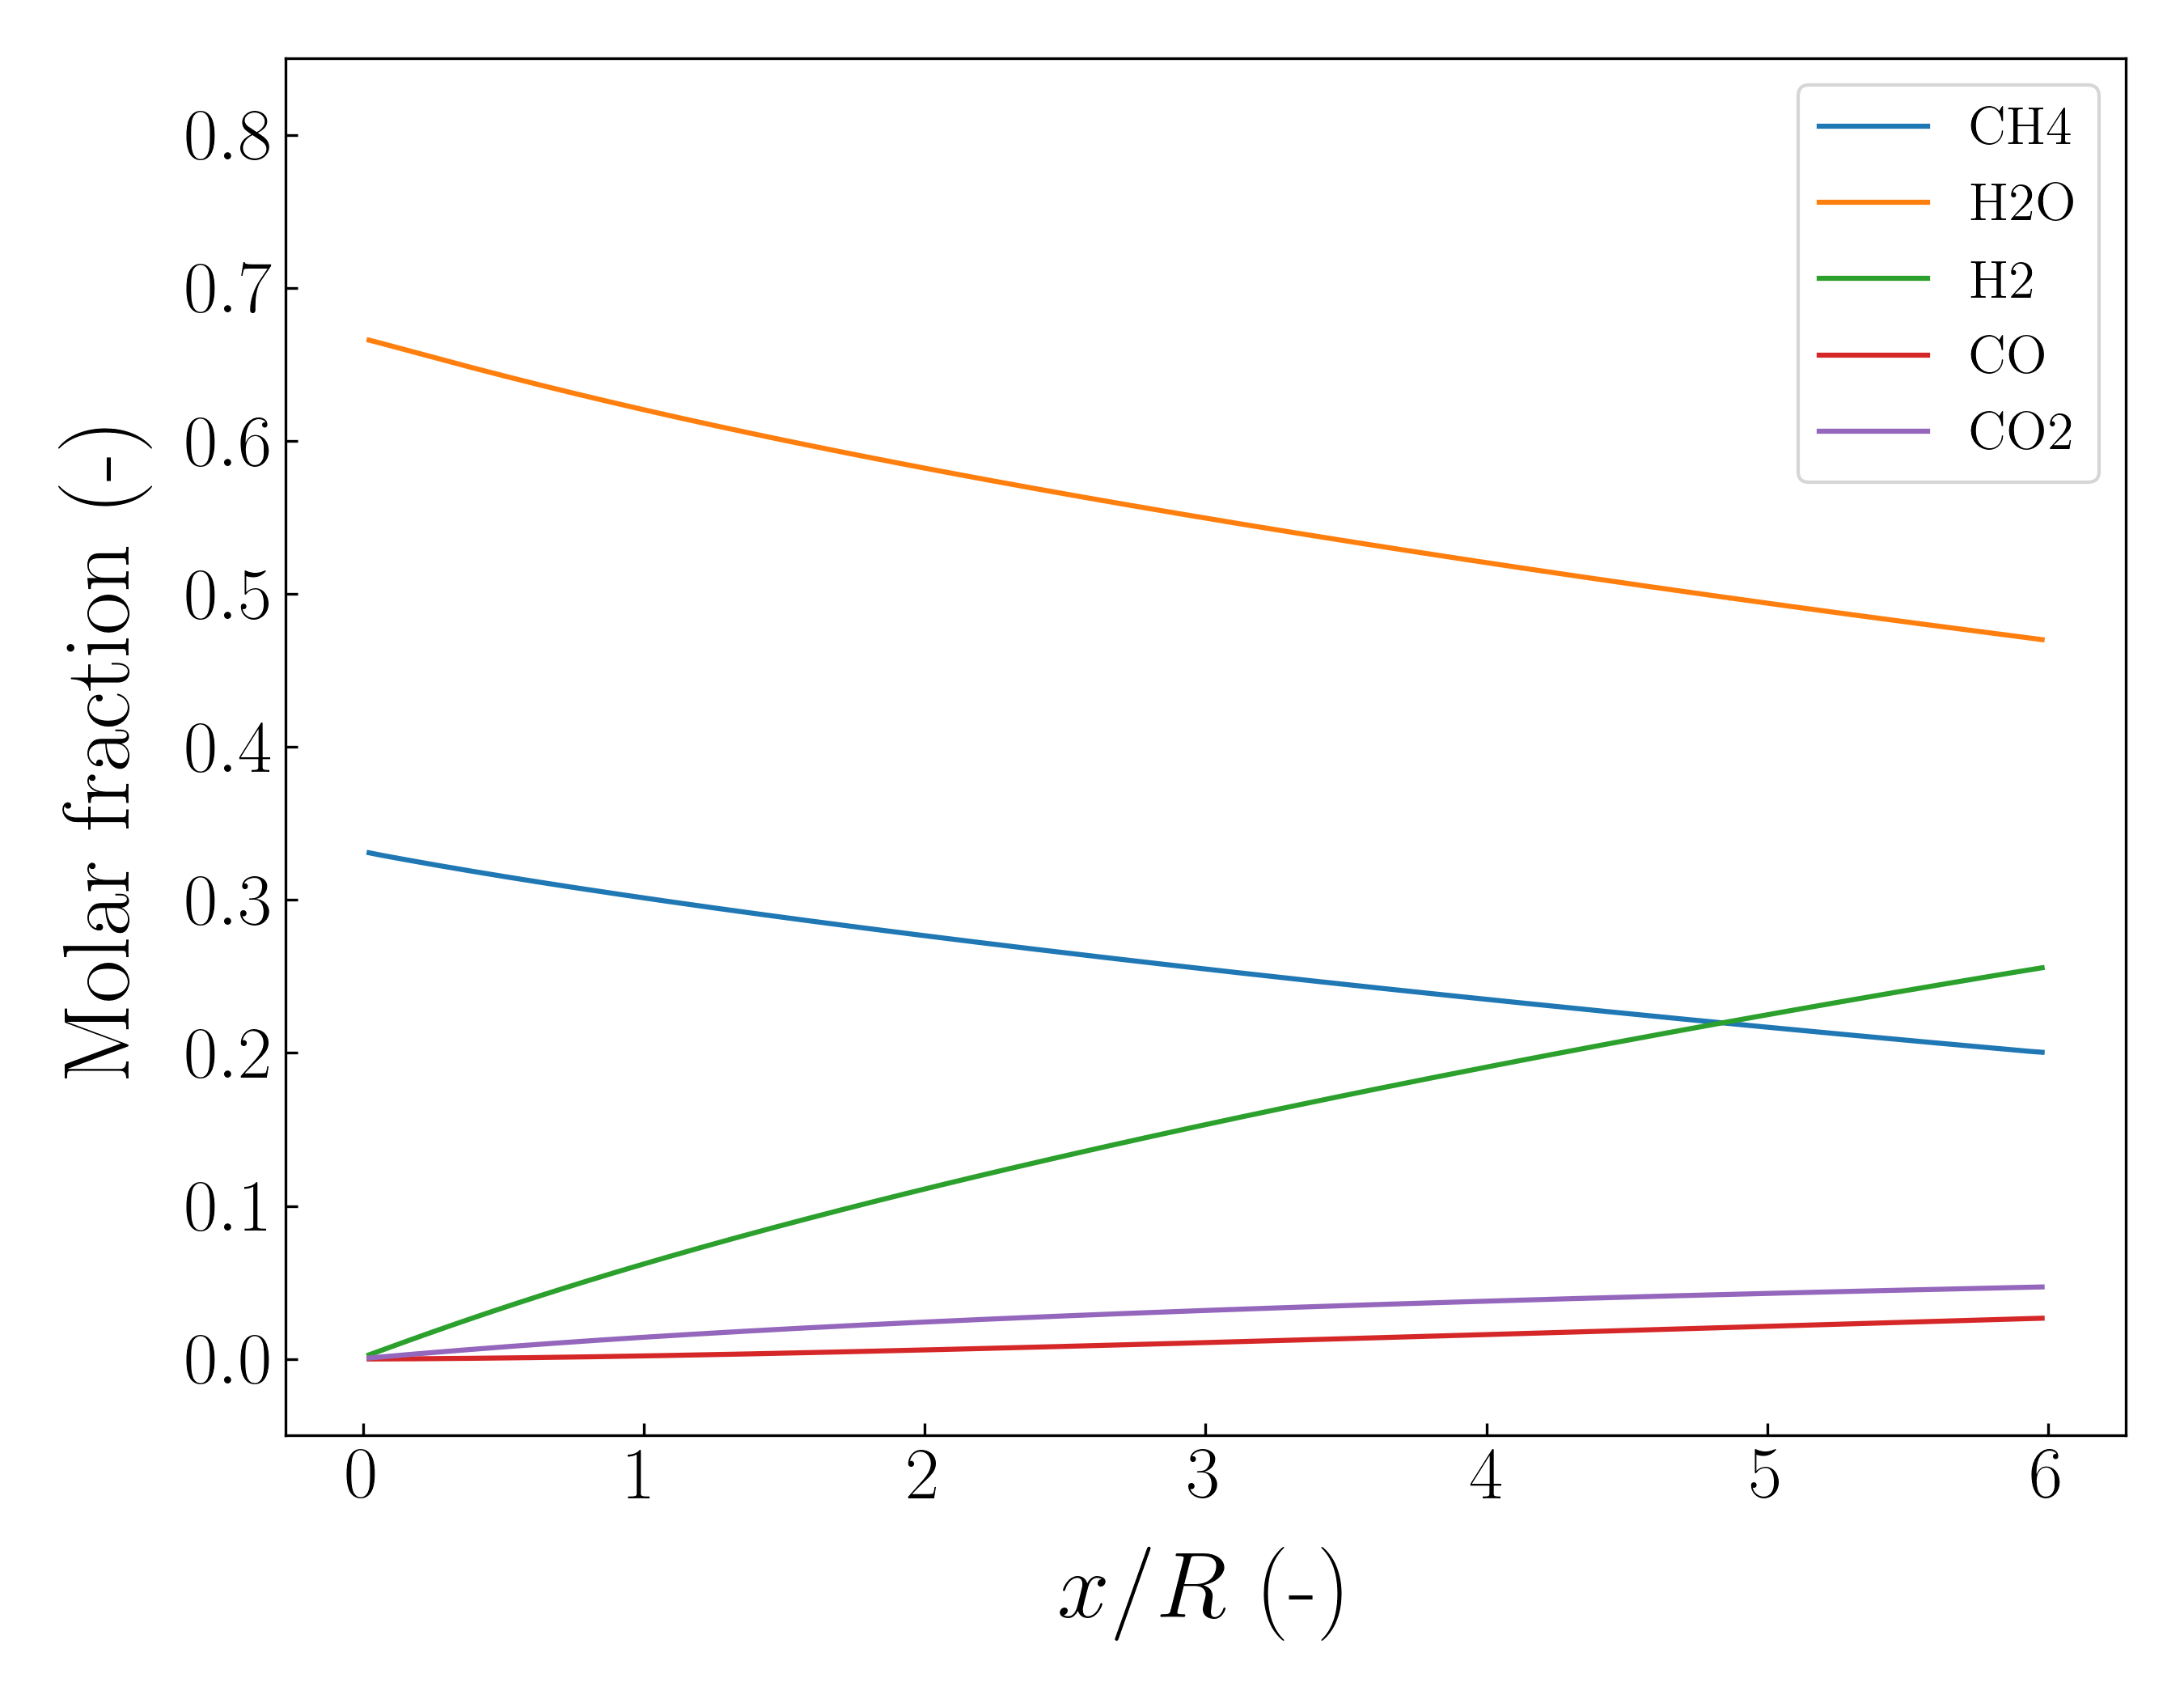
\includegraphics[width=80mm]{results/5/20C_80T/GEN30-AVG.png}
%\caption{\label{fig:5R2080G30-avg} Strategy I - Radius-averaged molar fractions -  30$^{\rm{th}}$ generation ($w_{\rm{CH_4}} = 0.2, w_T = 0.8$, $T_{\rm{in}}$ = 900 K, $u_{\rm{in}}$ = 0.15 m s$^{-1}$, $SC$ = 2.0)}
%\end{figure}
%
%\begin{figure}[h!]
%\centering
%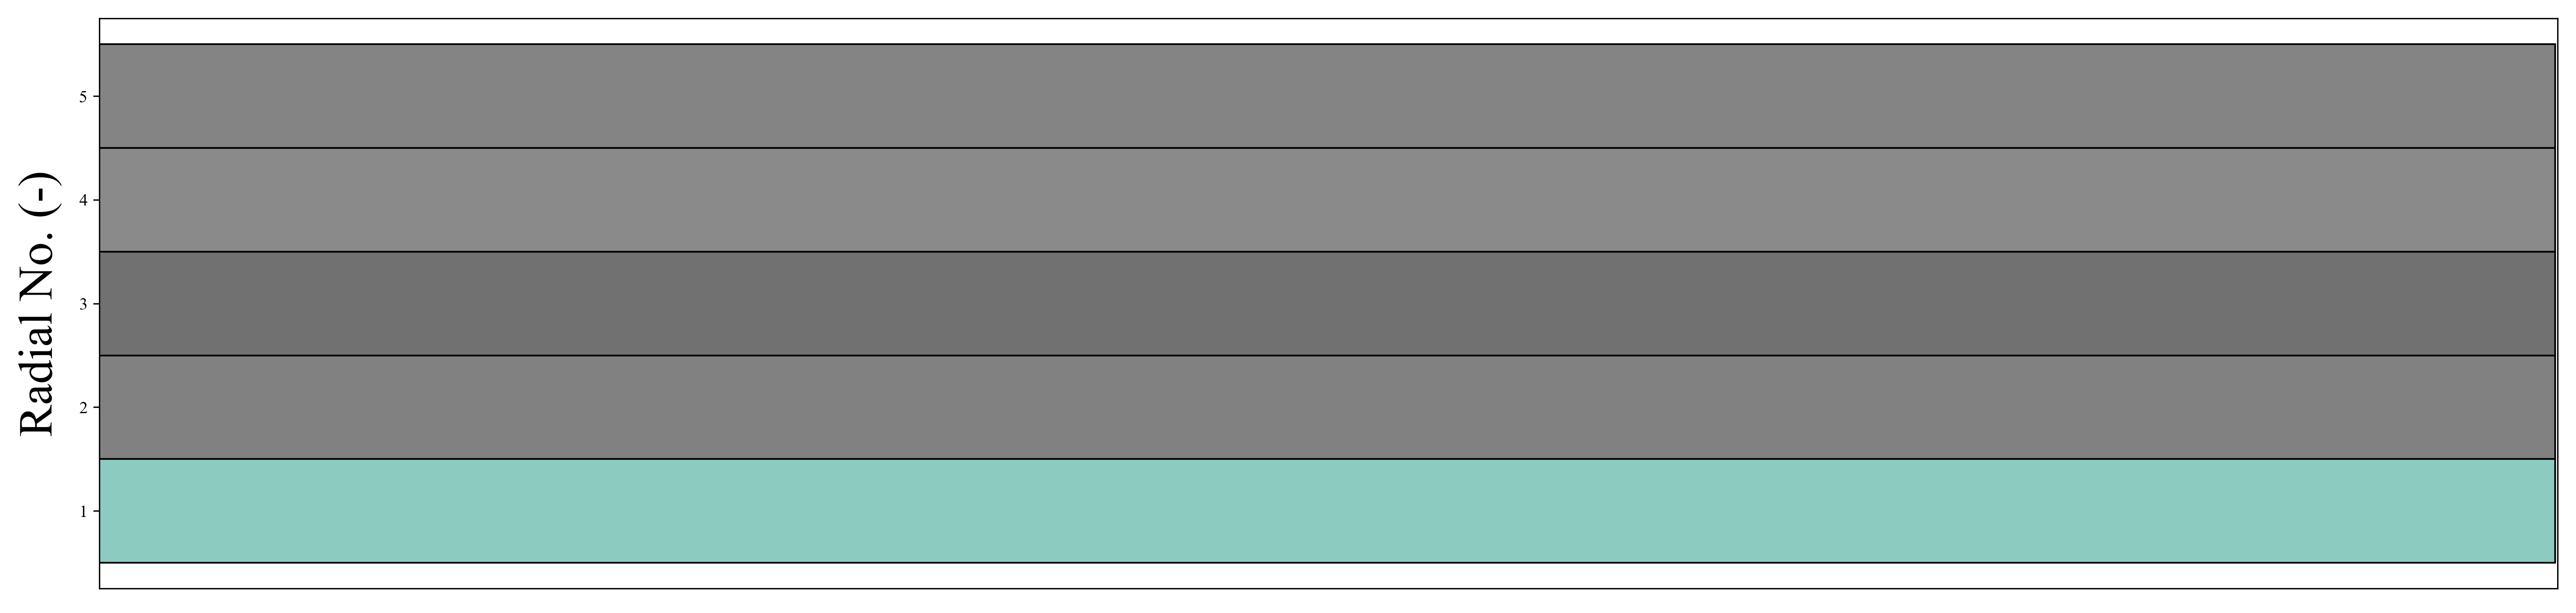
\includegraphics[width=120mm]{results/segments/5seg/20C80T/seg.png}
%\caption{\label{fig:30L6040G1-TField} Strategy I - Segments distribution for 30$^{\rm{th}}$ generation ($w_{\rm{CH_4}} = 0.2, w_T = 0.8$, $T_{\rm{in}}$ = 900 K, $u_{\rm{in}}$ = 0.15 m s$^{-1}$, $SC$ = 2.0)}
%\end{figure}
%
%\begin{figure}[h!]
%\centering
%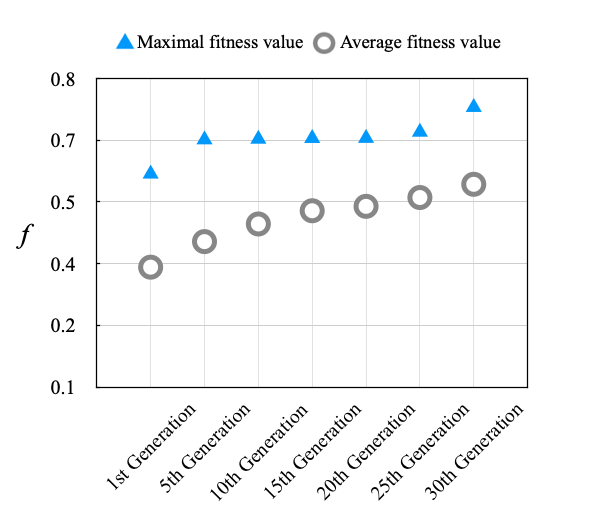
\includegraphics[width=100mm]{results/5/20C_80T.png}
%\caption{\label{fig:5R2080G-fitness} Strategy I - Fitness analysis throughout successive populations ($w_{\rm{CH_4}} = 0.2, w_T = 0.8$, $T_{\rm{in}}$ = 900 K, $u_{\rm{in}}$ = 0.15 m s$^{-1}$, $SC$ = 2.0)}
%\end{figure}
%
%
%
%\clearpage
%
%
%
%\paragraph{Thermal fitness 60 \%, methane conversion 40 \%} \hspace{0pt} \\
%\noindent 
%
%
%\begin{figure}[h!]
%\centering
%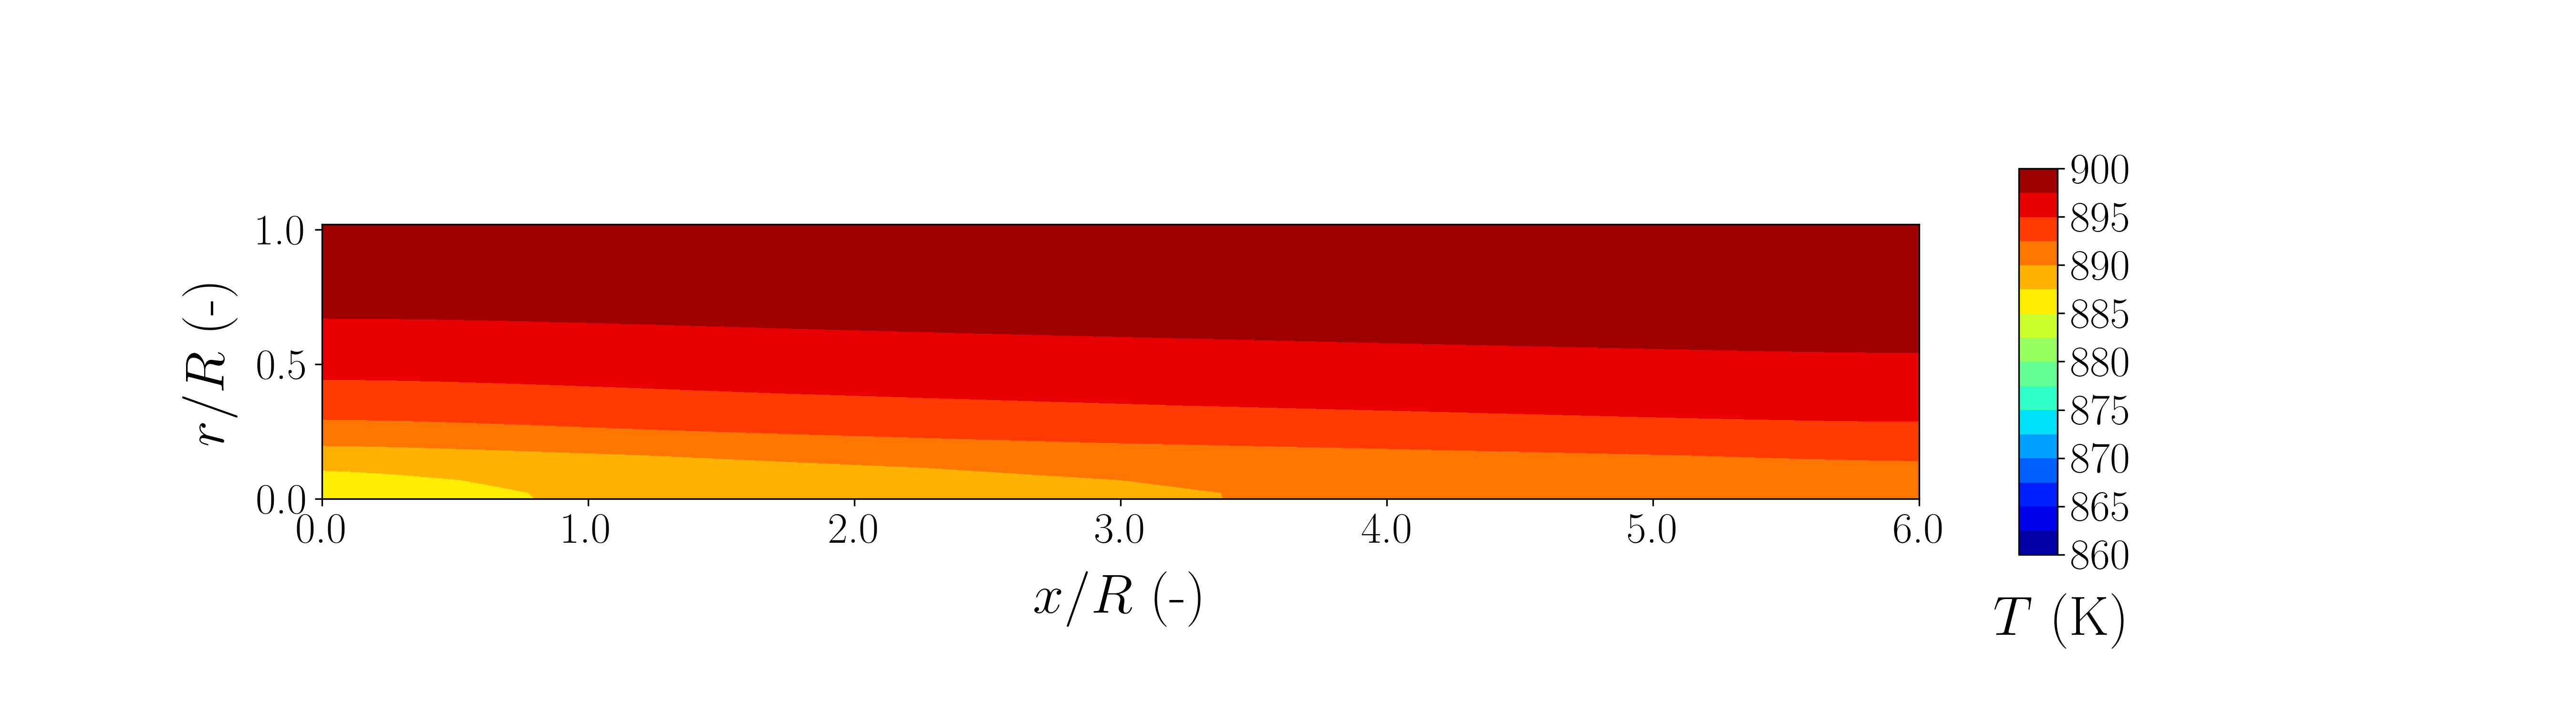
\includegraphics[width=190mm]{results/5/40C_60T/GEN1-TFIELD.png}
%\caption{\label{fig:5R4060G1-TField} Strategy I - Temperature field distribution - 1$^{\rm{st}}$ generation ($w_{\rm{CH_4}} = 0.4, w_T = 0.6$, $T_{\rm{in}}$ = 900 K, $u_{\rm{in}}$ = 0.15 m s$^{-1}$, $SC$ = 2.0)}
%\end{figure}
%
%\begin{figure}[h!]
%\centering
%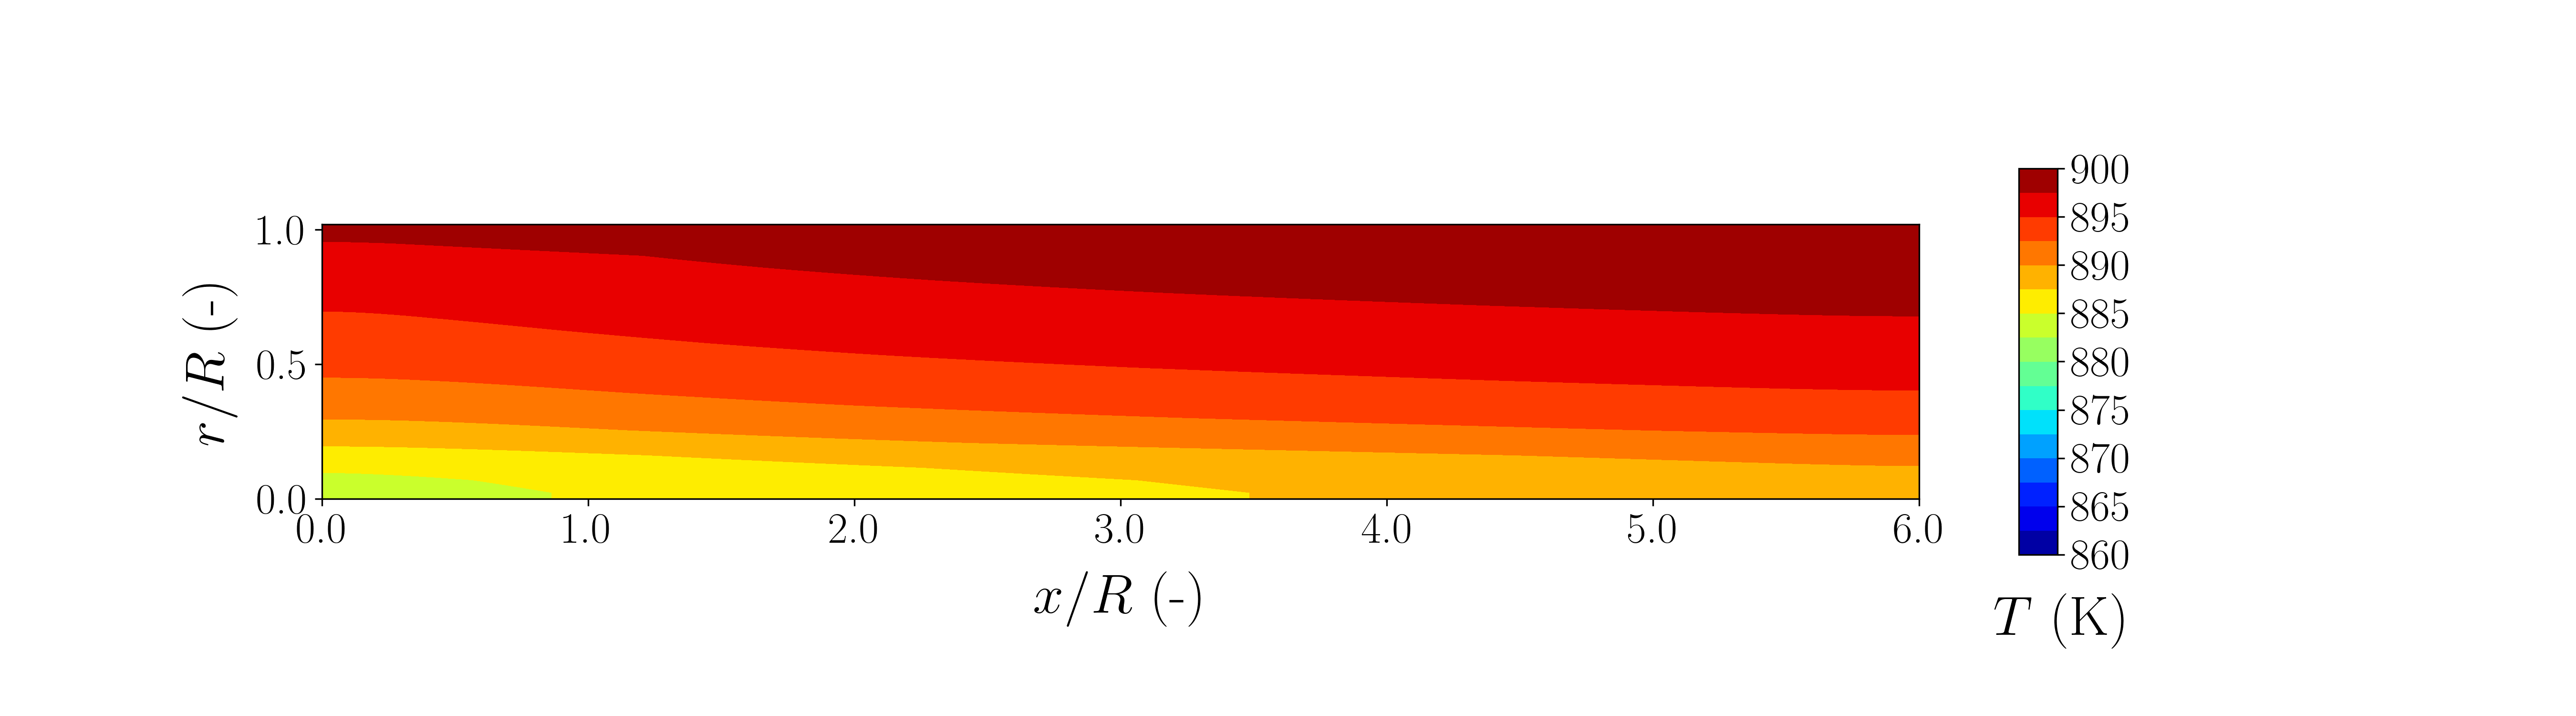
\includegraphics[width=190mm]{results/5/40C_60T/GEN15-TFIELD.png}
%\caption{\label{fig:5R4060G15-TField} Strategy I - Temperature field distribution - 15$^{\rm{th}}$ generation ($w_{\rm{CH_4}} = 0.4, w_T = 0.6$, $T_{\rm{in}}$ = 900 K, $u_{\rm{in}}$ = 0.15 m s$^{-1}$, $SC$ = 2.0)}
%\end{figure}
%
%\begin{figure}[h!]
%\centering
%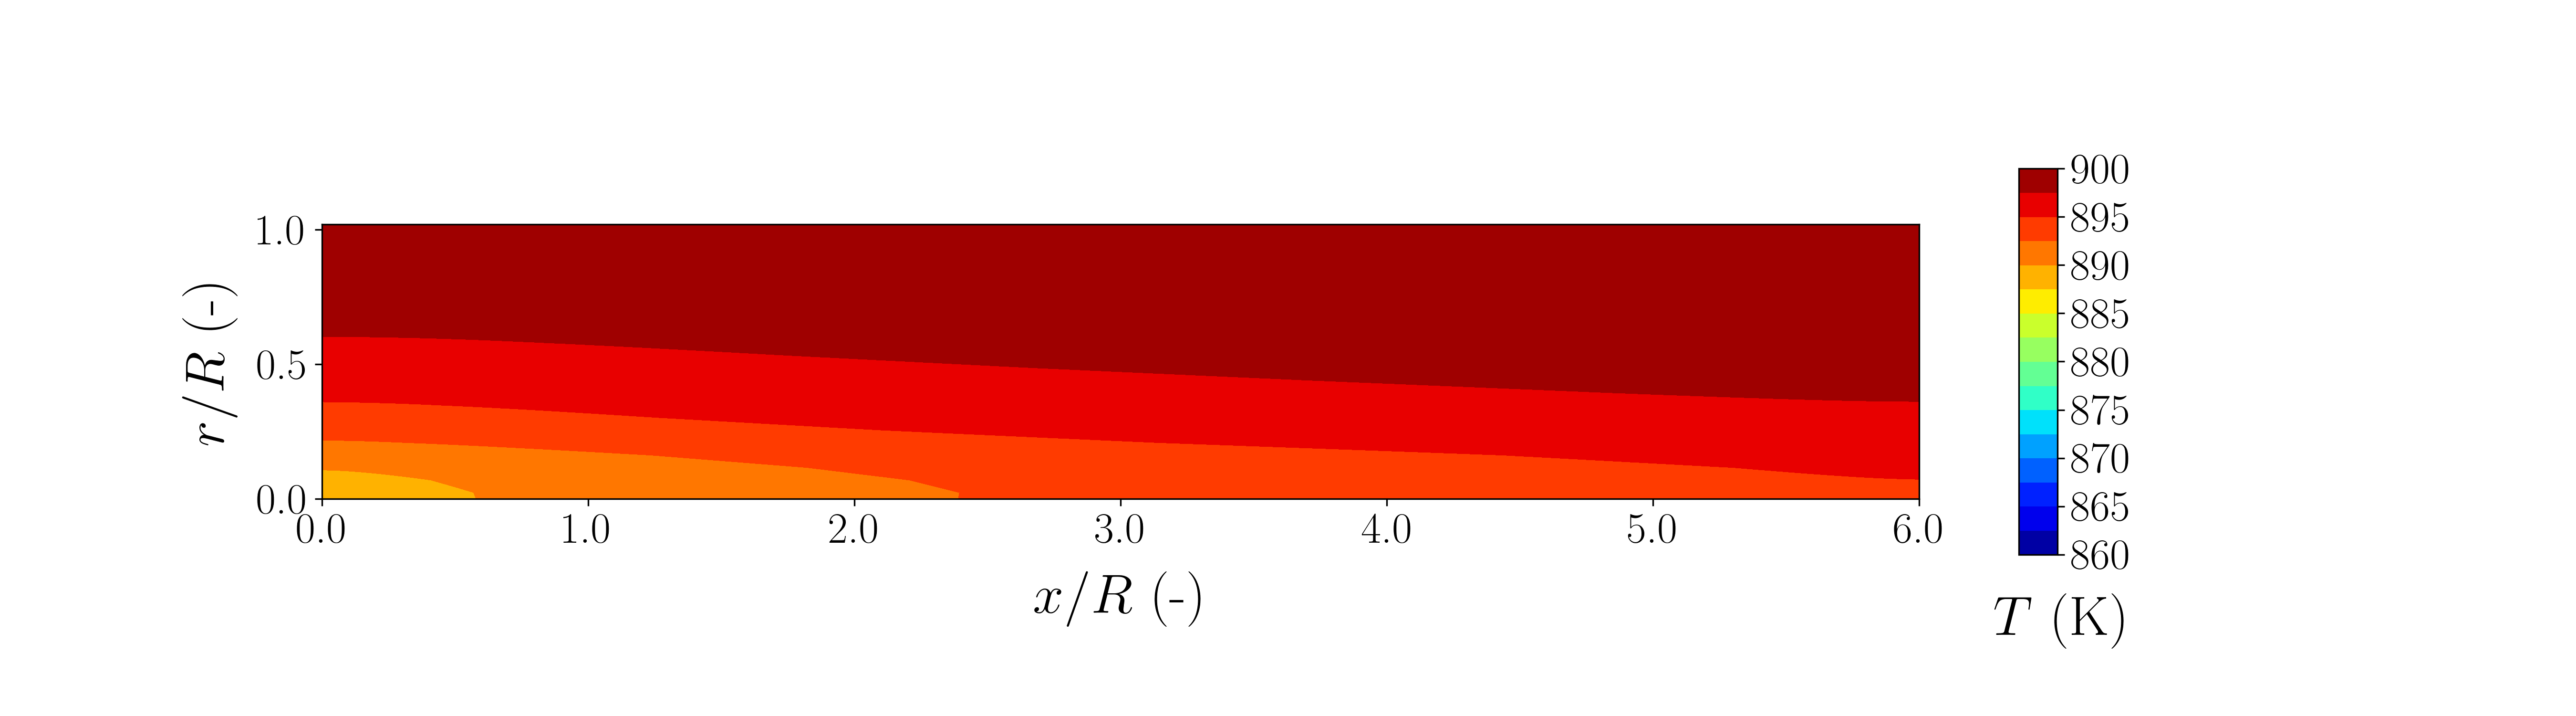
\includegraphics[width=190mm]{results/5/40C_60T/GEN30-TFIELD.png}
%\caption{\label{fig:5R4060G30-TField} Strategy I - Temperature field distribution - 30$^{\rm{th}}$ generation ($w_{\rm{CH_4}} = 0.4, w_T = 0.6$, $T_{\rm{in}}$ = 900 K, $u_{\rm{in}}$ = 0.15 m s$^{-1}$, $SC$ = 2.0)}
%\end{figure}
%
%
%\begin{figure}[h!]
%\centering
%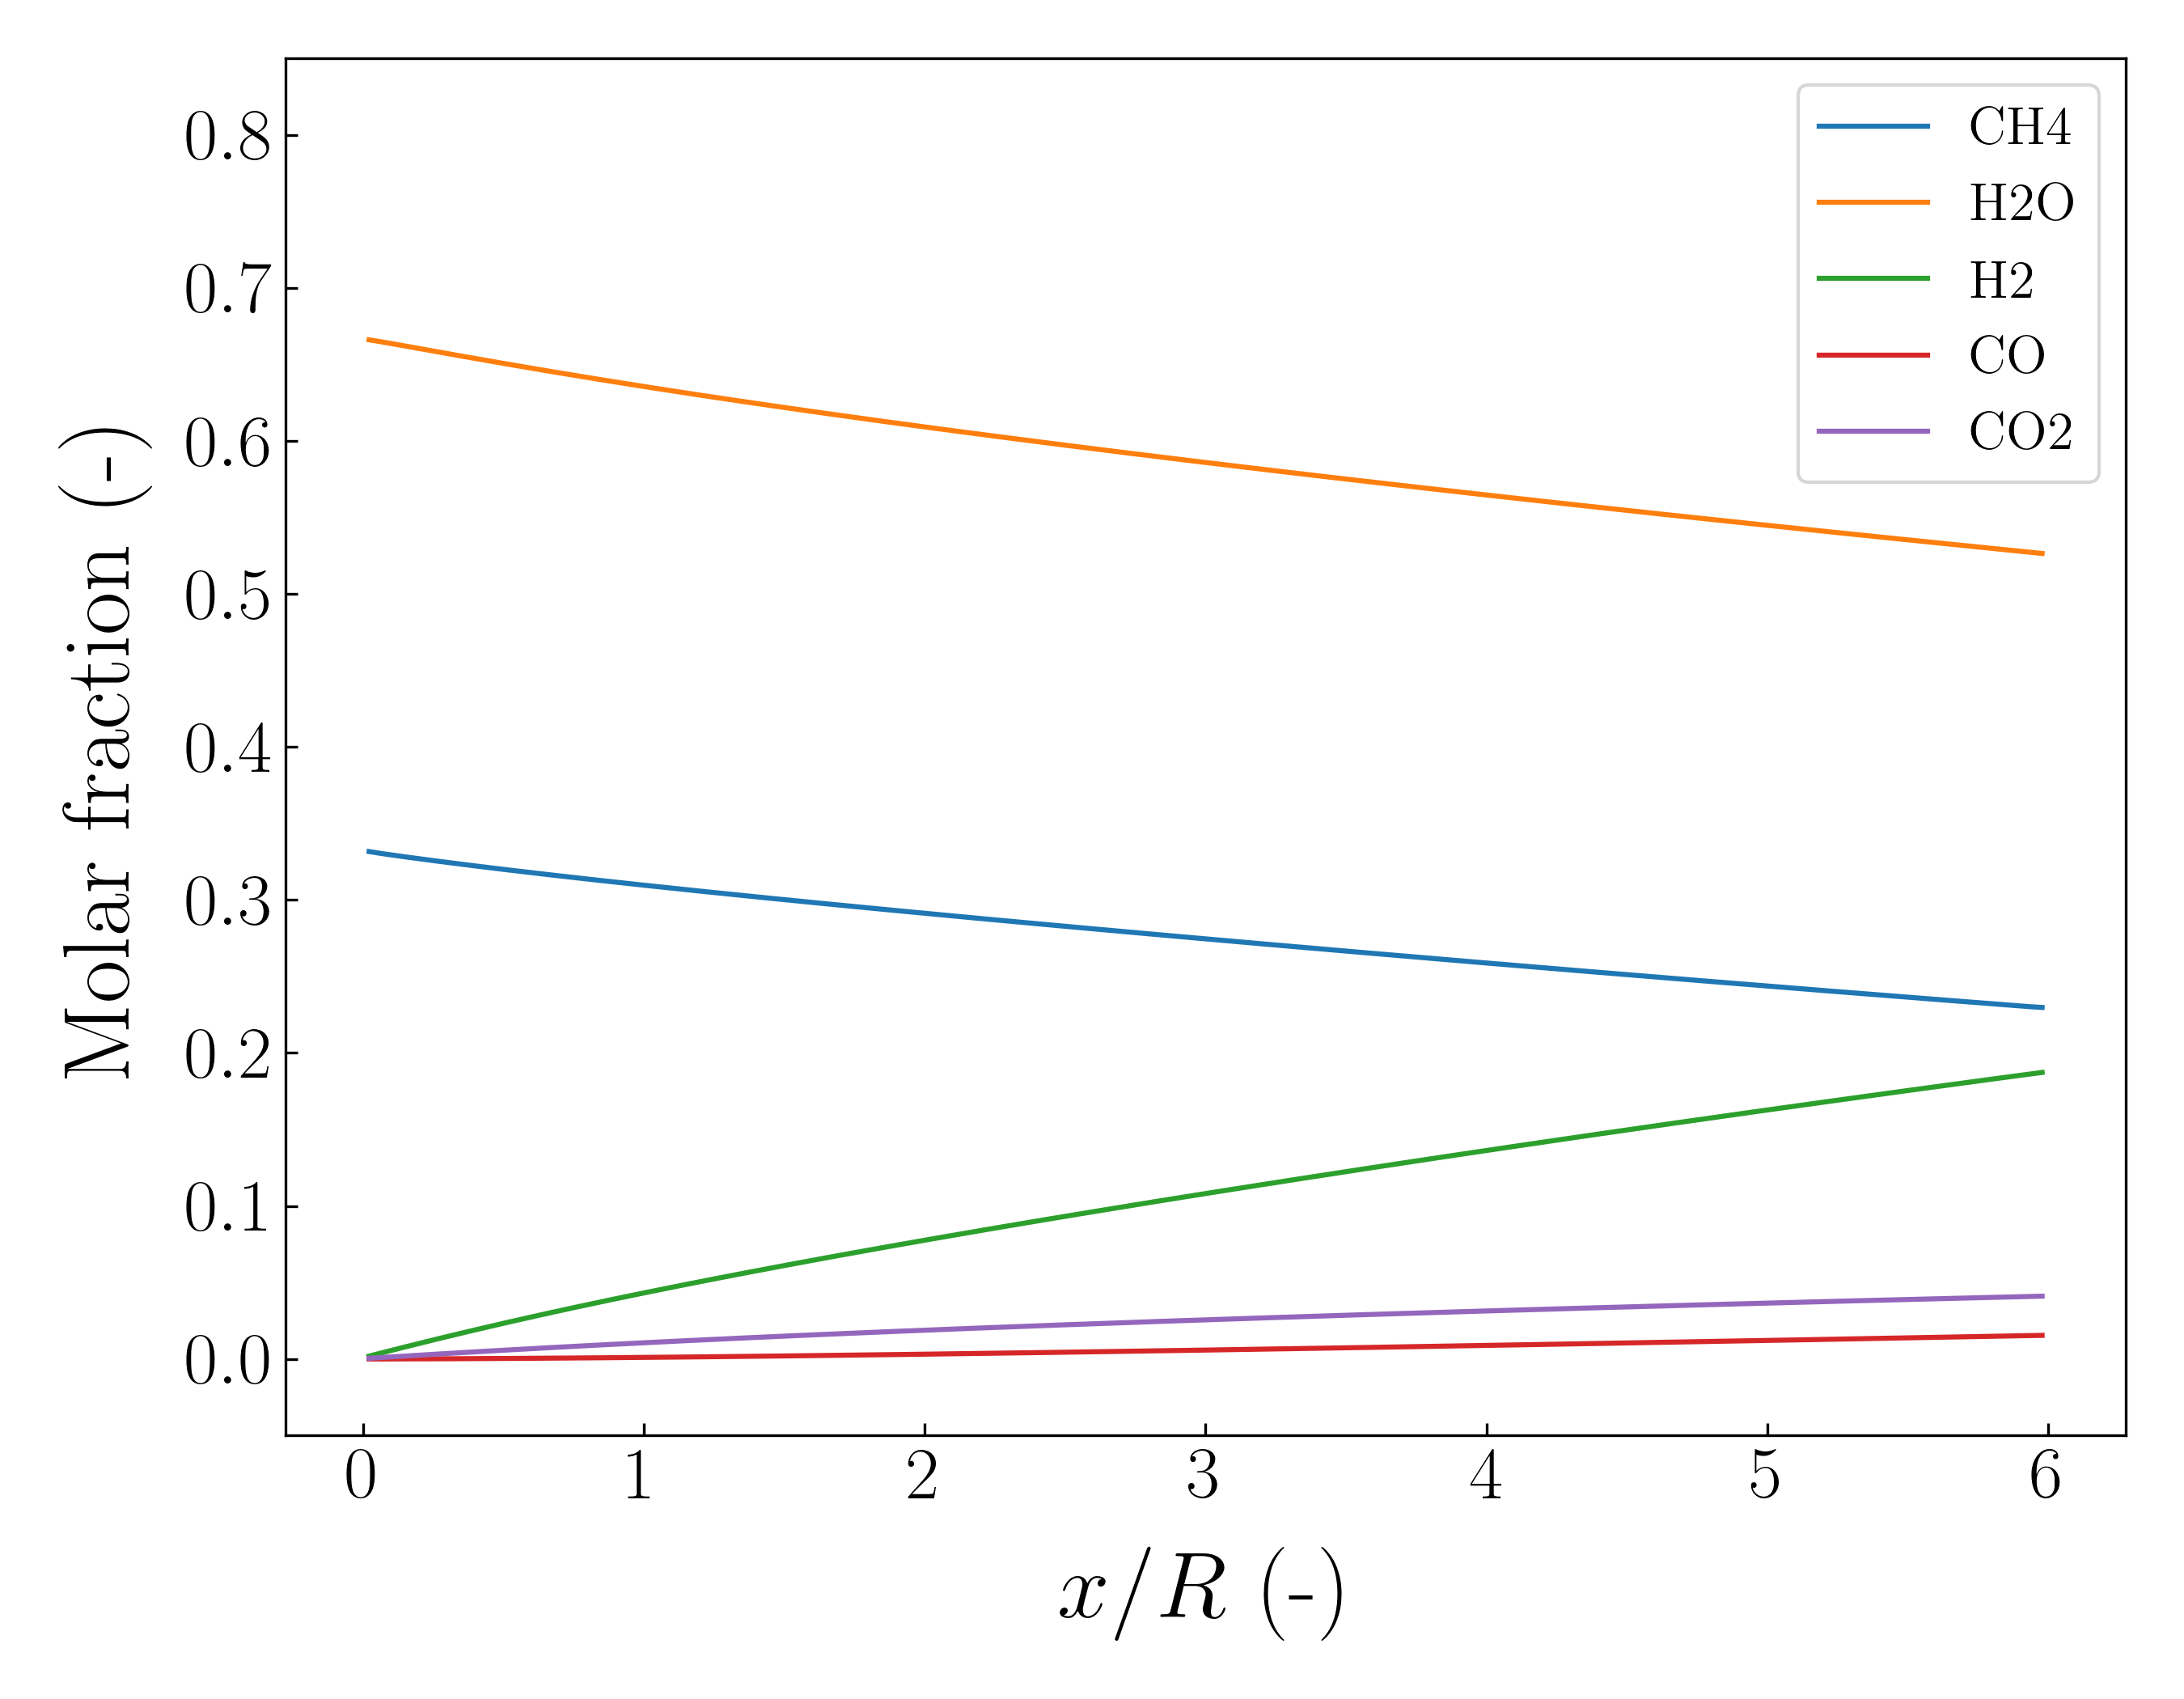
\includegraphics[width=80mm]{results/5/40C_60T/GEN1-AVG.png}
%\caption{\label{fig:5R4060G1-avg} Strategy I - Radius-averaged molar fractions - 1$^{\rm{st}}$ generation ($w_{\rm{CH_4}} = 0.4, w_T = 0.6$, $T_{\rm{in}}$ = 900 K, $u_{\rm{in}}$ = 0.15 m s$^{-1}$, $SC$ = 2.0)}
%\end{figure}
%
%\begin{figure}[h!]
%\centering
%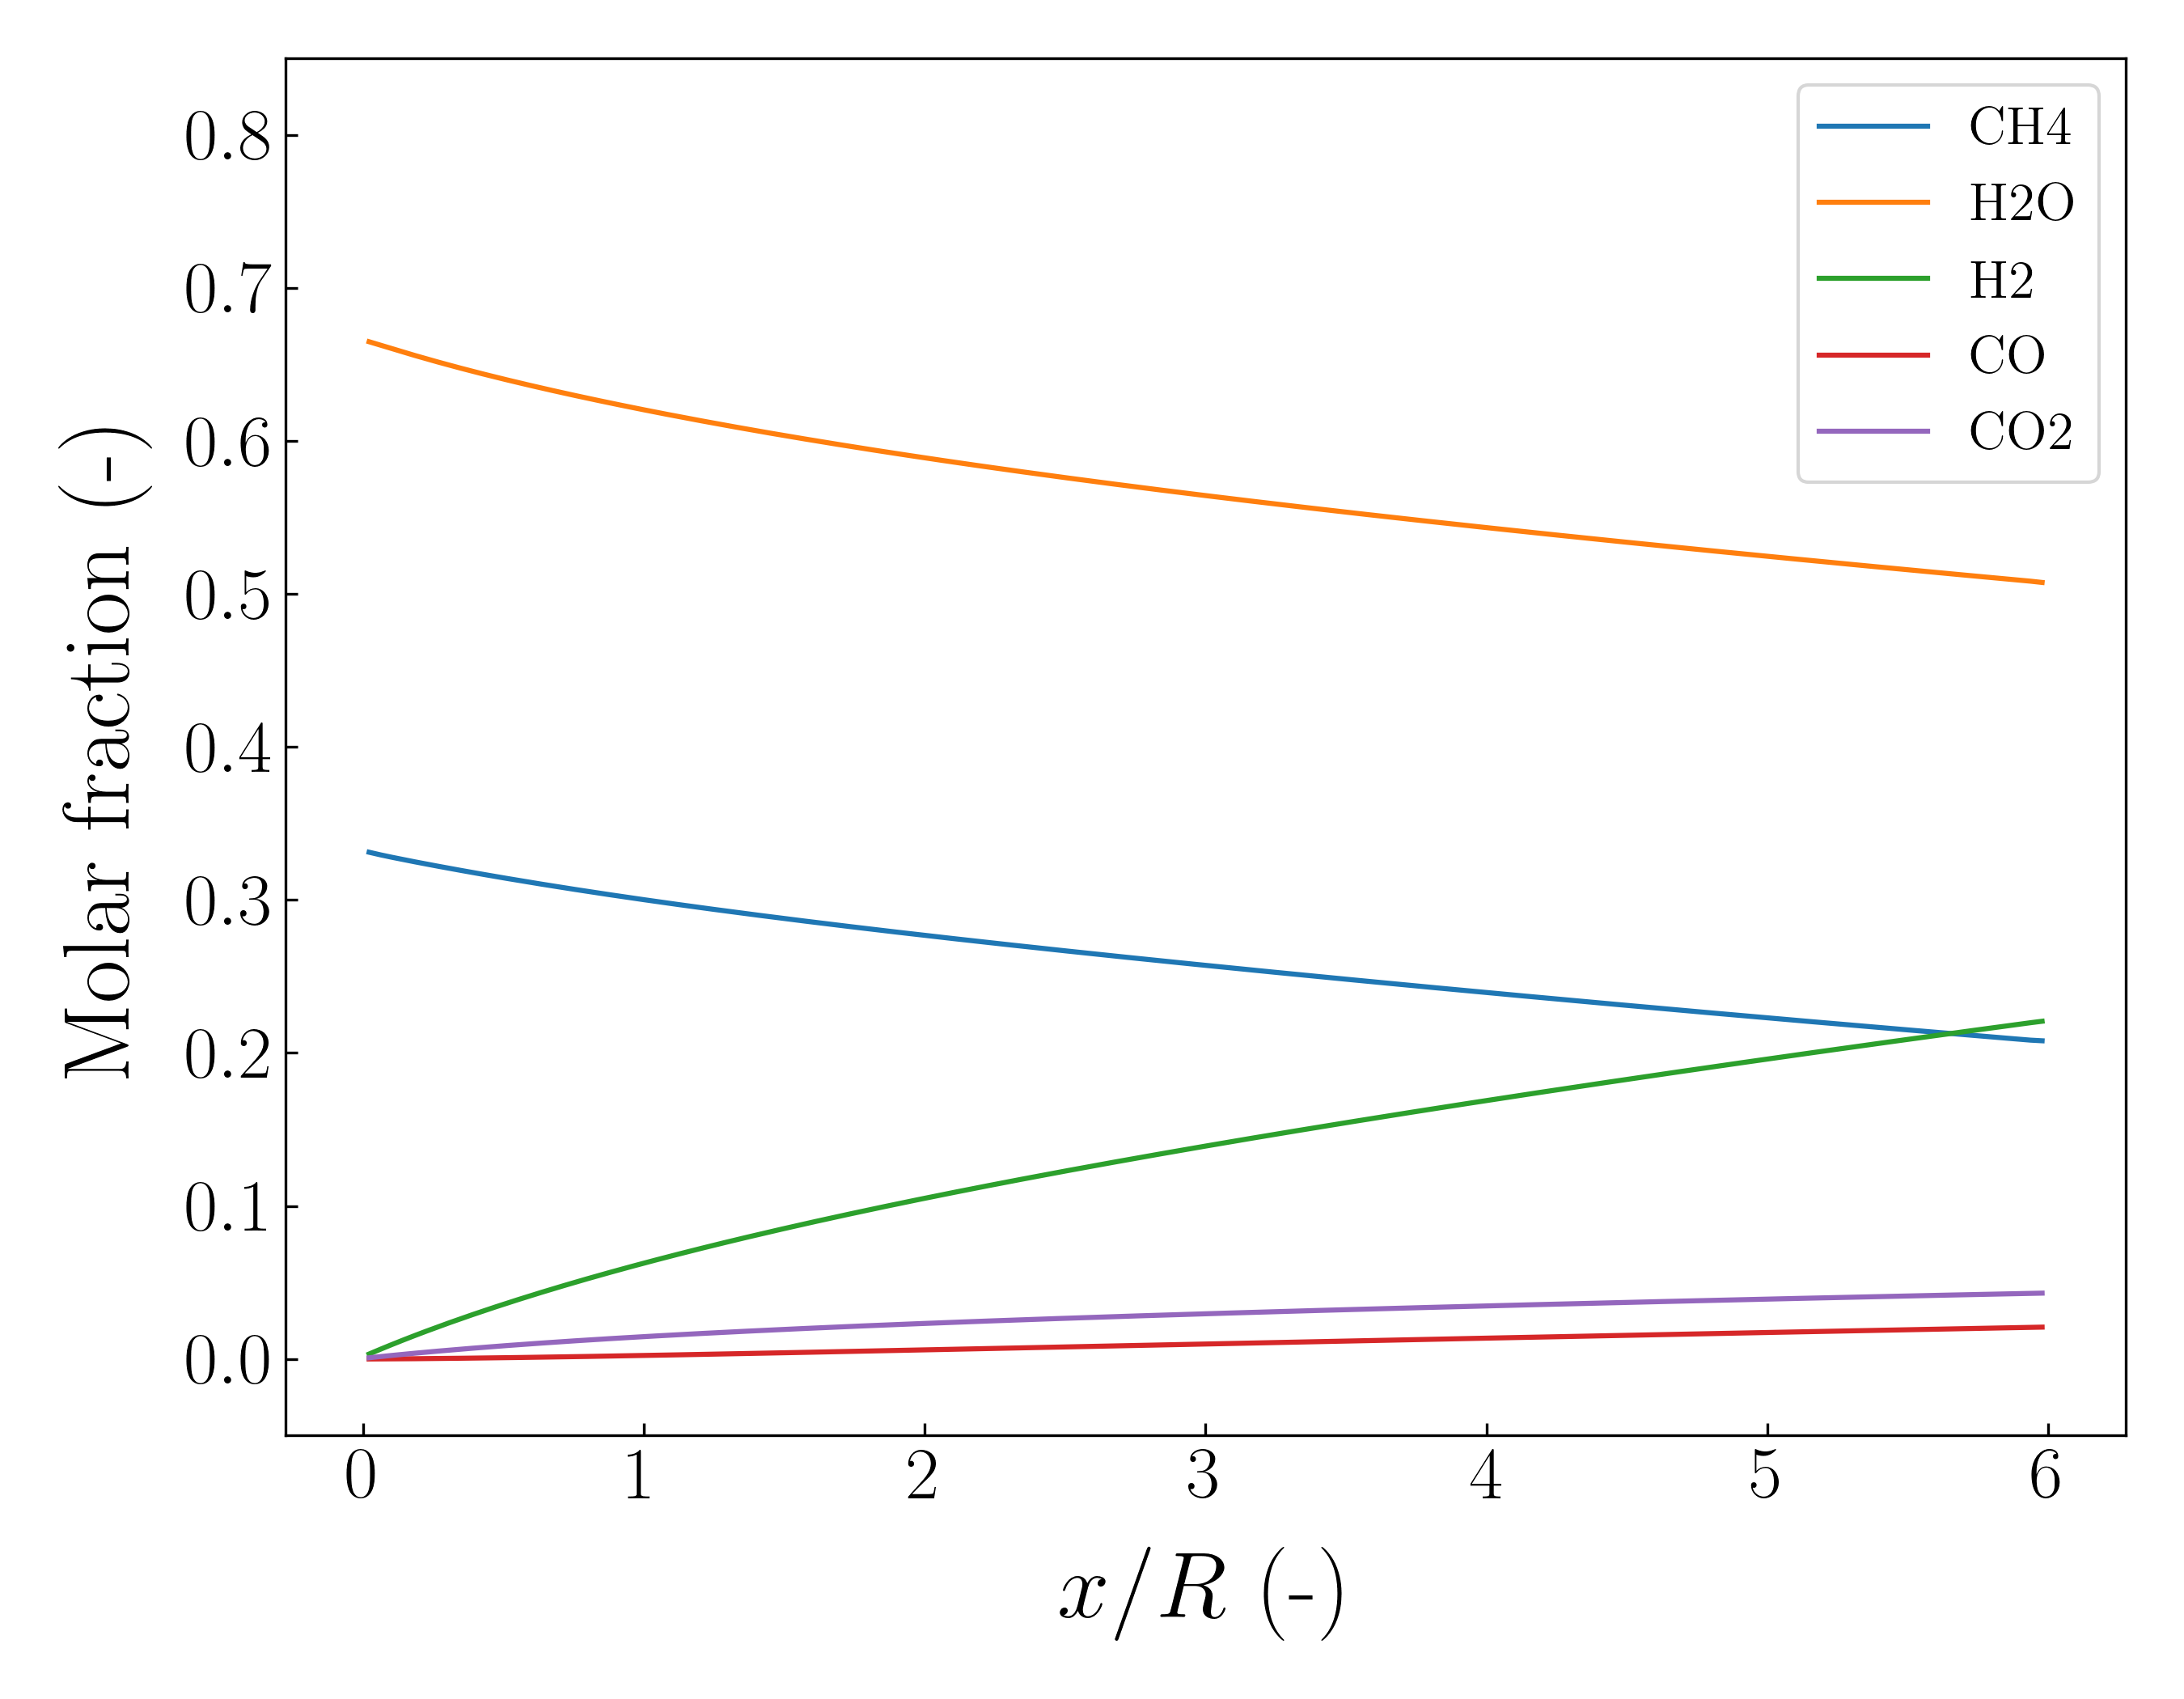
\includegraphics[width=80mm]{results/5/40C_60T/GEN15-AVG.png}
%\caption{\label{fig:5R4060G15-avg} Strategy I - Radius-averaged molar fractions - 15$^{\rm{th}}$ generation ($w_{\rm{CH_4}} = 0.4, w_T = 0.6$, $T_{\rm{in}}$ = 900 K, $u_{\rm{in}}$ = 0.15 m s$^{-1}$, $SC$ = 2.0)}
%\end{figure}
%
%\begin{figure}[h!]
%\centering
%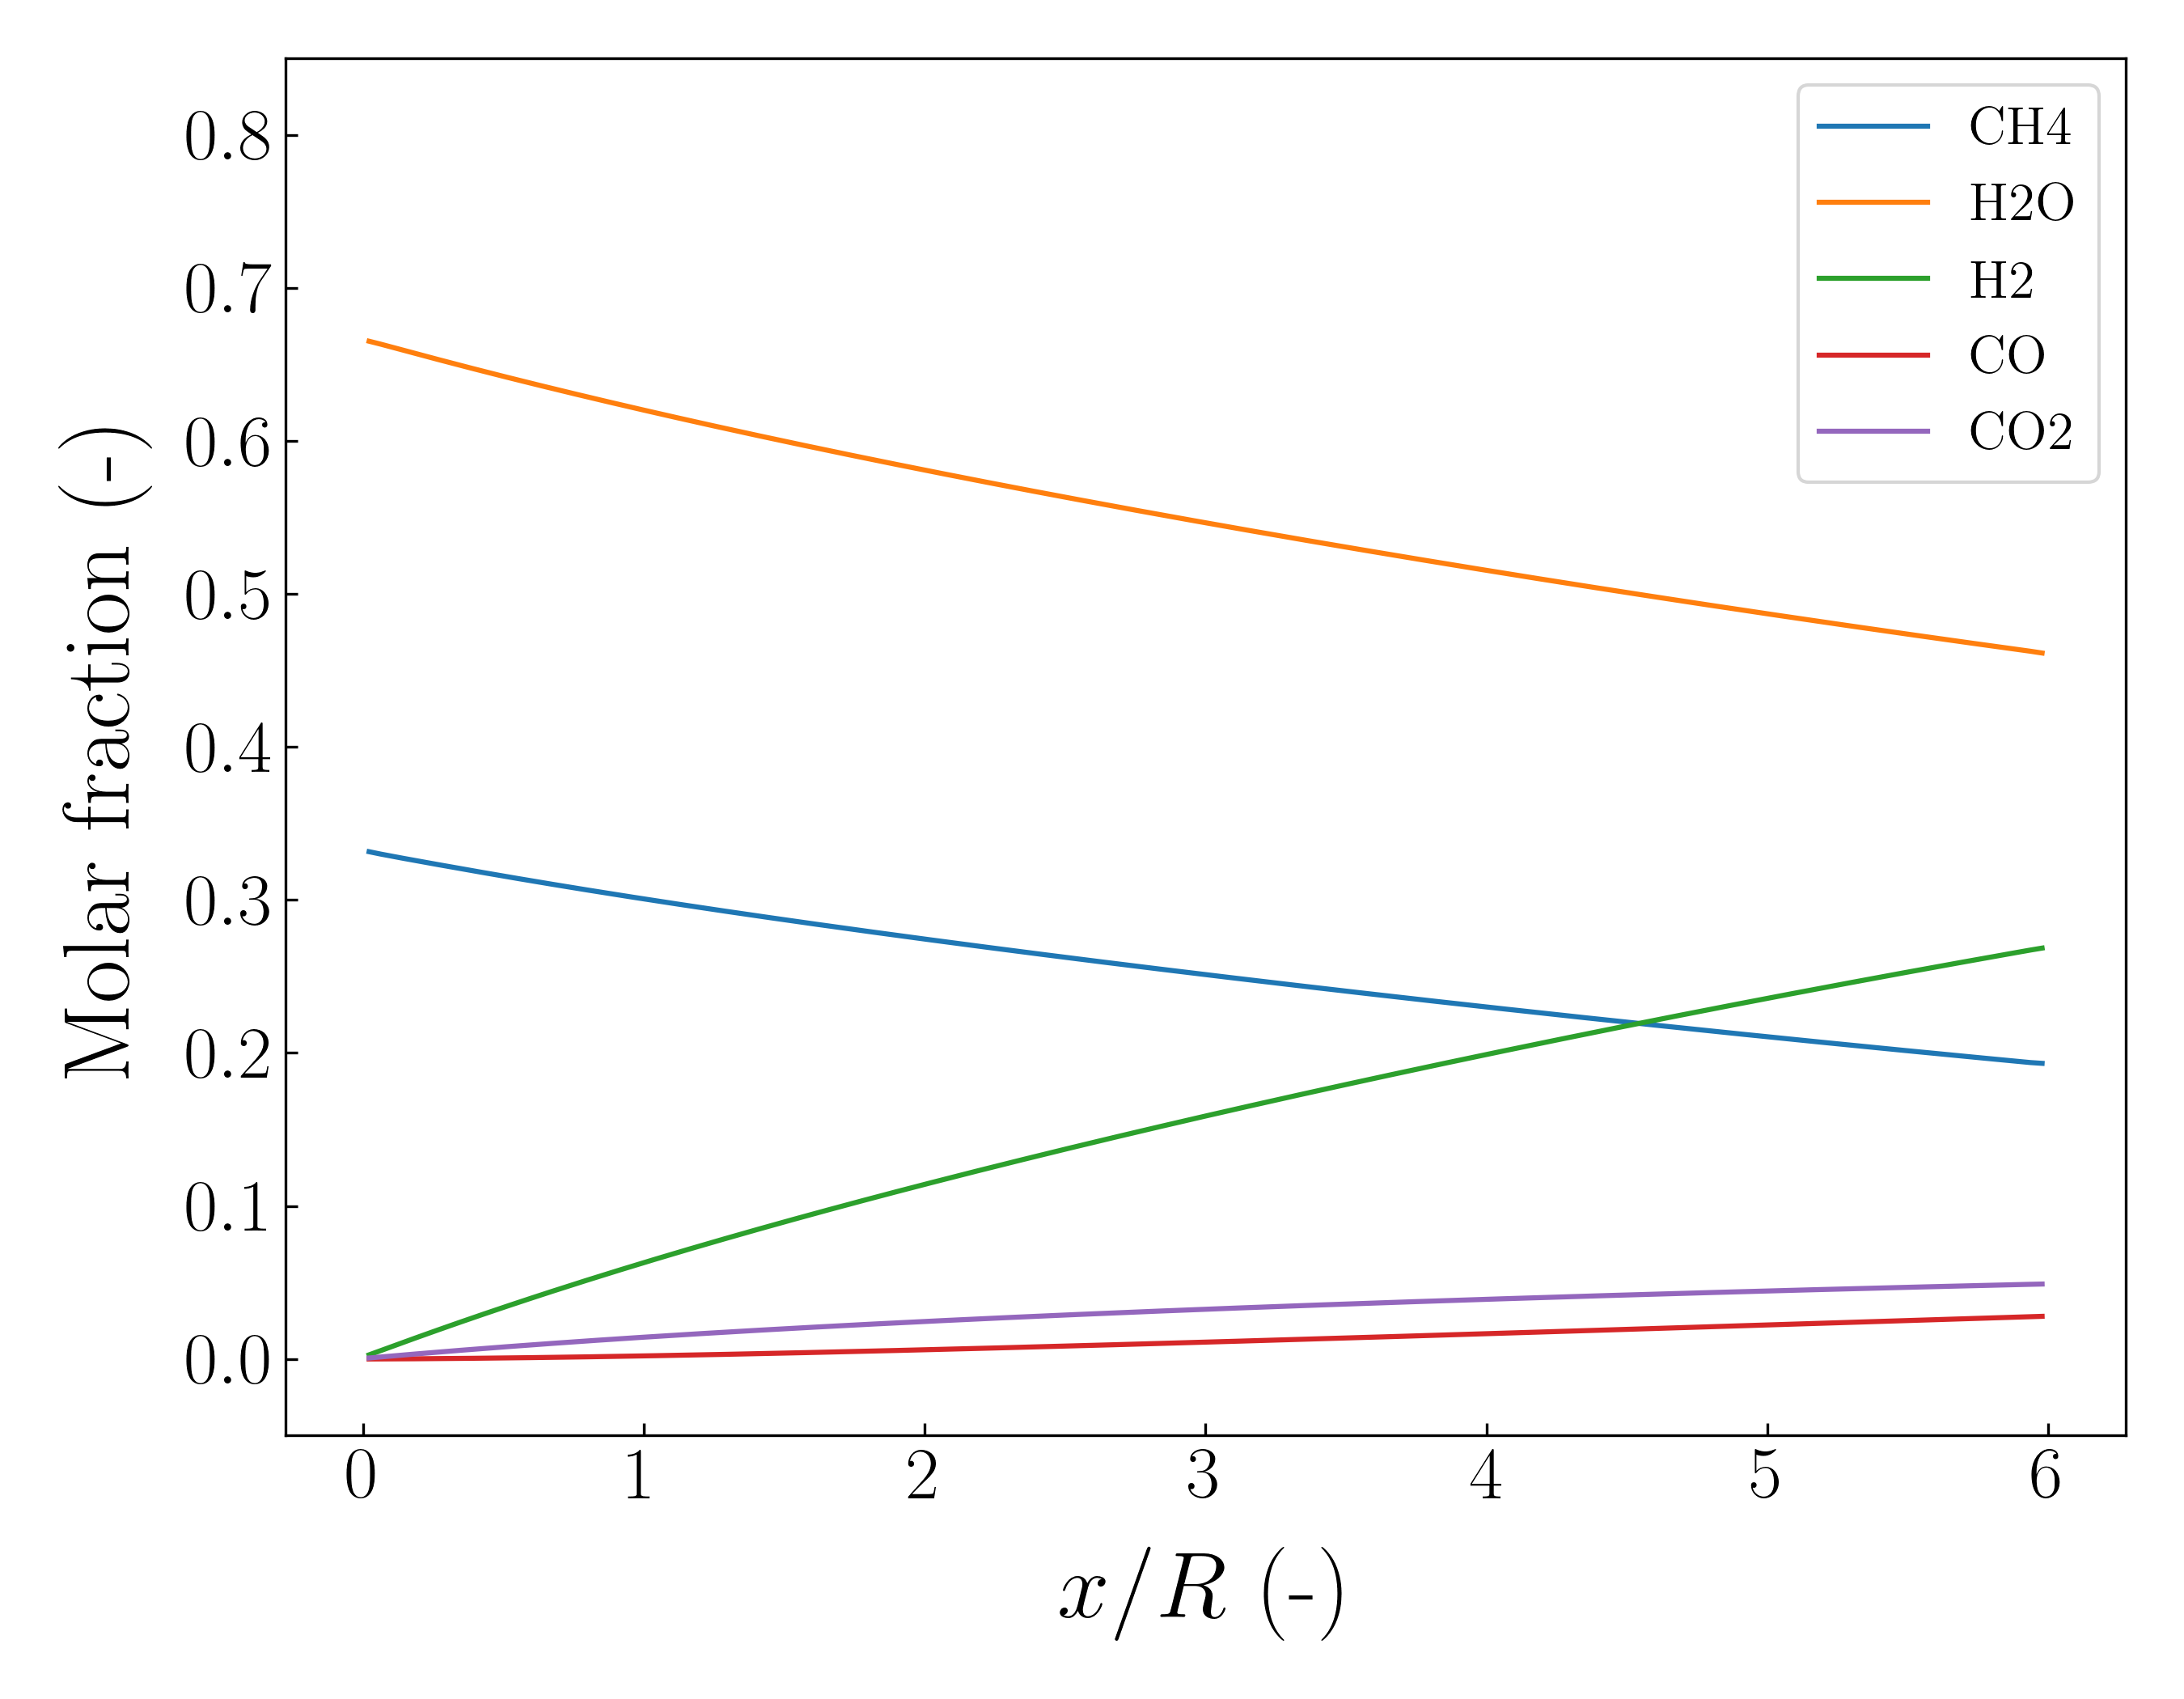
\includegraphics[width=80mm]{results/5/40C_60T/GEN30-AVG.png}
%\caption{\label{fig:5R4060G30-avg} Strategy I - Radius-averaged molar fractions -  30$^{\rm{th}}$ generation ($w_{\rm{CH_4}} = 0.4, w_T = 0.6$, $T_{\rm{in}}$ = 900 K, $u_{\rm{in}}$ = 0.15 m s$^{-1}$, $SC$ = 2.0)}
%\end{figure}
%
%\begin{figure}[h!]
%\centering
%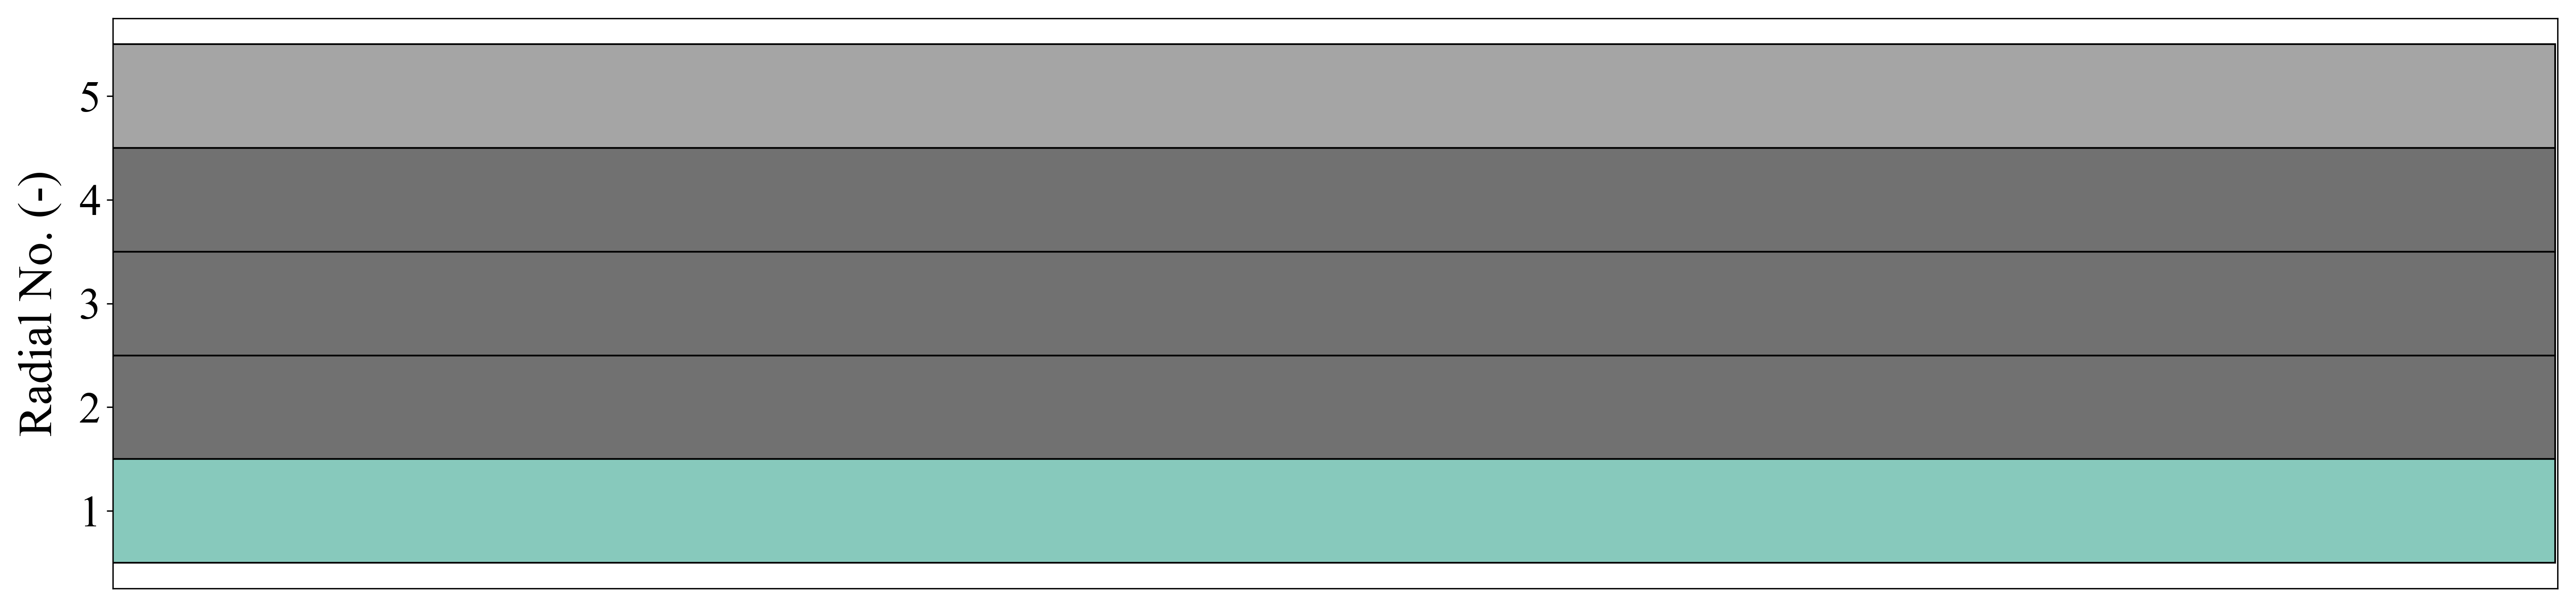
\includegraphics[width=120mm]{results/segments/5seg/40C60T/seg.png}
%\caption{\label{fig:30L6040G1-TField} Strategy I - Segments distribution for 30$^{\rm{th}}$ generation ($w_{\rm{CH_4}} = 0.4, w_T = 0.6$, $T_{\rm{in}}$ = 900 K, $u_{\rm{in}}$ = 0.15 m s$^{-1}$, $SC$ = 2.0)}
%\end{figure}
%
%\begin{figure}[h!]
%\centering
%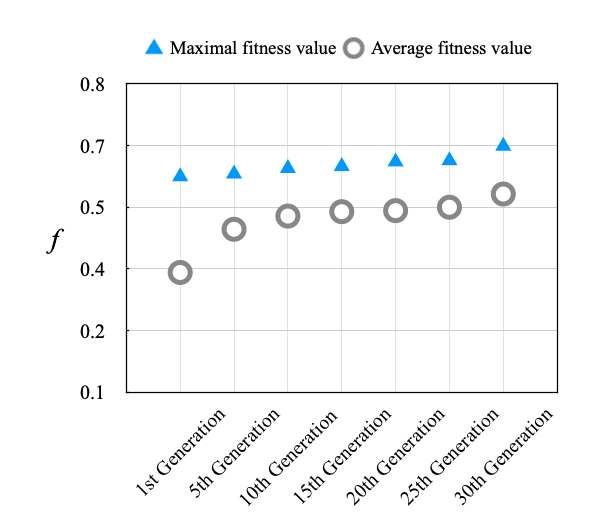
\includegraphics[width=100mm]{results/5/40C_60T.png}
%\caption{\label{fig:5R4060G-fitness} Strategy I - Fitness analysis throughout successive populations ($w_{\rm{CH_4}} = 0.4, w_T = 0.6$, $T_{\rm{in}}$ = 900 K, $u_{\rm{in}}$ = 0.15 m s$^{-1}$, $SC$ = 2.0)}
%\end{figure}
%
%
%\clearpage
%
%
%
%
%
%\paragraph{Thermal fitness 50 \%, methane conversion 50 \%} \hspace{0pt} \\
%\noindent 
%
%
%\begin{figure}[h!]
%\centering
%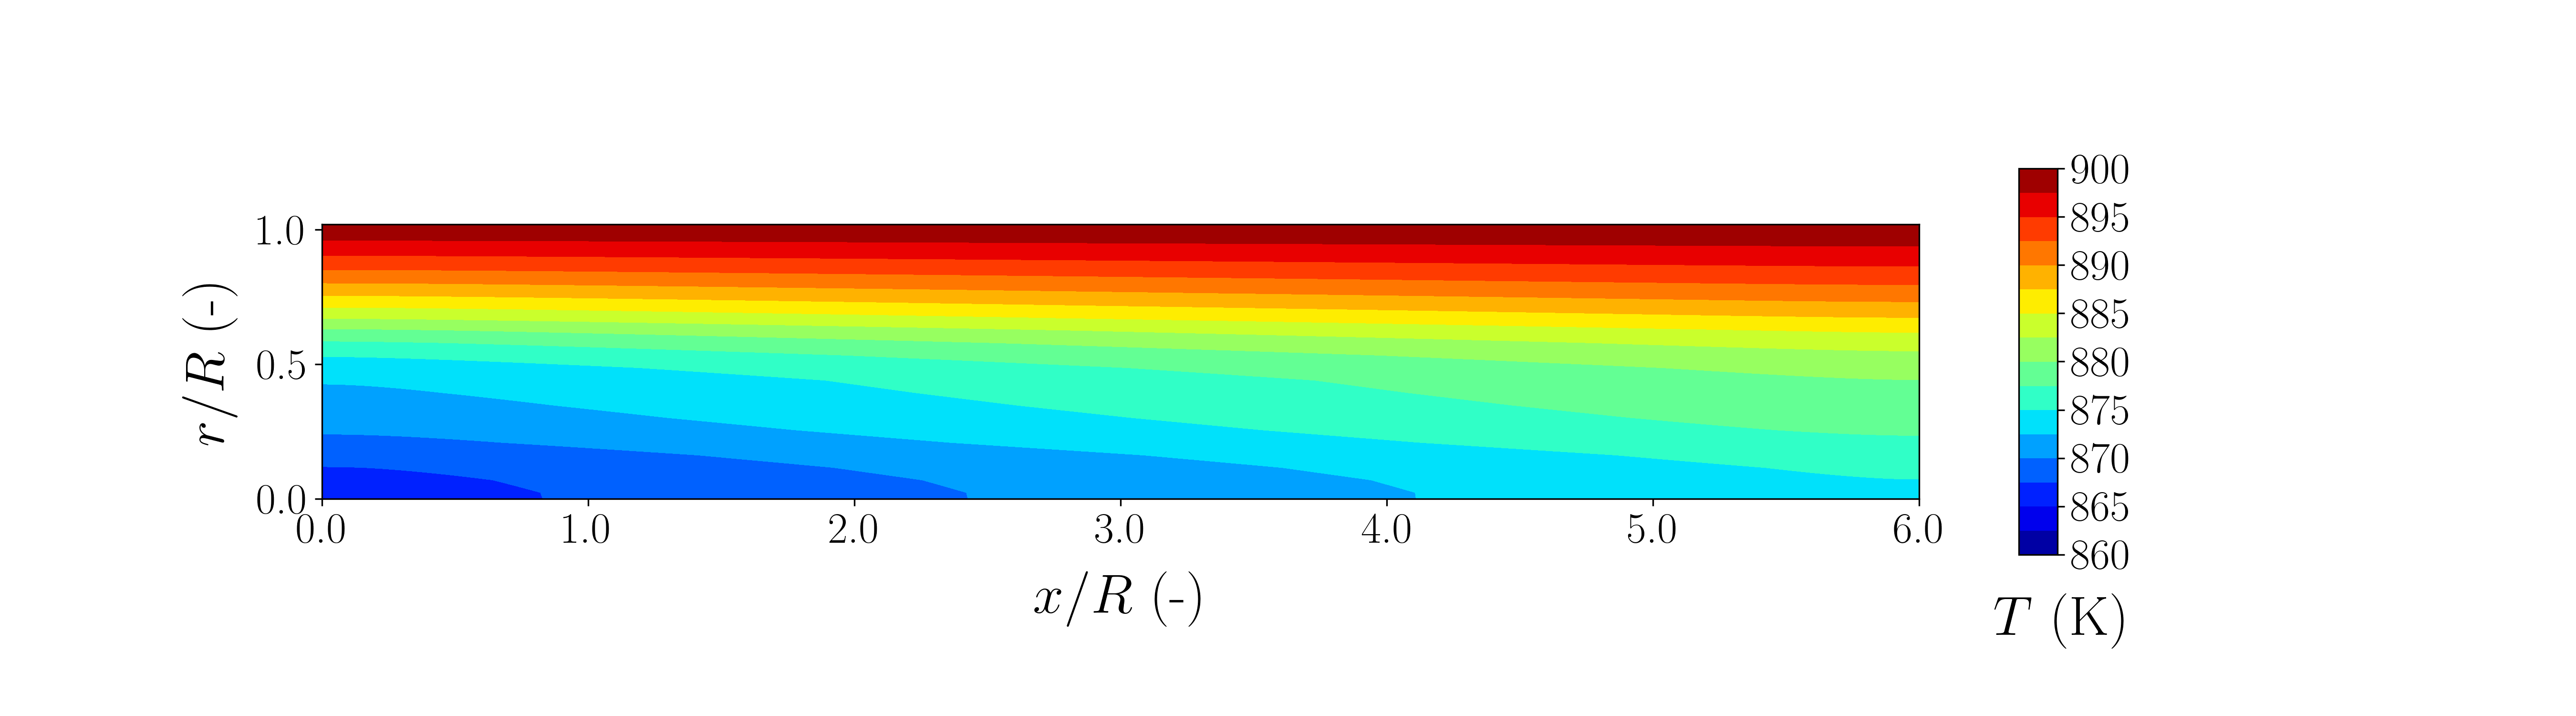
\includegraphics[width=190mm]{results/5/50C_50T/GEN1-TFIELD.png}
%\caption{\label{fig:5R5050G1-TField} Strategy I - Temperature field distribution - 1$^{\rm{st}}$ generation ($w_{\rm{CH_4}} = 0.5, w_T = 0.5$, $T_{\rm{in}}$ = 900 K, $u_{\rm{in}}$ = 0.15 m s$^{-1}$, $SC$ = 2.0)}
%\end{figure}
%
%\begin{figure}[h!]
%\centering
%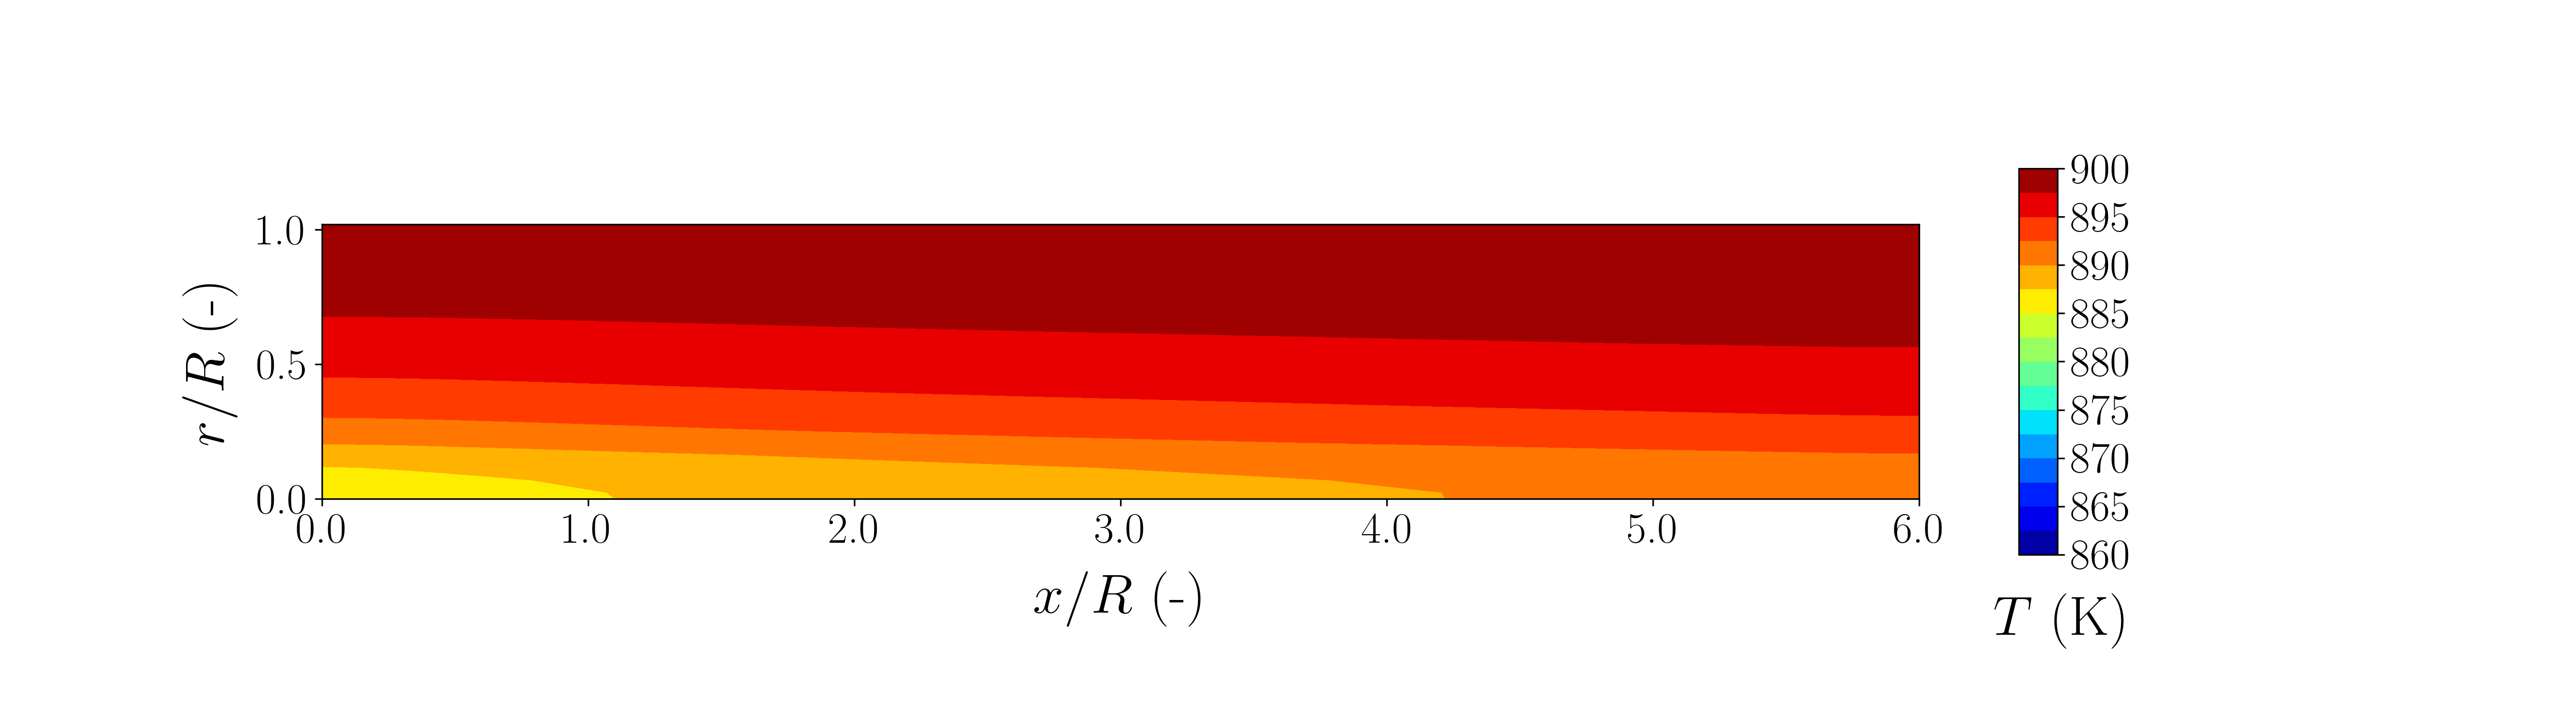
\includegraphics[width=190mm]{results/5/50C_50T/GEN15-TFIELD.png}
%\caption{\label{fig:5R5050G15-TField} Strategy I - Temperature field distribution - 15$^{\rm{th}}$ generation ($w_{\rm{CH_4}} = 0.5, w_T = 0.5$, $T_{\rm{in}}$ = 900 K, $u_{\rm{in}}$ = 0.15 m s$^{-1}$, $SC$ = 2.0)}
%\end{figure}
%
%\begin{figure}[h!]
%\centering
%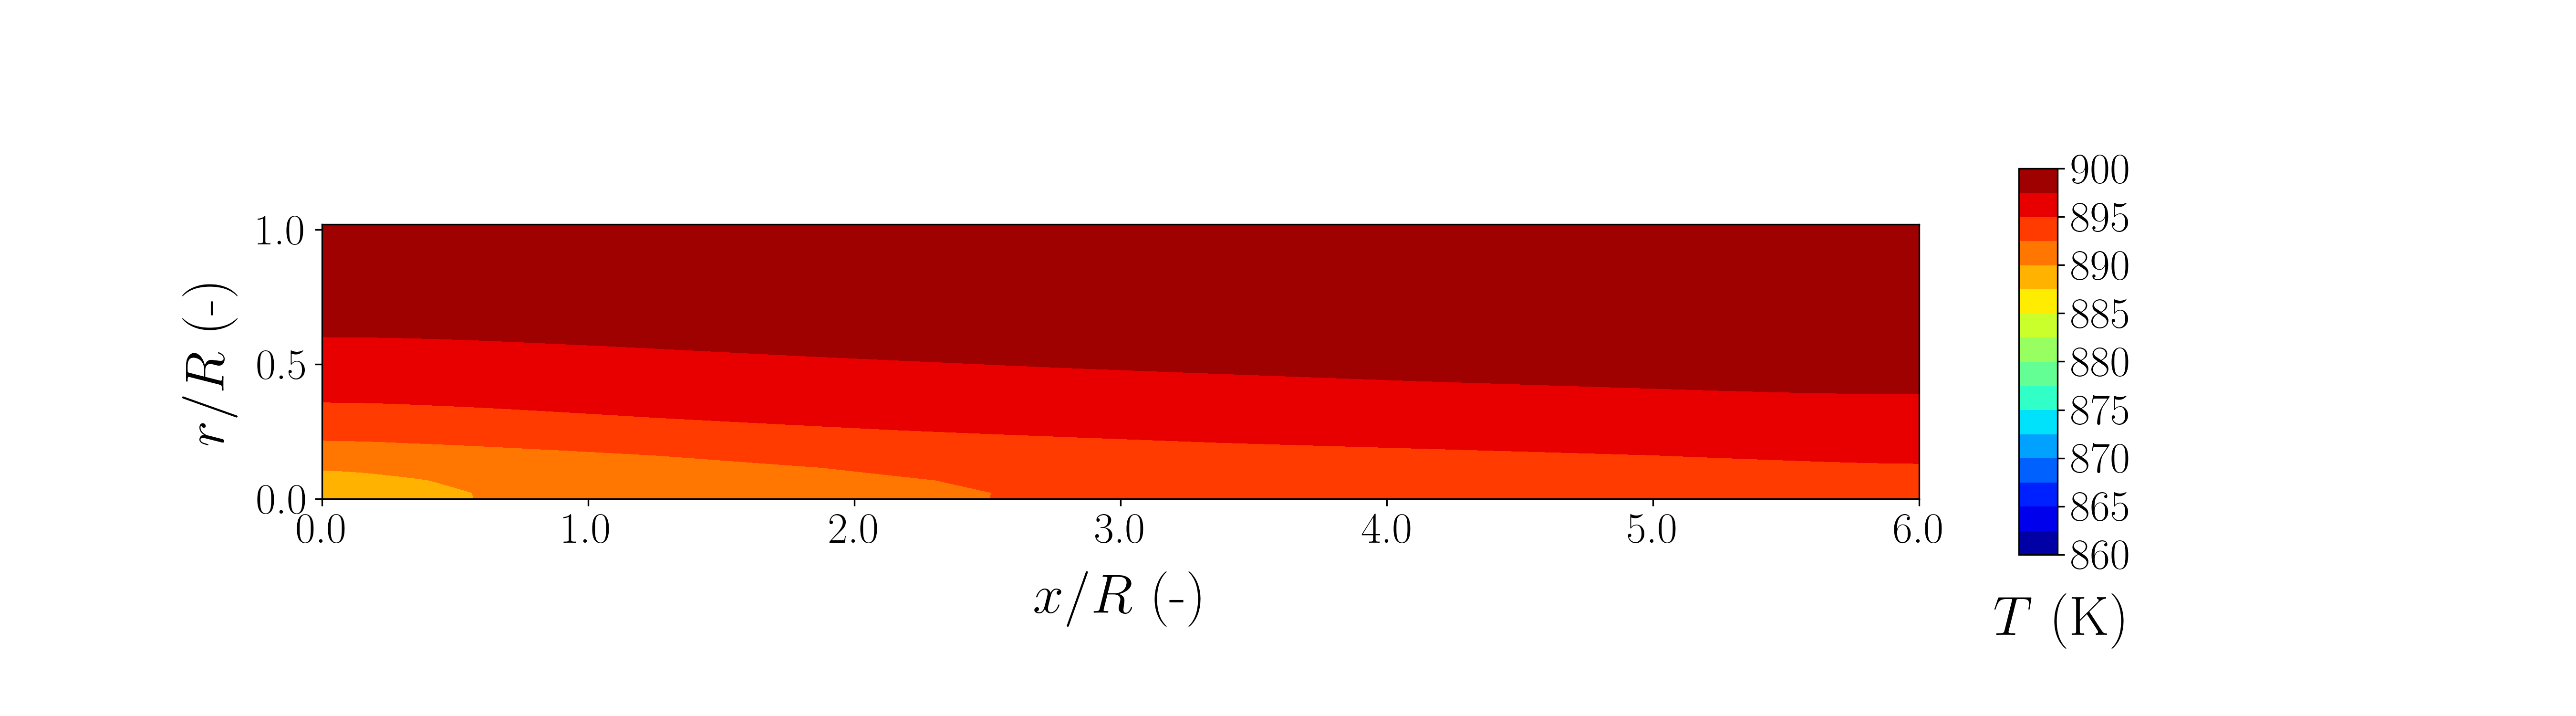
\includegraphics[width=190mm]{results/5/50C_50T/GEN30-TFIELD.png}
%\caption{\label{fig:5R5050G30-TField} Strategy I - Temperature field distribution - 30$^{\rm{th}}$ generation ($w_{\rm{CH_4}} = 0.5, w_T = 0.5$, $T_{\rm{in}}$ = 900 K, $u_{\rm{in}}$ = 0.15 m s$^{-1}$, $SC$ = 2.0)}
%\end{figure}
%
%
%\begin{figure}[h!]
%\centering
%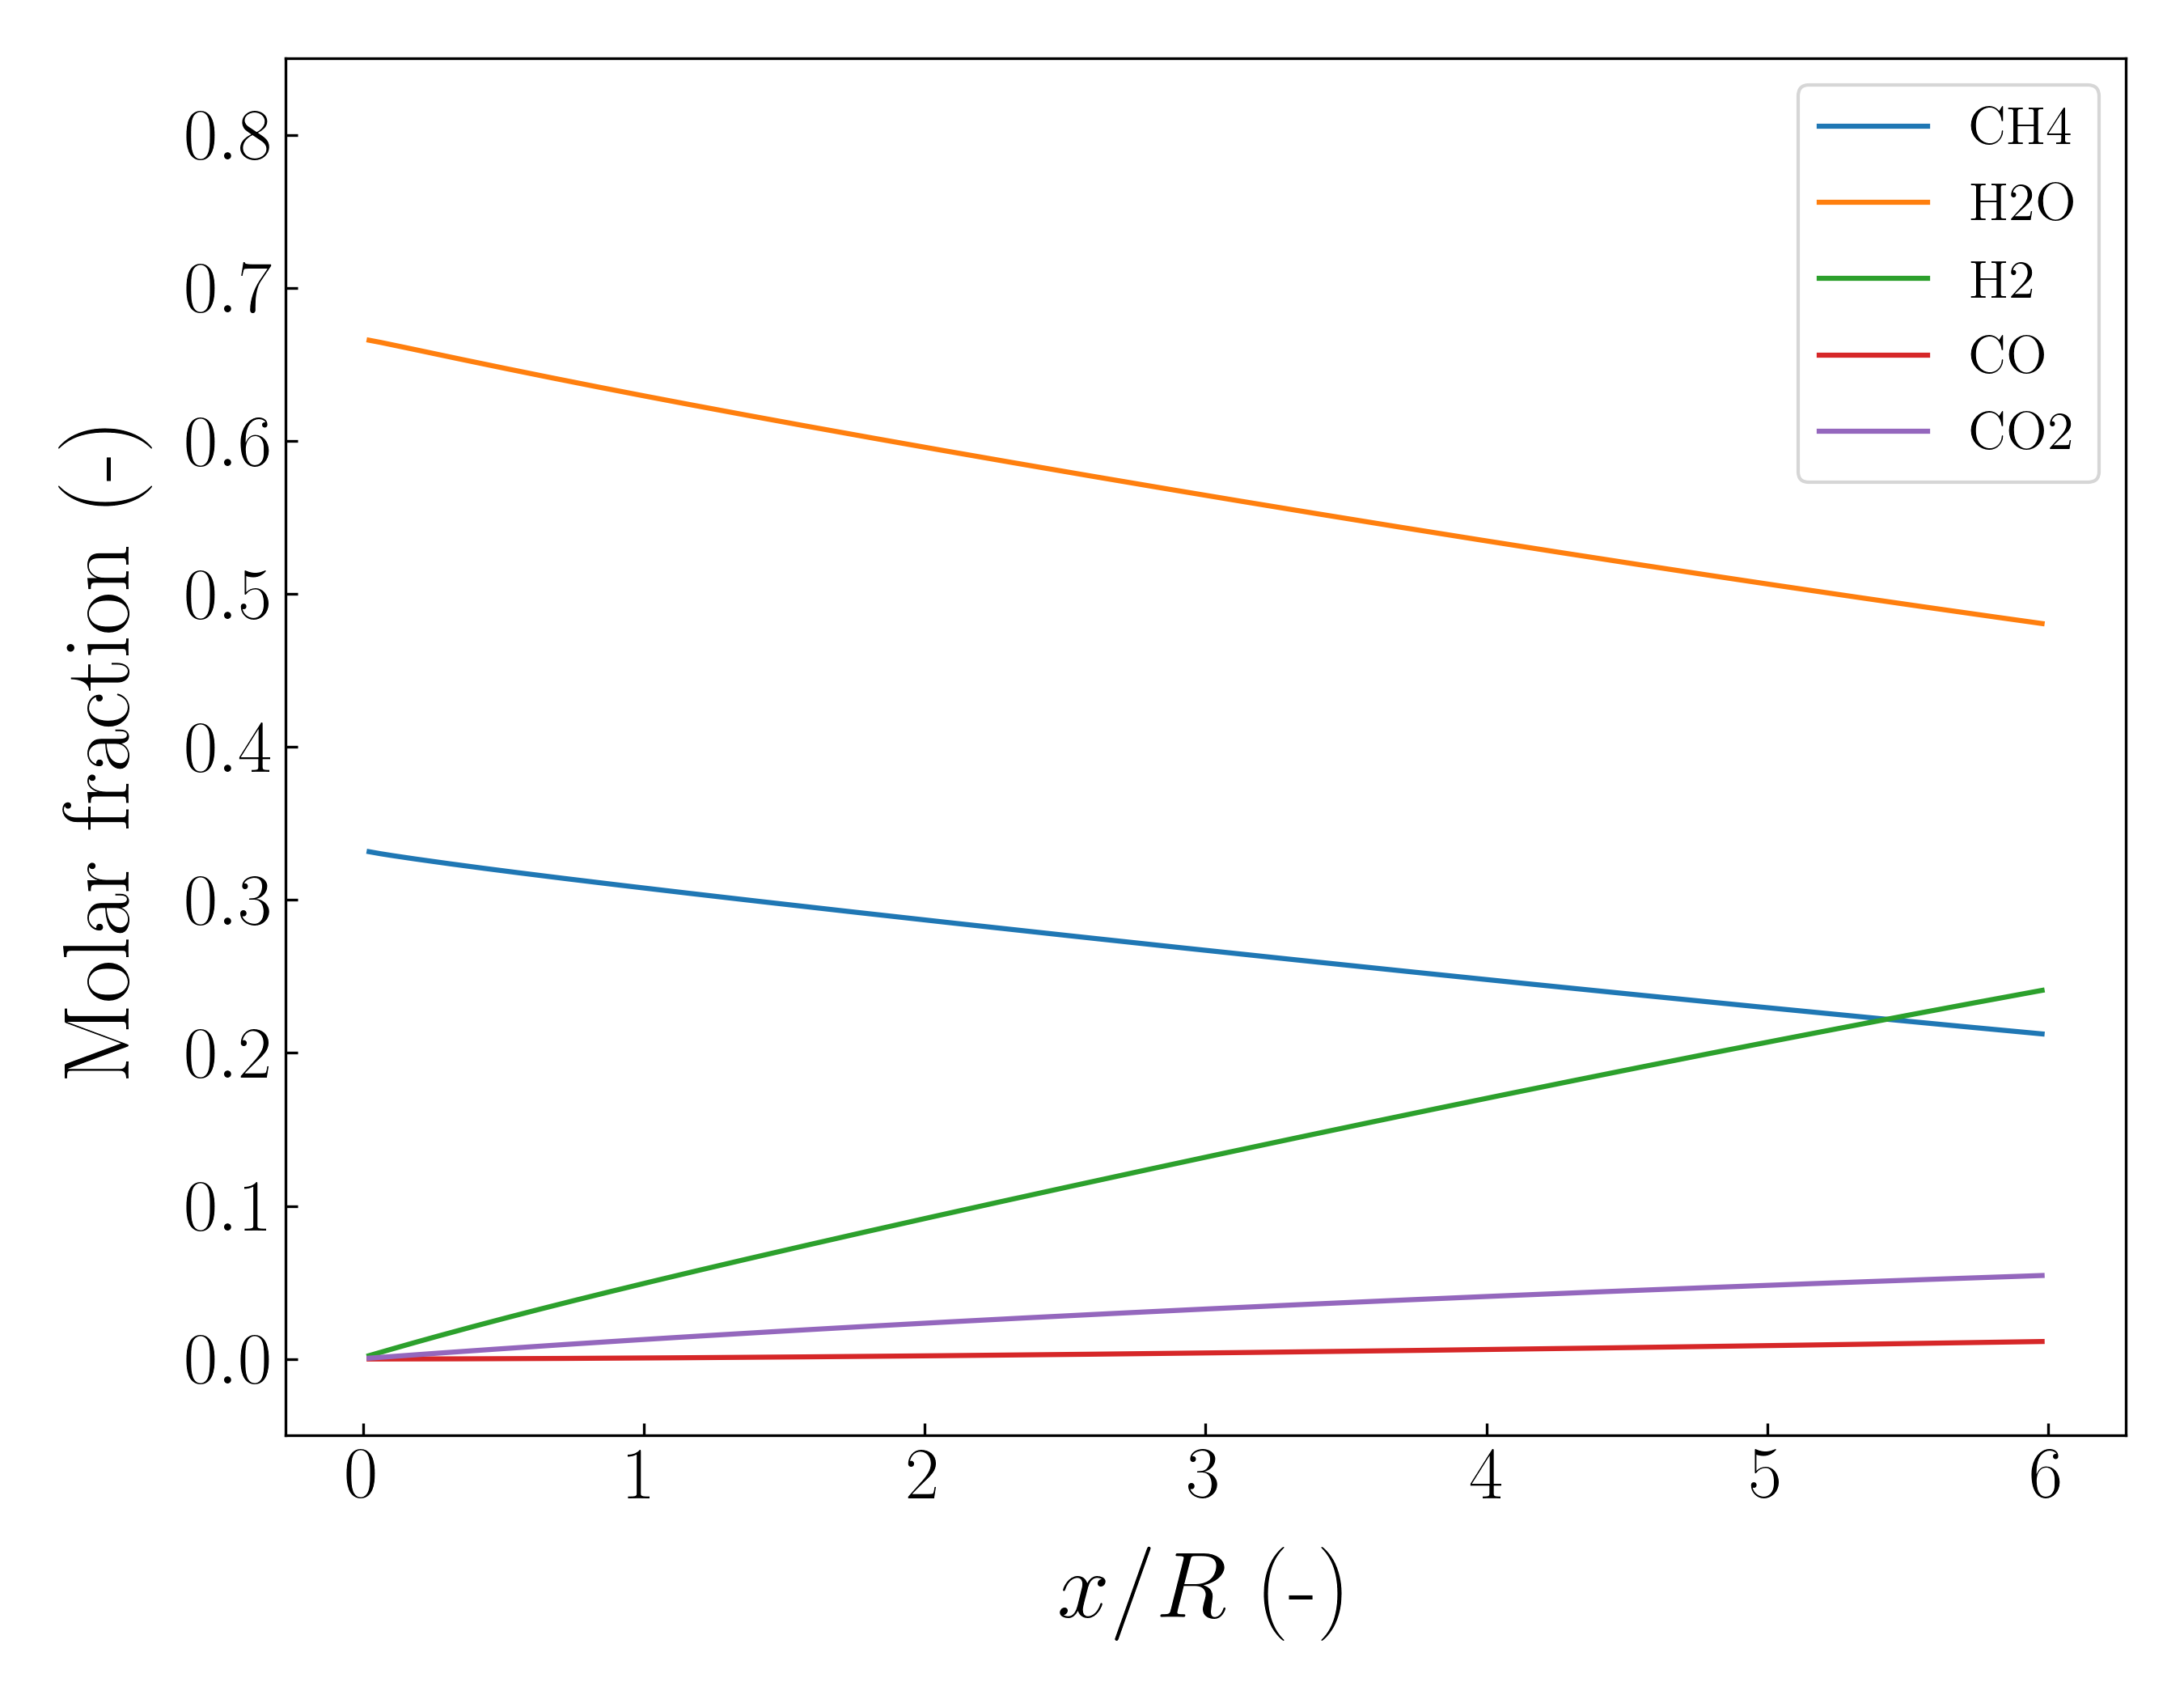
\includegraphics[width=80mm]{results/5/50C_50T/GEN1-AVG.png}
%\caption{\label{fig:5R5050G1-avg} Strategy I - Radius-averaged molar fractions - 1$^{\rm{st}}$ generation ($w_{\rm{CH_4}} = 0.5, w_T = 0.5$, $T_{\rm{in}}$ = 900 K, $u_{\rm{in}}$ = 0.15 m s$^{-1}$, $SC$ = 2.0)}
%\end{figure}
%
%\begin{figure}[h!]
%\centering
%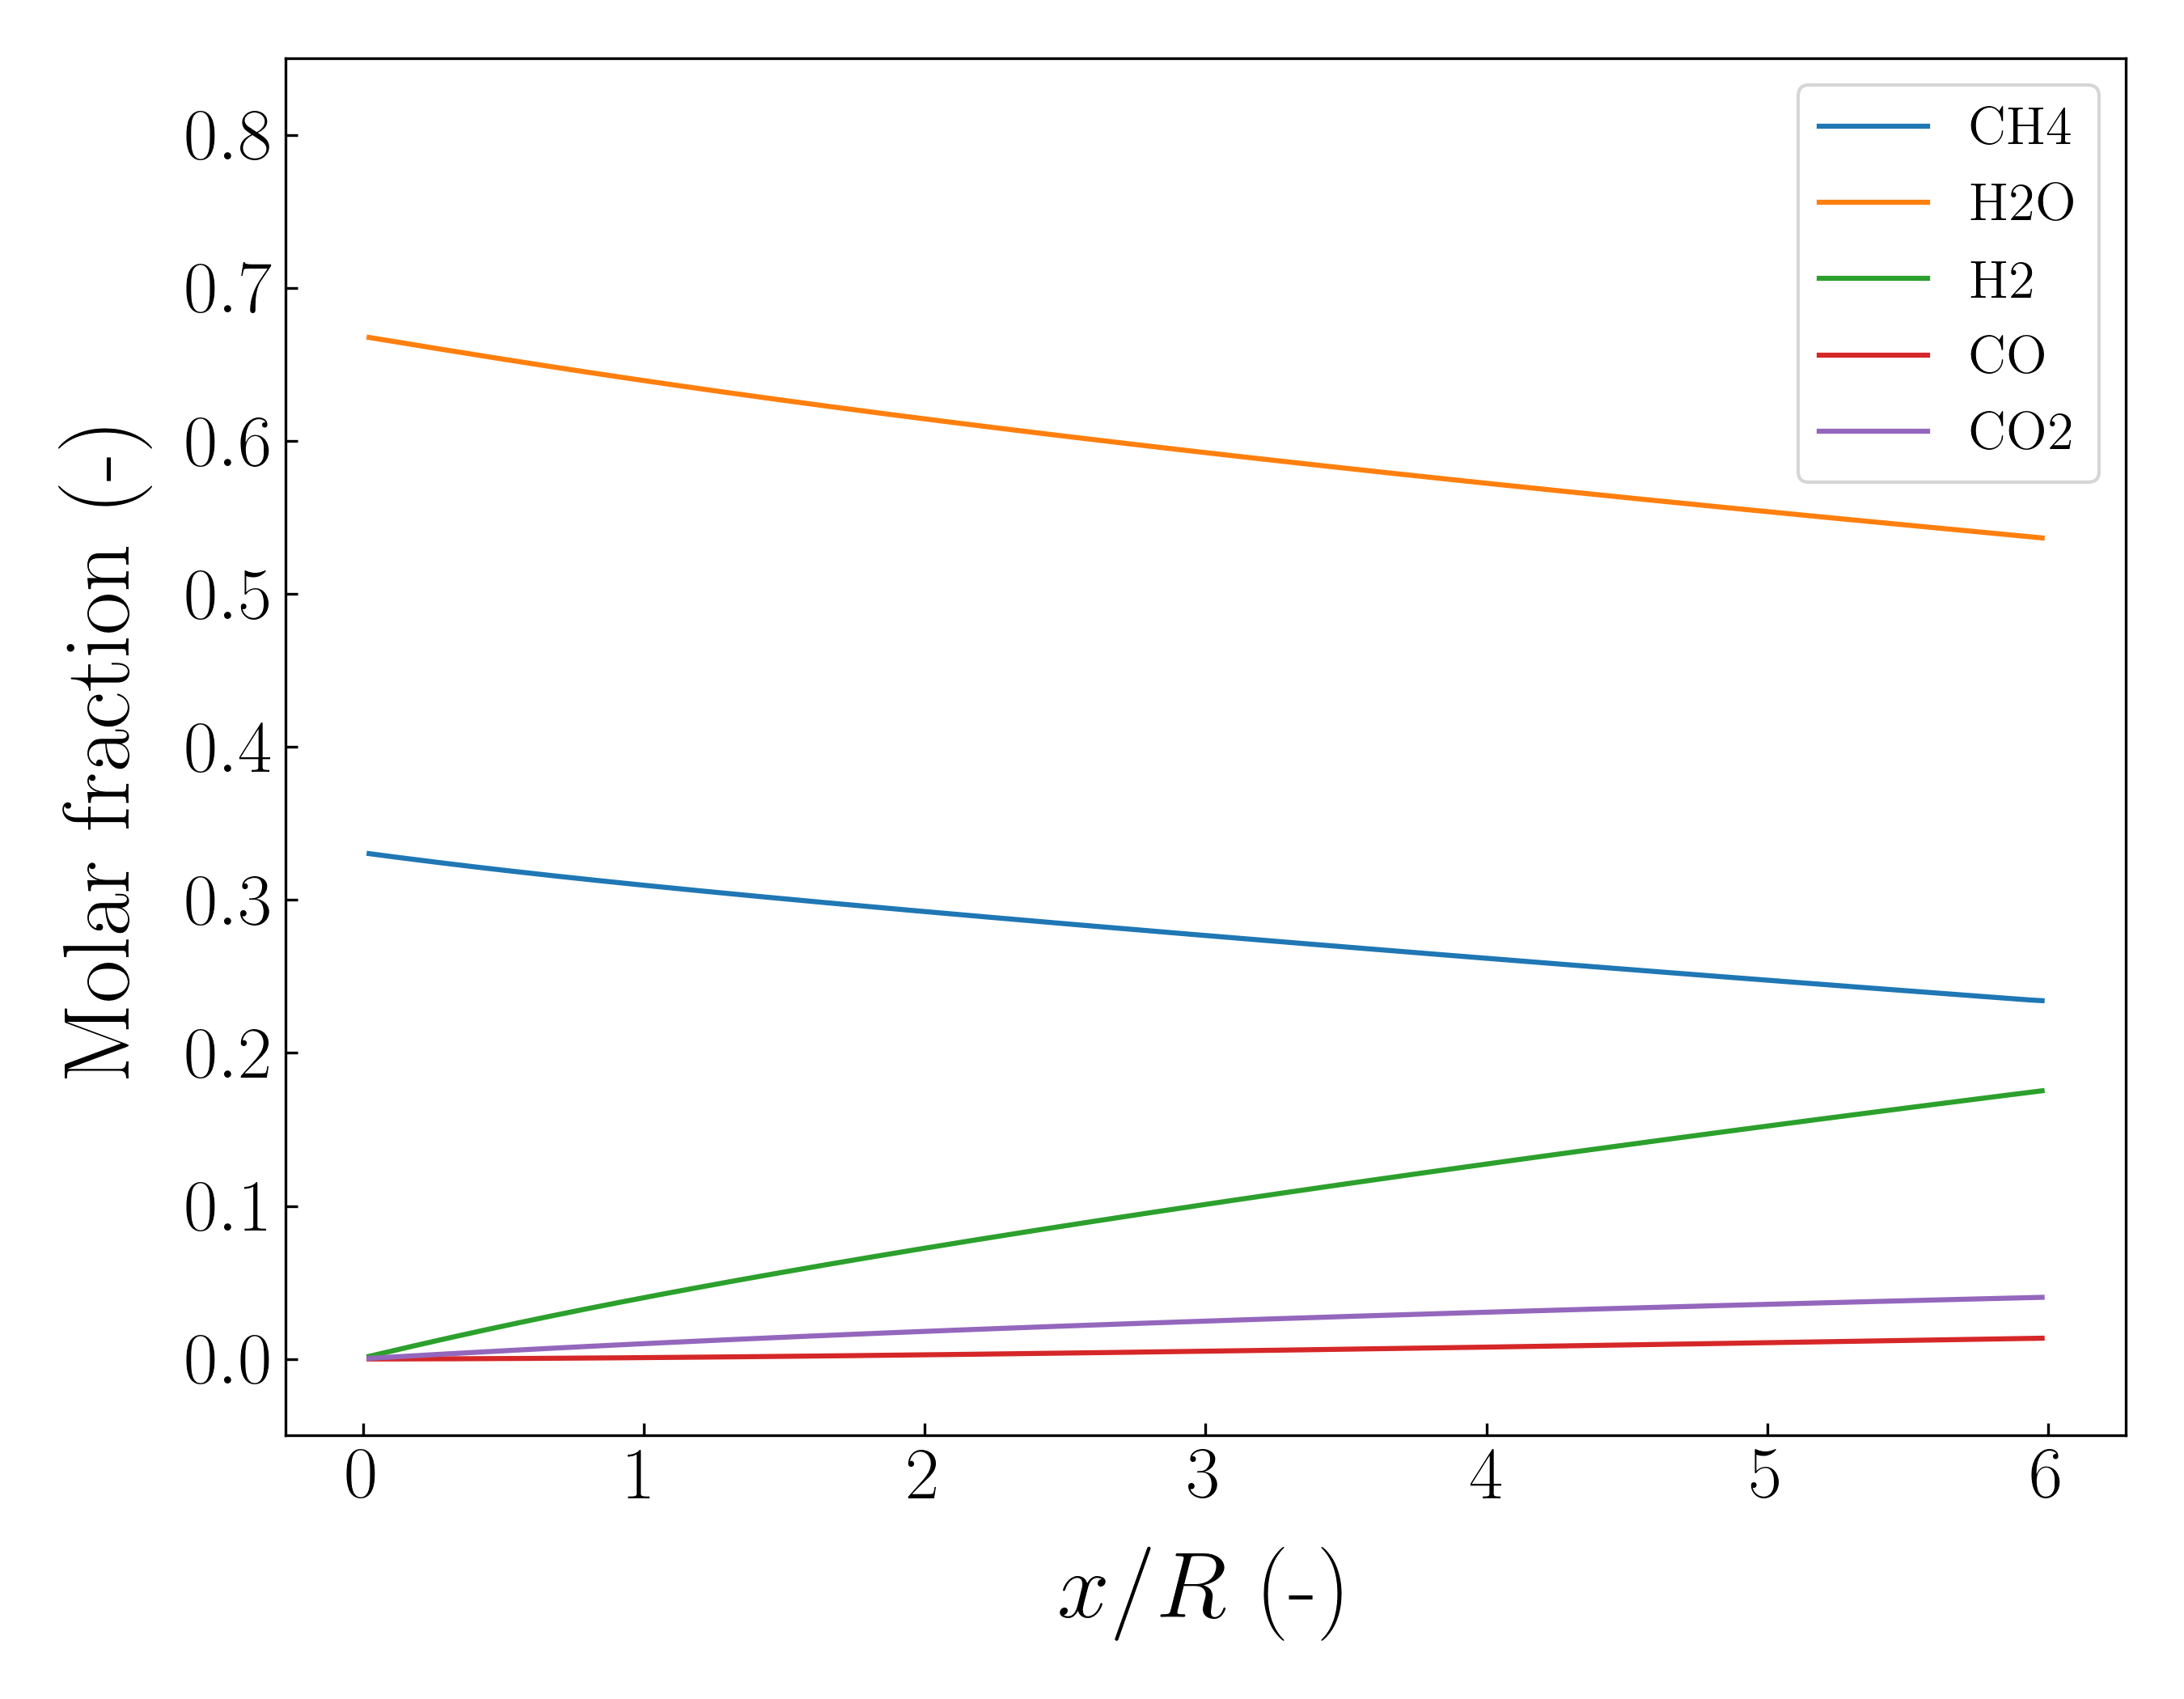
\includegraphics[width=80mm]{results/5/50C_50T/GEN15-AVG.png}
%\caption{\label{fig:5R5050G15-avg} Strategy I - Radius-averaged molar fractions - 15$^{\rm{th}}$ generation ($w_{\rm{CH_4}} = 0.5, w_T = 0.5$, $T_{\rm{in}}$ = 900 K, $u_{\rm{in}}$ = 0.15 m s$^{-1}$, $SC$ = 2.0)}
%\end{figure}
%
%\begin{figure}[h!]
%\centering
%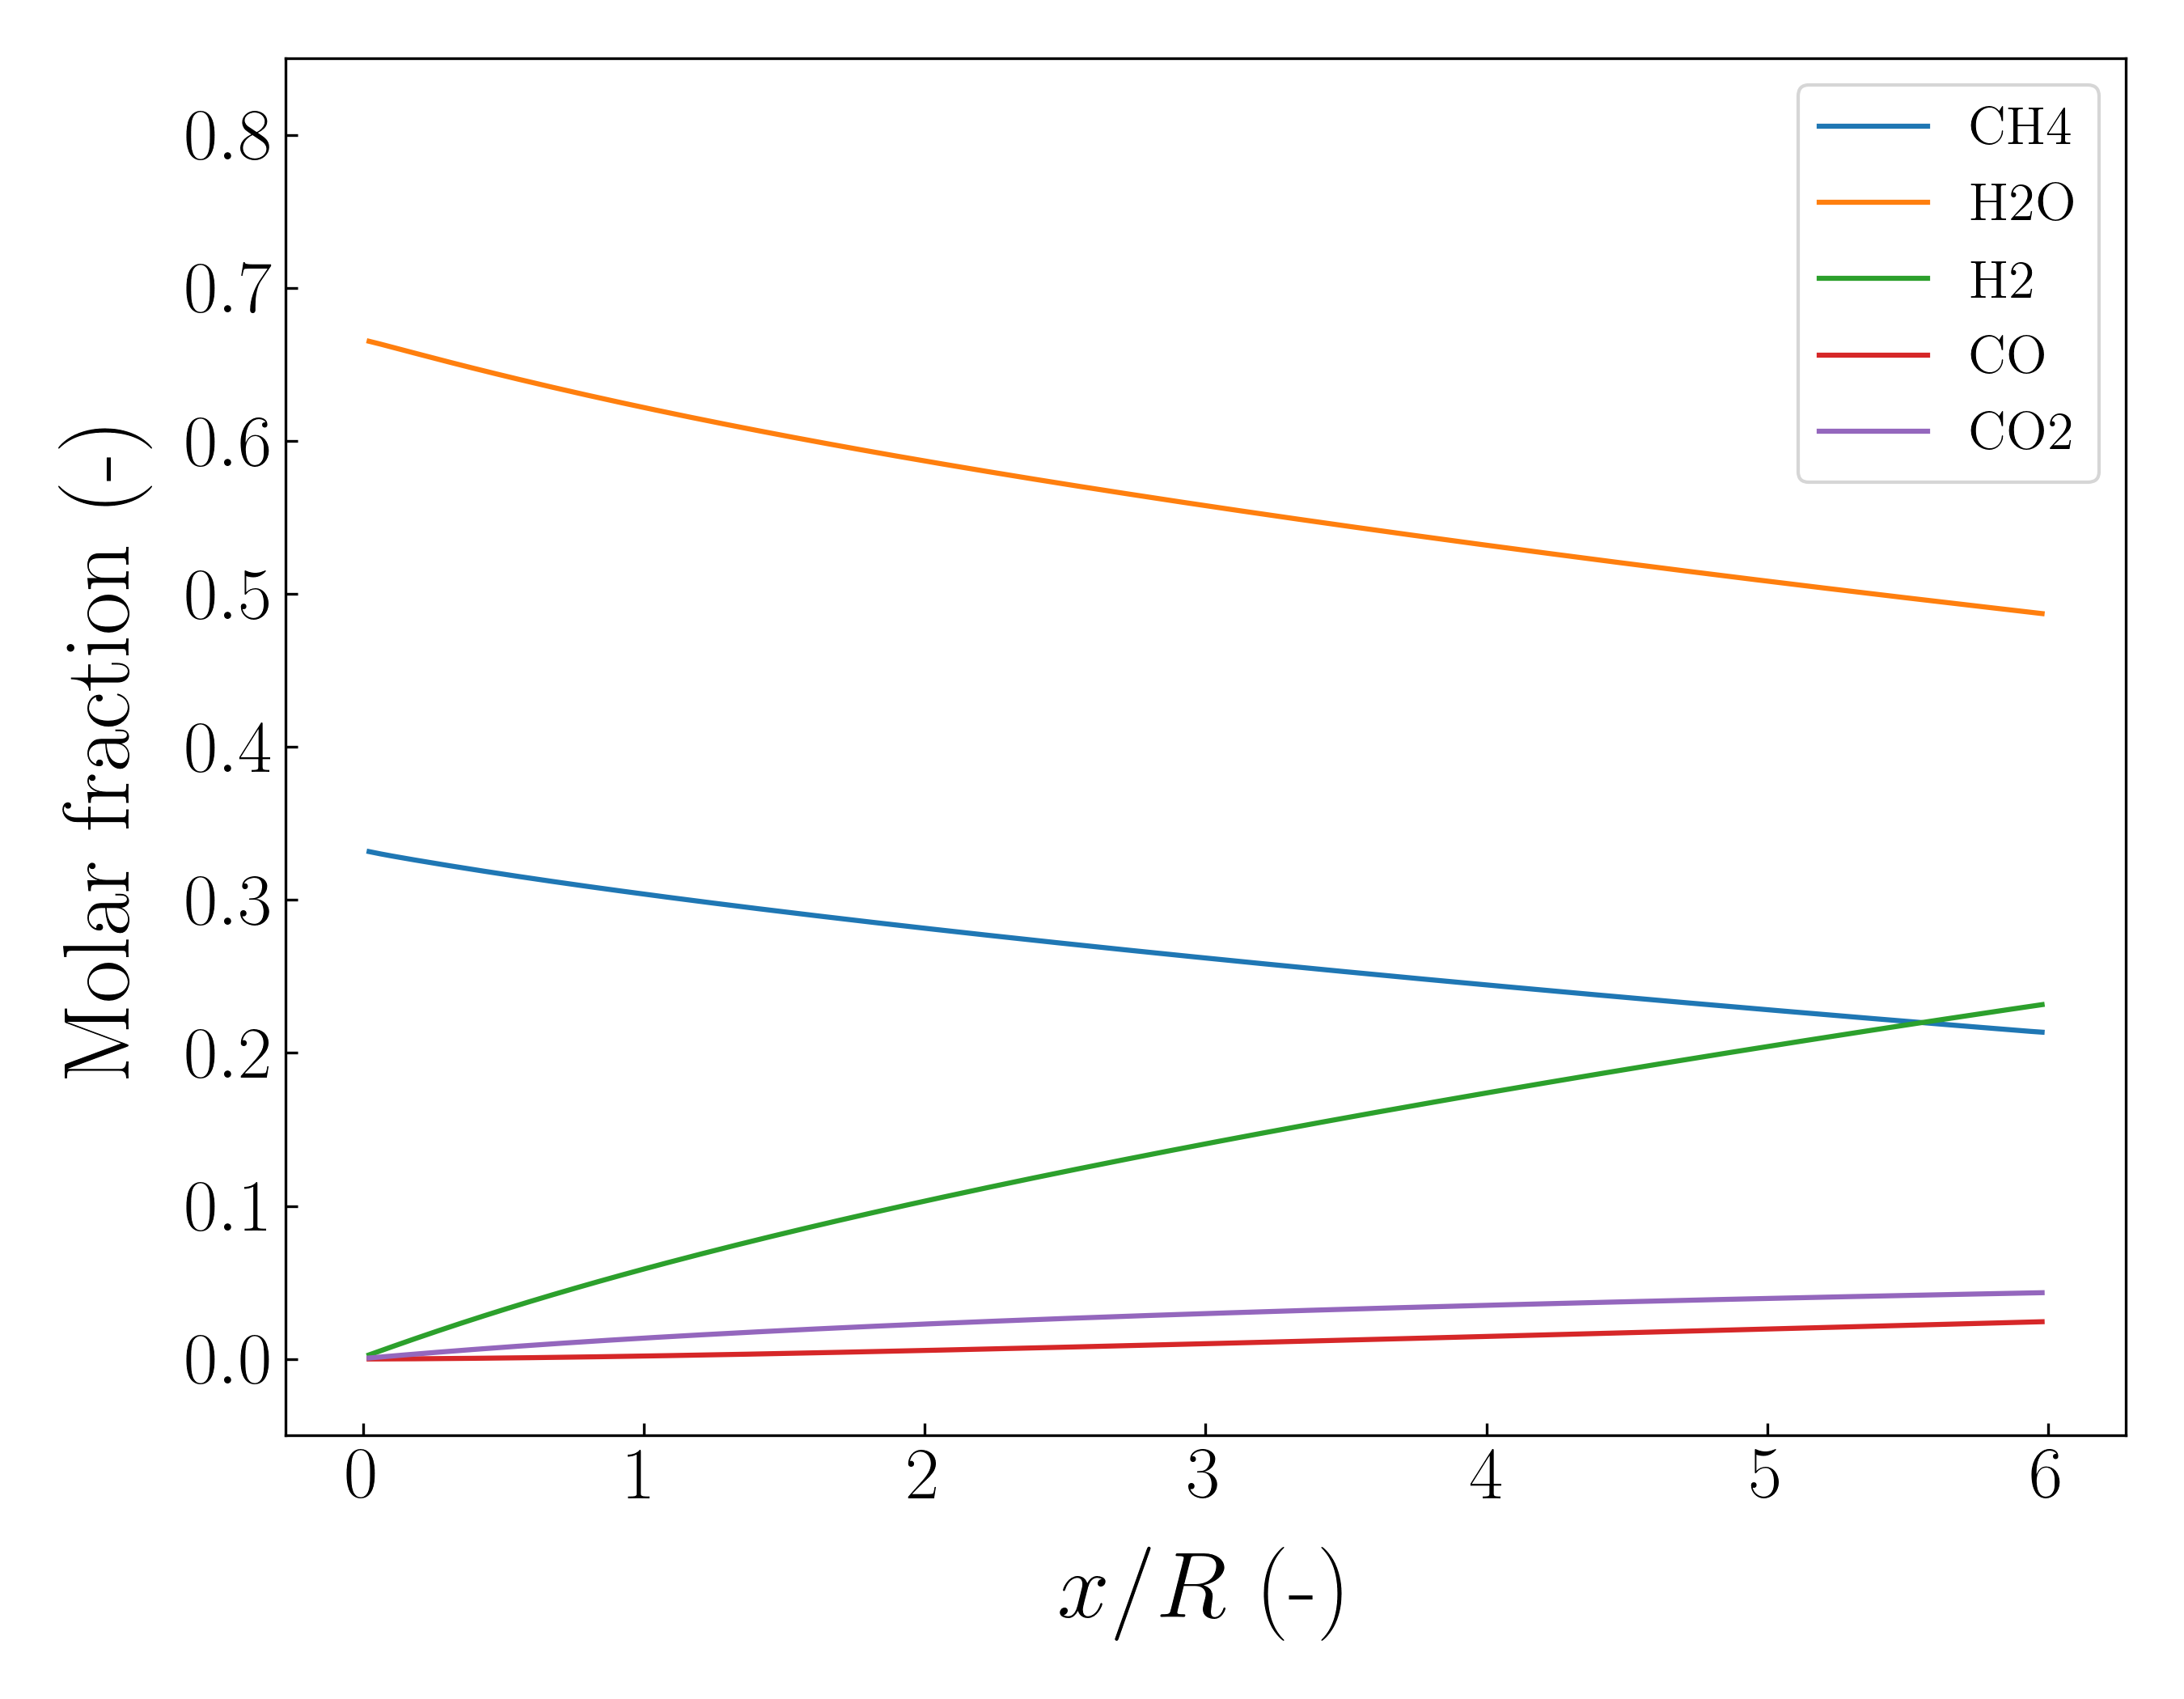
\includegraphics[width=80mm]{results/5/50C_50T/GEN30-AVG.png}
%\caption{\label{fig:5R5050G30-avg} Strategy I - Radius-averaged molar fractions -  30$^{\rm{th}}$ generation ($w_{\rm{CH_4}} = 0.5, w_T = 0.5$, $T_{\rm{in}}$ = 900 K, $u_{\rm{in}}$ = 0.15 m s$^{-1}$, $SC$ = 2.0)}
%\end{figure}
%
%\begin{figure}[h!]
%\centering
%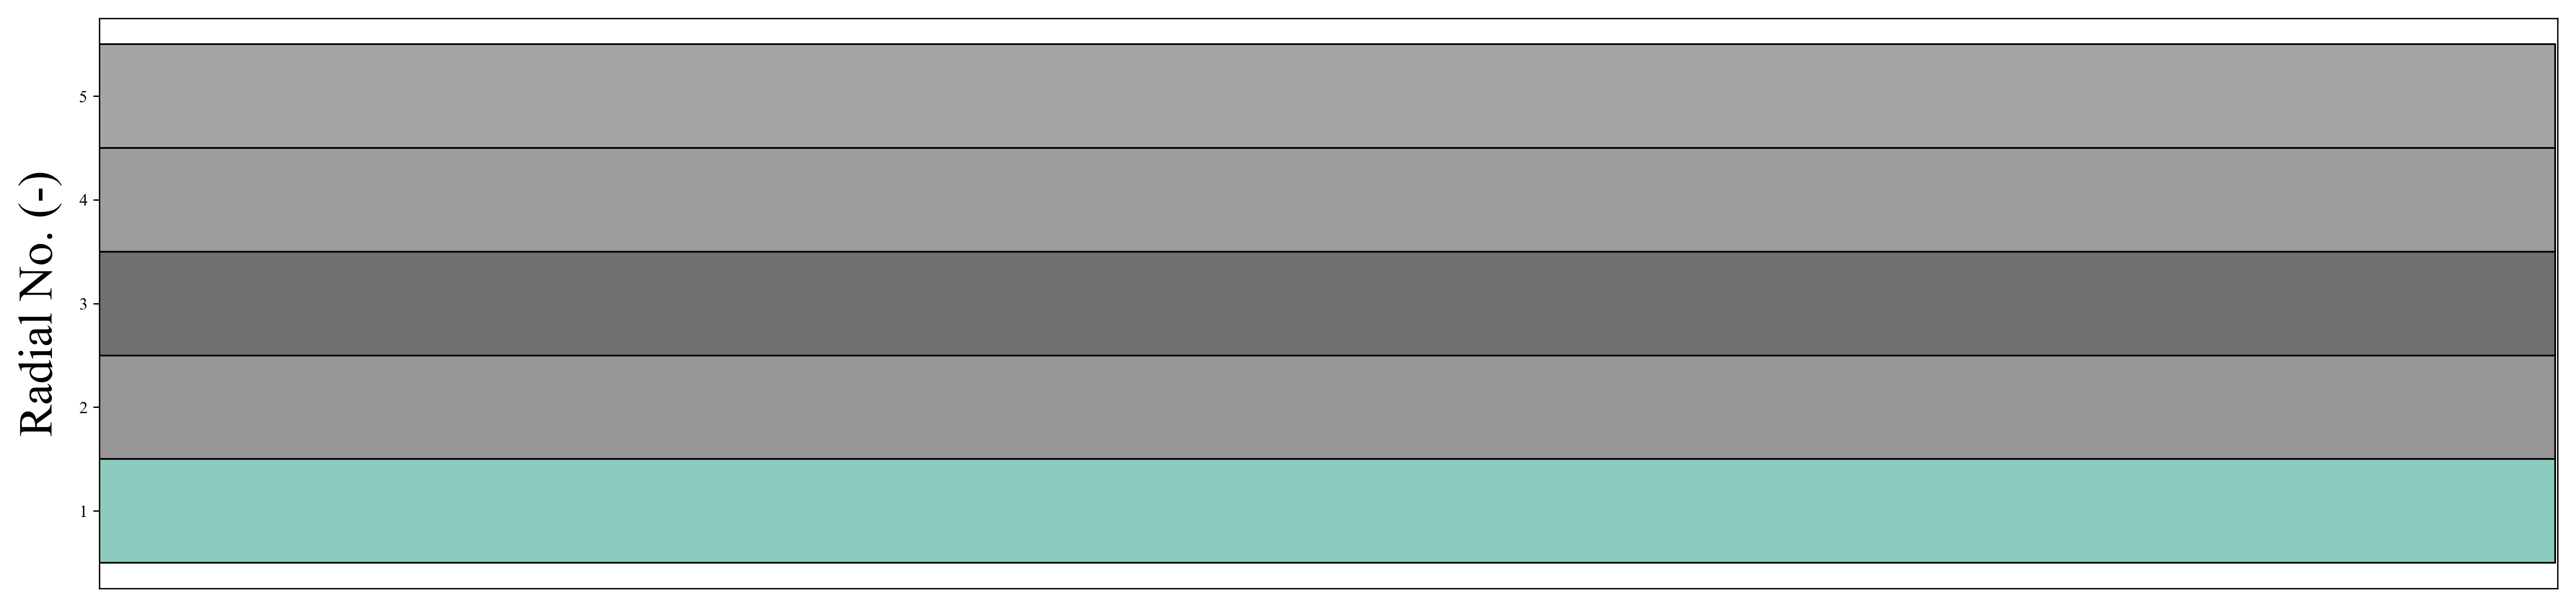
\includegraphics[width=120mm]{results/segments/5seg/50C50T/seg.png}
%\caption{\label{fig:30L6040G1-TField} Strategy I - Segments distribution for 30$^{\rm{th}}$ generation ($w_{\rm{CH_4}} = 0.5, w_T = 0.5$, $T_{\rm{in}}$ = 900 K, $u_{\rm{in}}$ = 0.15 m s$^{-1}$, $SC$ = 2.0)}
%\end{figure}
%
%\begin{figure}[h!]
%\centering
%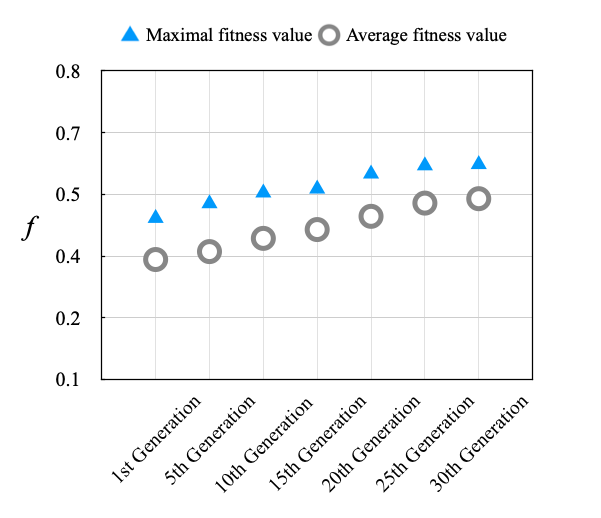
\includegraphics[width=100mm]{results/5/50C_50T.png}
%\caption{\label{fig:5R5050G-fitness} Strategy I - Fitness analysis throughout successive populations ($w_{\rm{CH_4}} = 0.5, w_T = 0.5$, $T_{\rm{in}}$ = 900 K, $u_{\rm{in}}$ = 0.15 m s$^{-1}$, $SC$ = 2.0)}
%\end{figure}
%
%
%\clearpage
%
%
%
%\paragraph{Thermal fitness 40 \%, methane conversion 60 \%} \hspace{0pt} \\
%\noindent 
%
%
%\begin{figure}[h!]
%\centering
%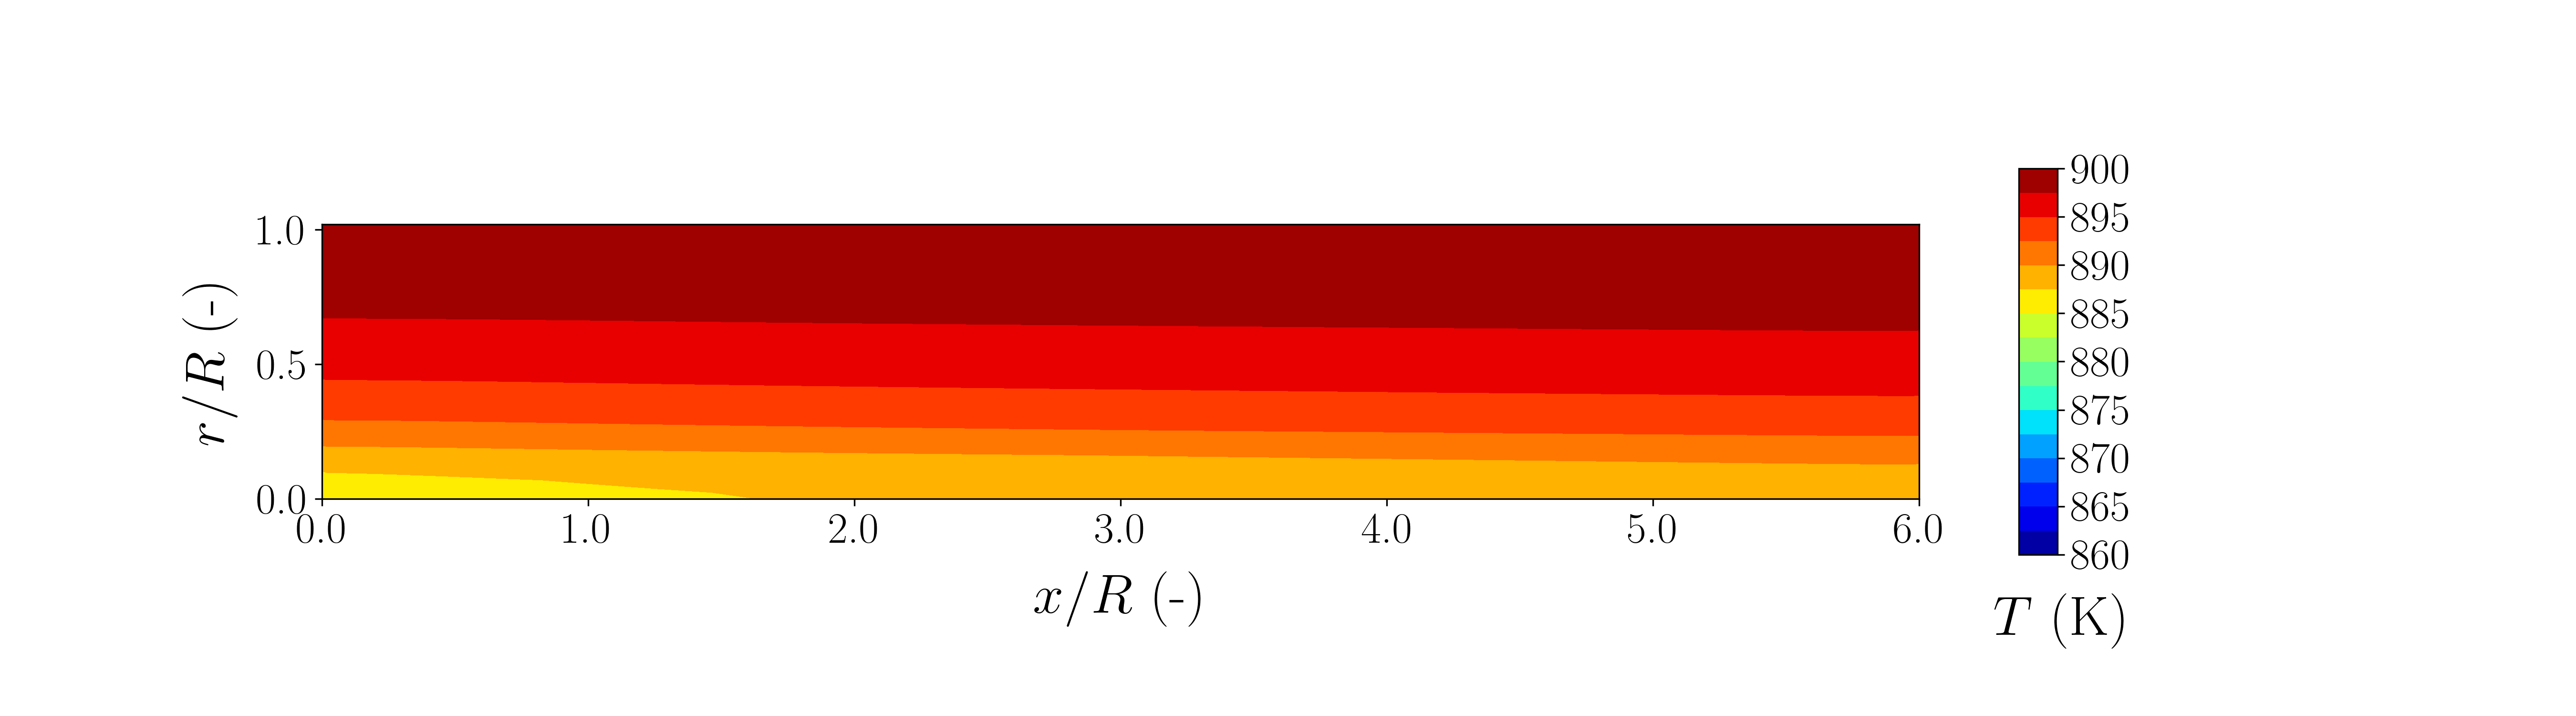
\includegraphics[width=190mm]{results/5/60C_40T/GEN1-TFIELD.png}
%\caption{\label{fig:5R6040G1-TField} Strategy I - Temperature field distribution - 1$^{\rm{st}}$ generation ($w_{\rm{CH_4}} = 0.6, w_T = 0.4$, $T_{\rm{in}}$ = 900 K, $u_{\rm{in}}$ = 0.15 m s$^{-1}$, $SC$ = 2.0)}
%\end{figure}
%
%\begin{figure}[h!]
%\centering
%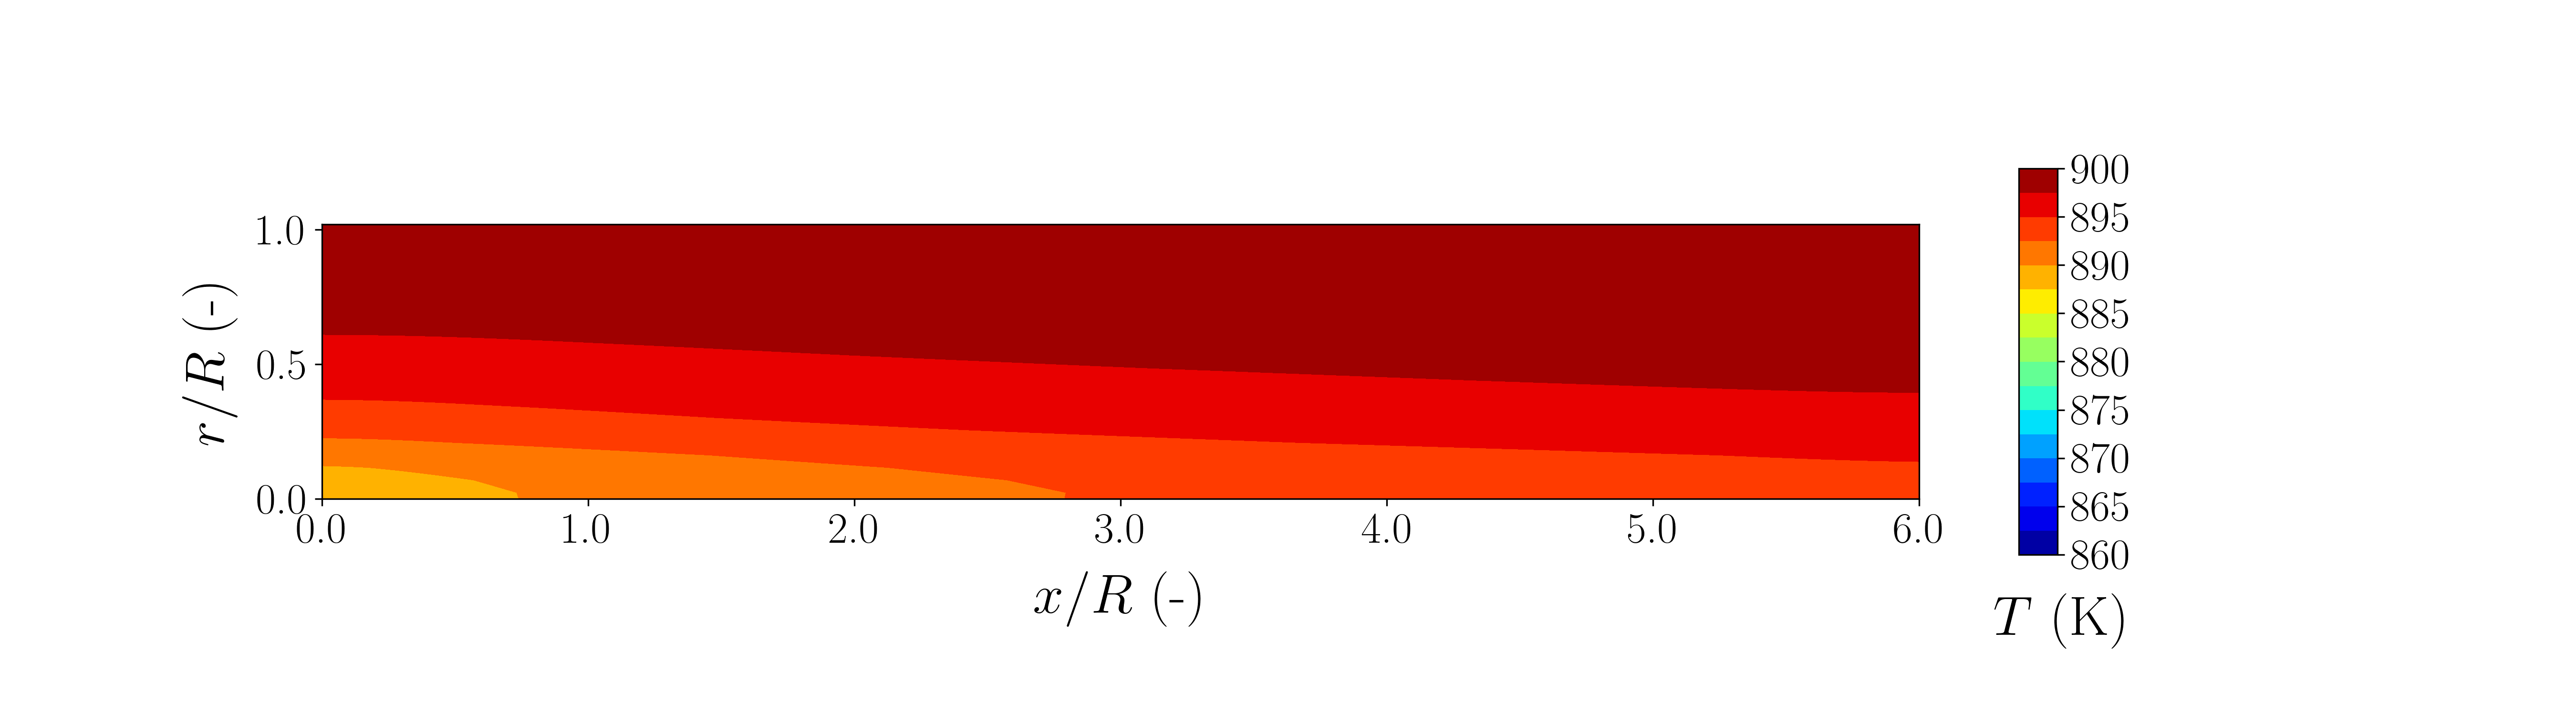
\includegraphics[width=190mm]{results/5/60C_40T/GEN15-TFIELD.png}
%\caption{\label{fig:5R6040G15-TField} Strategy I - Temperature field distribution - 15$^{\rm{th}}$ generation ($w_{\rm{CH_4}} = 0.6, w_T = 0.4$, $T_{\rm{in}}$ = 900 K, $u_{\rm{in}}$ = 0.15 m s$^{-1}$, $SC$ = 2.0)}
%\end{figure}
%
%\begin{figure}[h!]
%\centering
%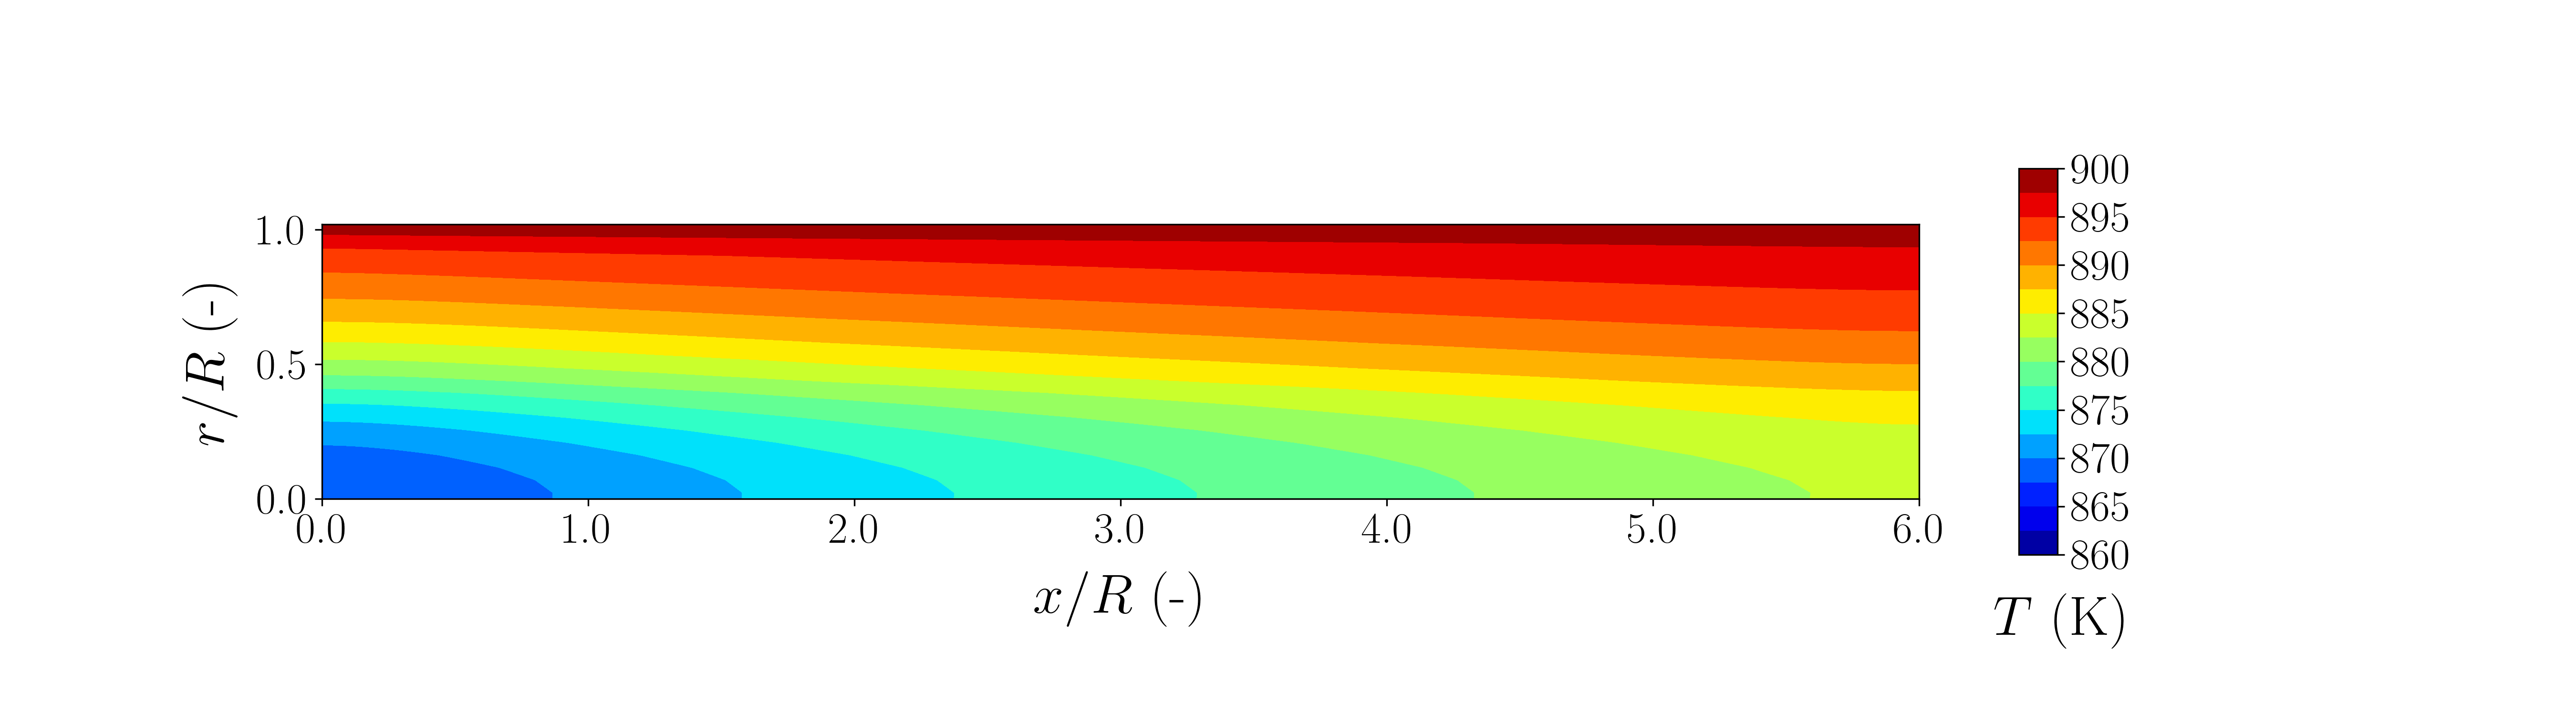
\includegraphics[width=190mm]{results/5/60C_40T/GEN30-TFIELD.png}
%\caption{\label{fig:5R6040G30-TField} Strategy I - Temperature field distribution - 30$^{\rm{th}}$ generation ($w_{\rm{CH_4}} = 0.6, w_T = 0.4$, $T_{\rm{in}}$ = 900 K, $u_{\rm{in}}$ = 0.15 m s$^{-1}$, $SC$ = 2.0)}
%\end{figure}
%
%
%\begin{figure}[h!]
%\centering
%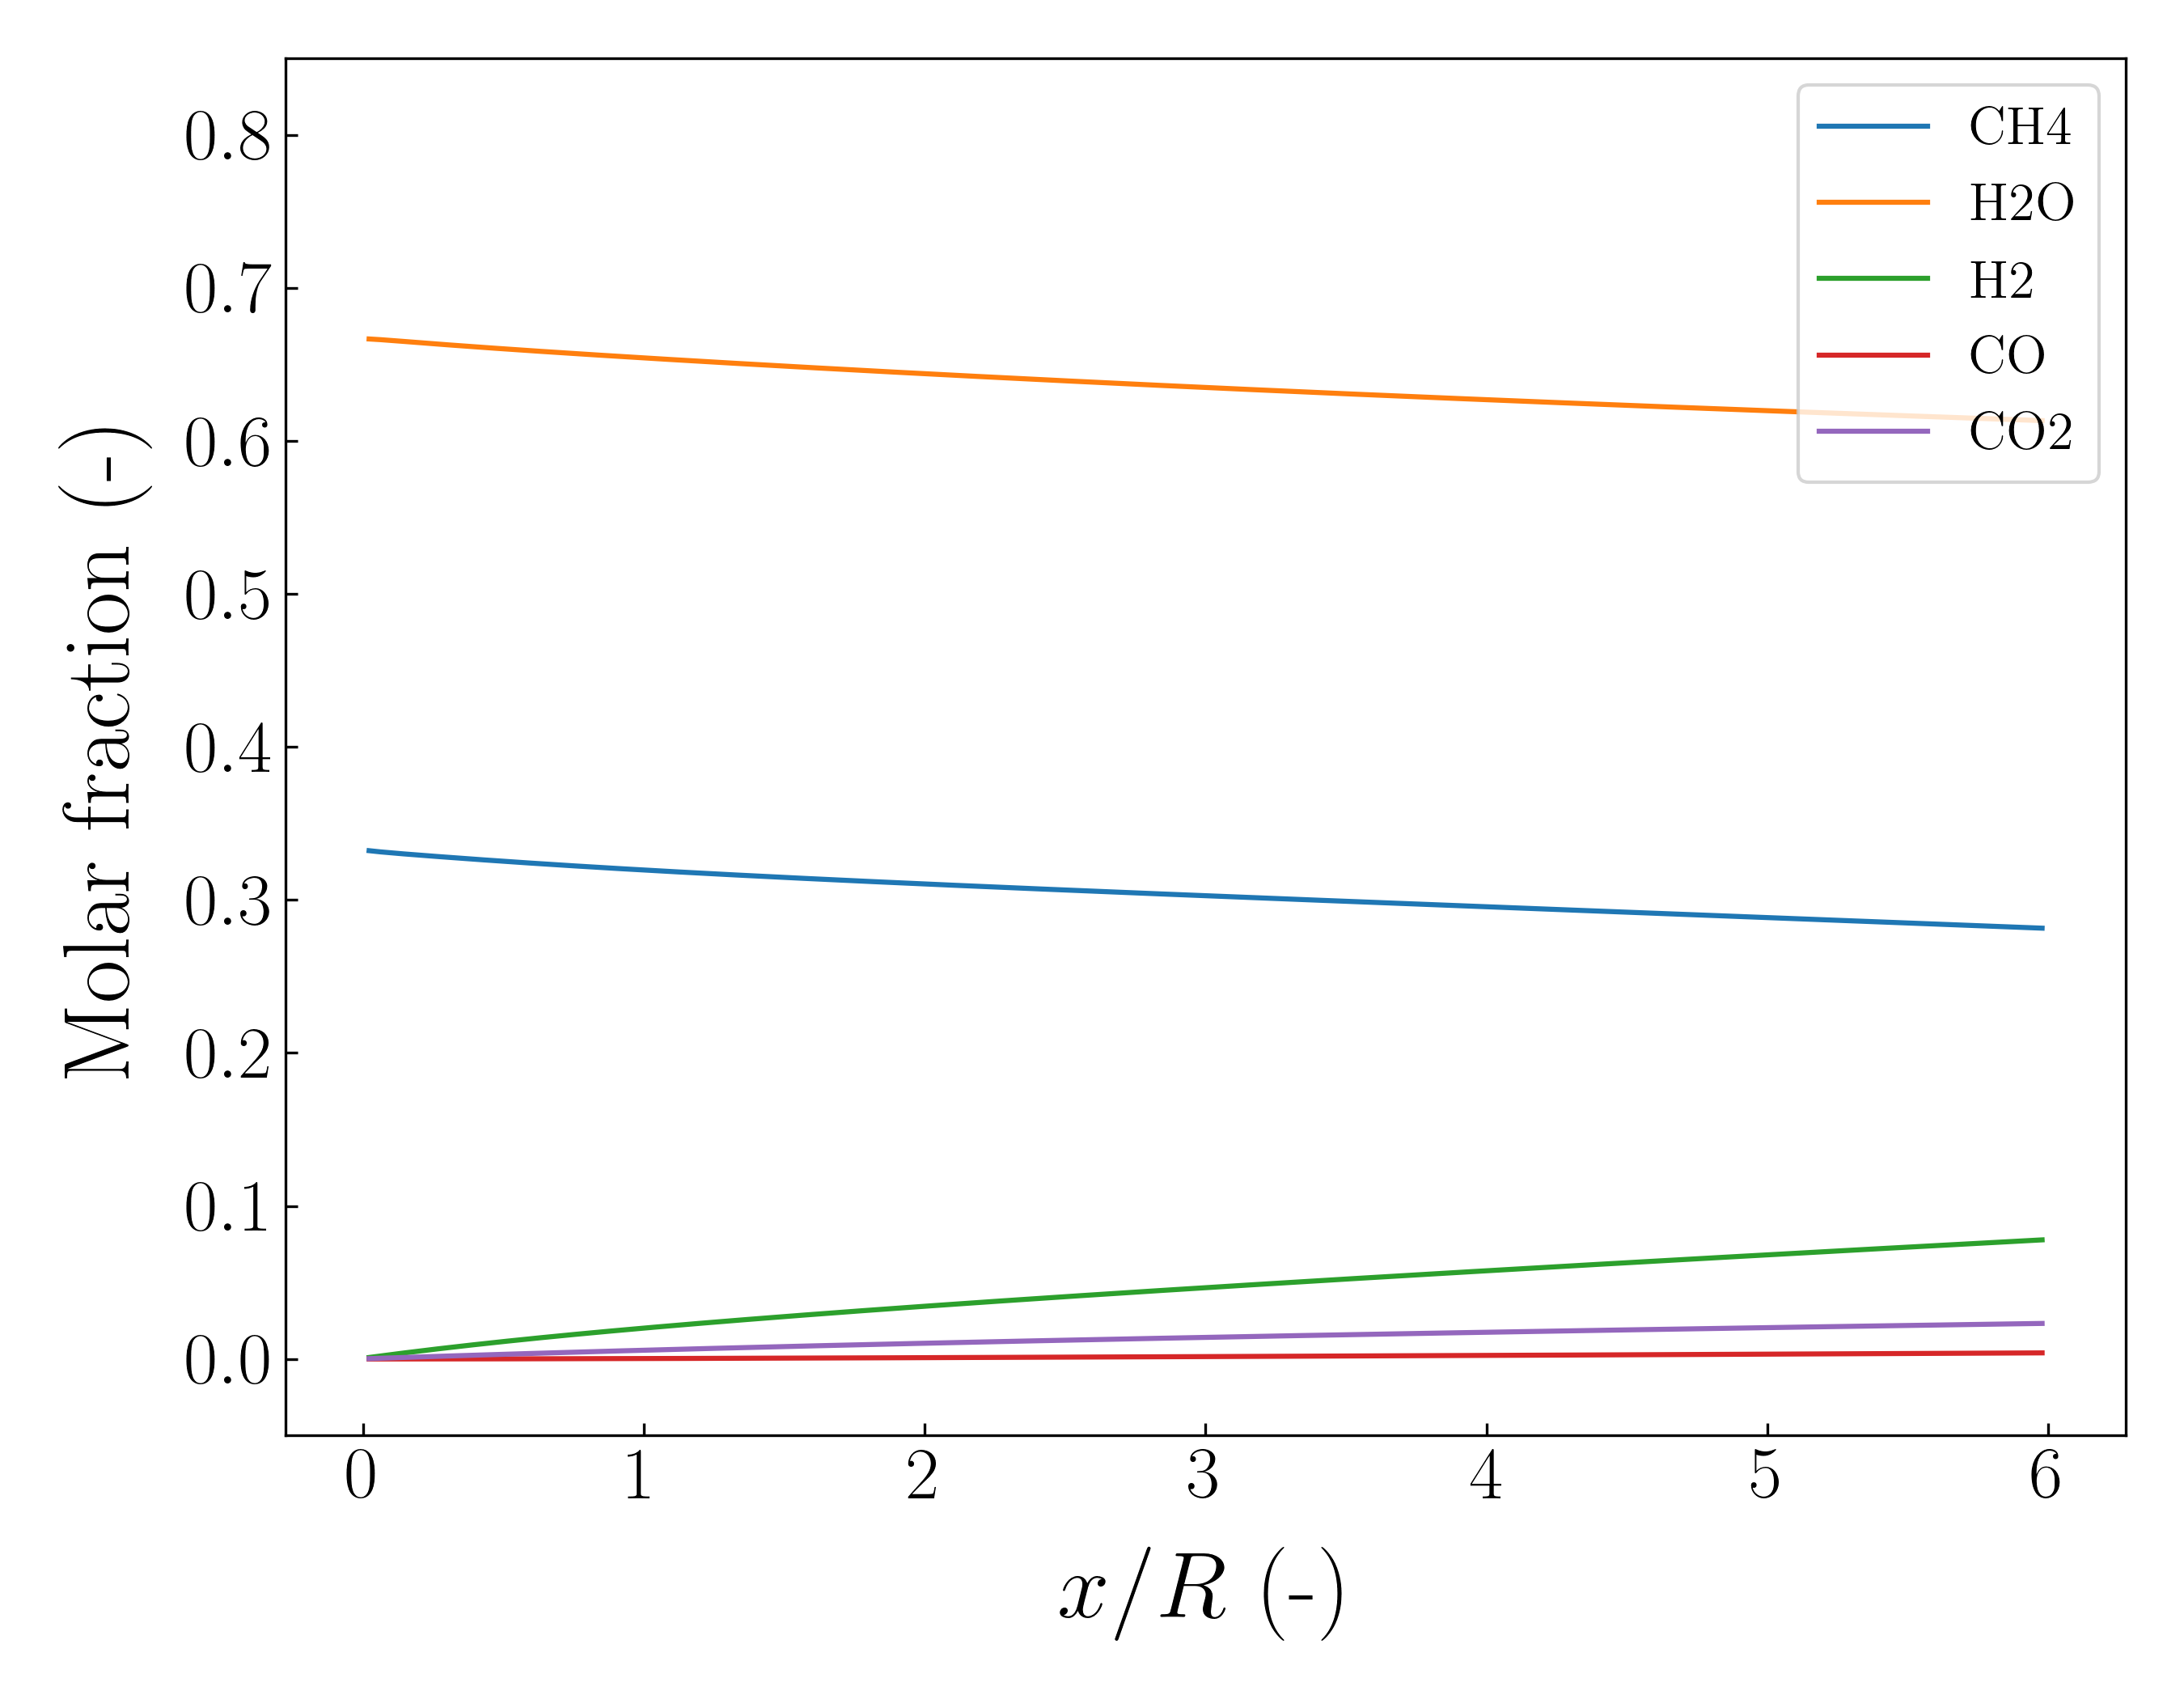
\includegraphics[width=80mm]{results/5/60C_40T/GEN1-AVG.png}
%\caption{\label{fig:5R6040G1-avg} Strategy I - Radius-averaged molar fractions - 1$^{\rm{st}}$ generation ($w_{\rm{CH_4}} = 0.6, w_T = 0.4$, $T_{\rm{in}}$ = 900 K, $u_{\rm{in}}$ = 0.15 m s$^{-1}$, $SC$ = 2.0)}
%\end{figure}
%
%\begin{figure}[h!]
%\centering
%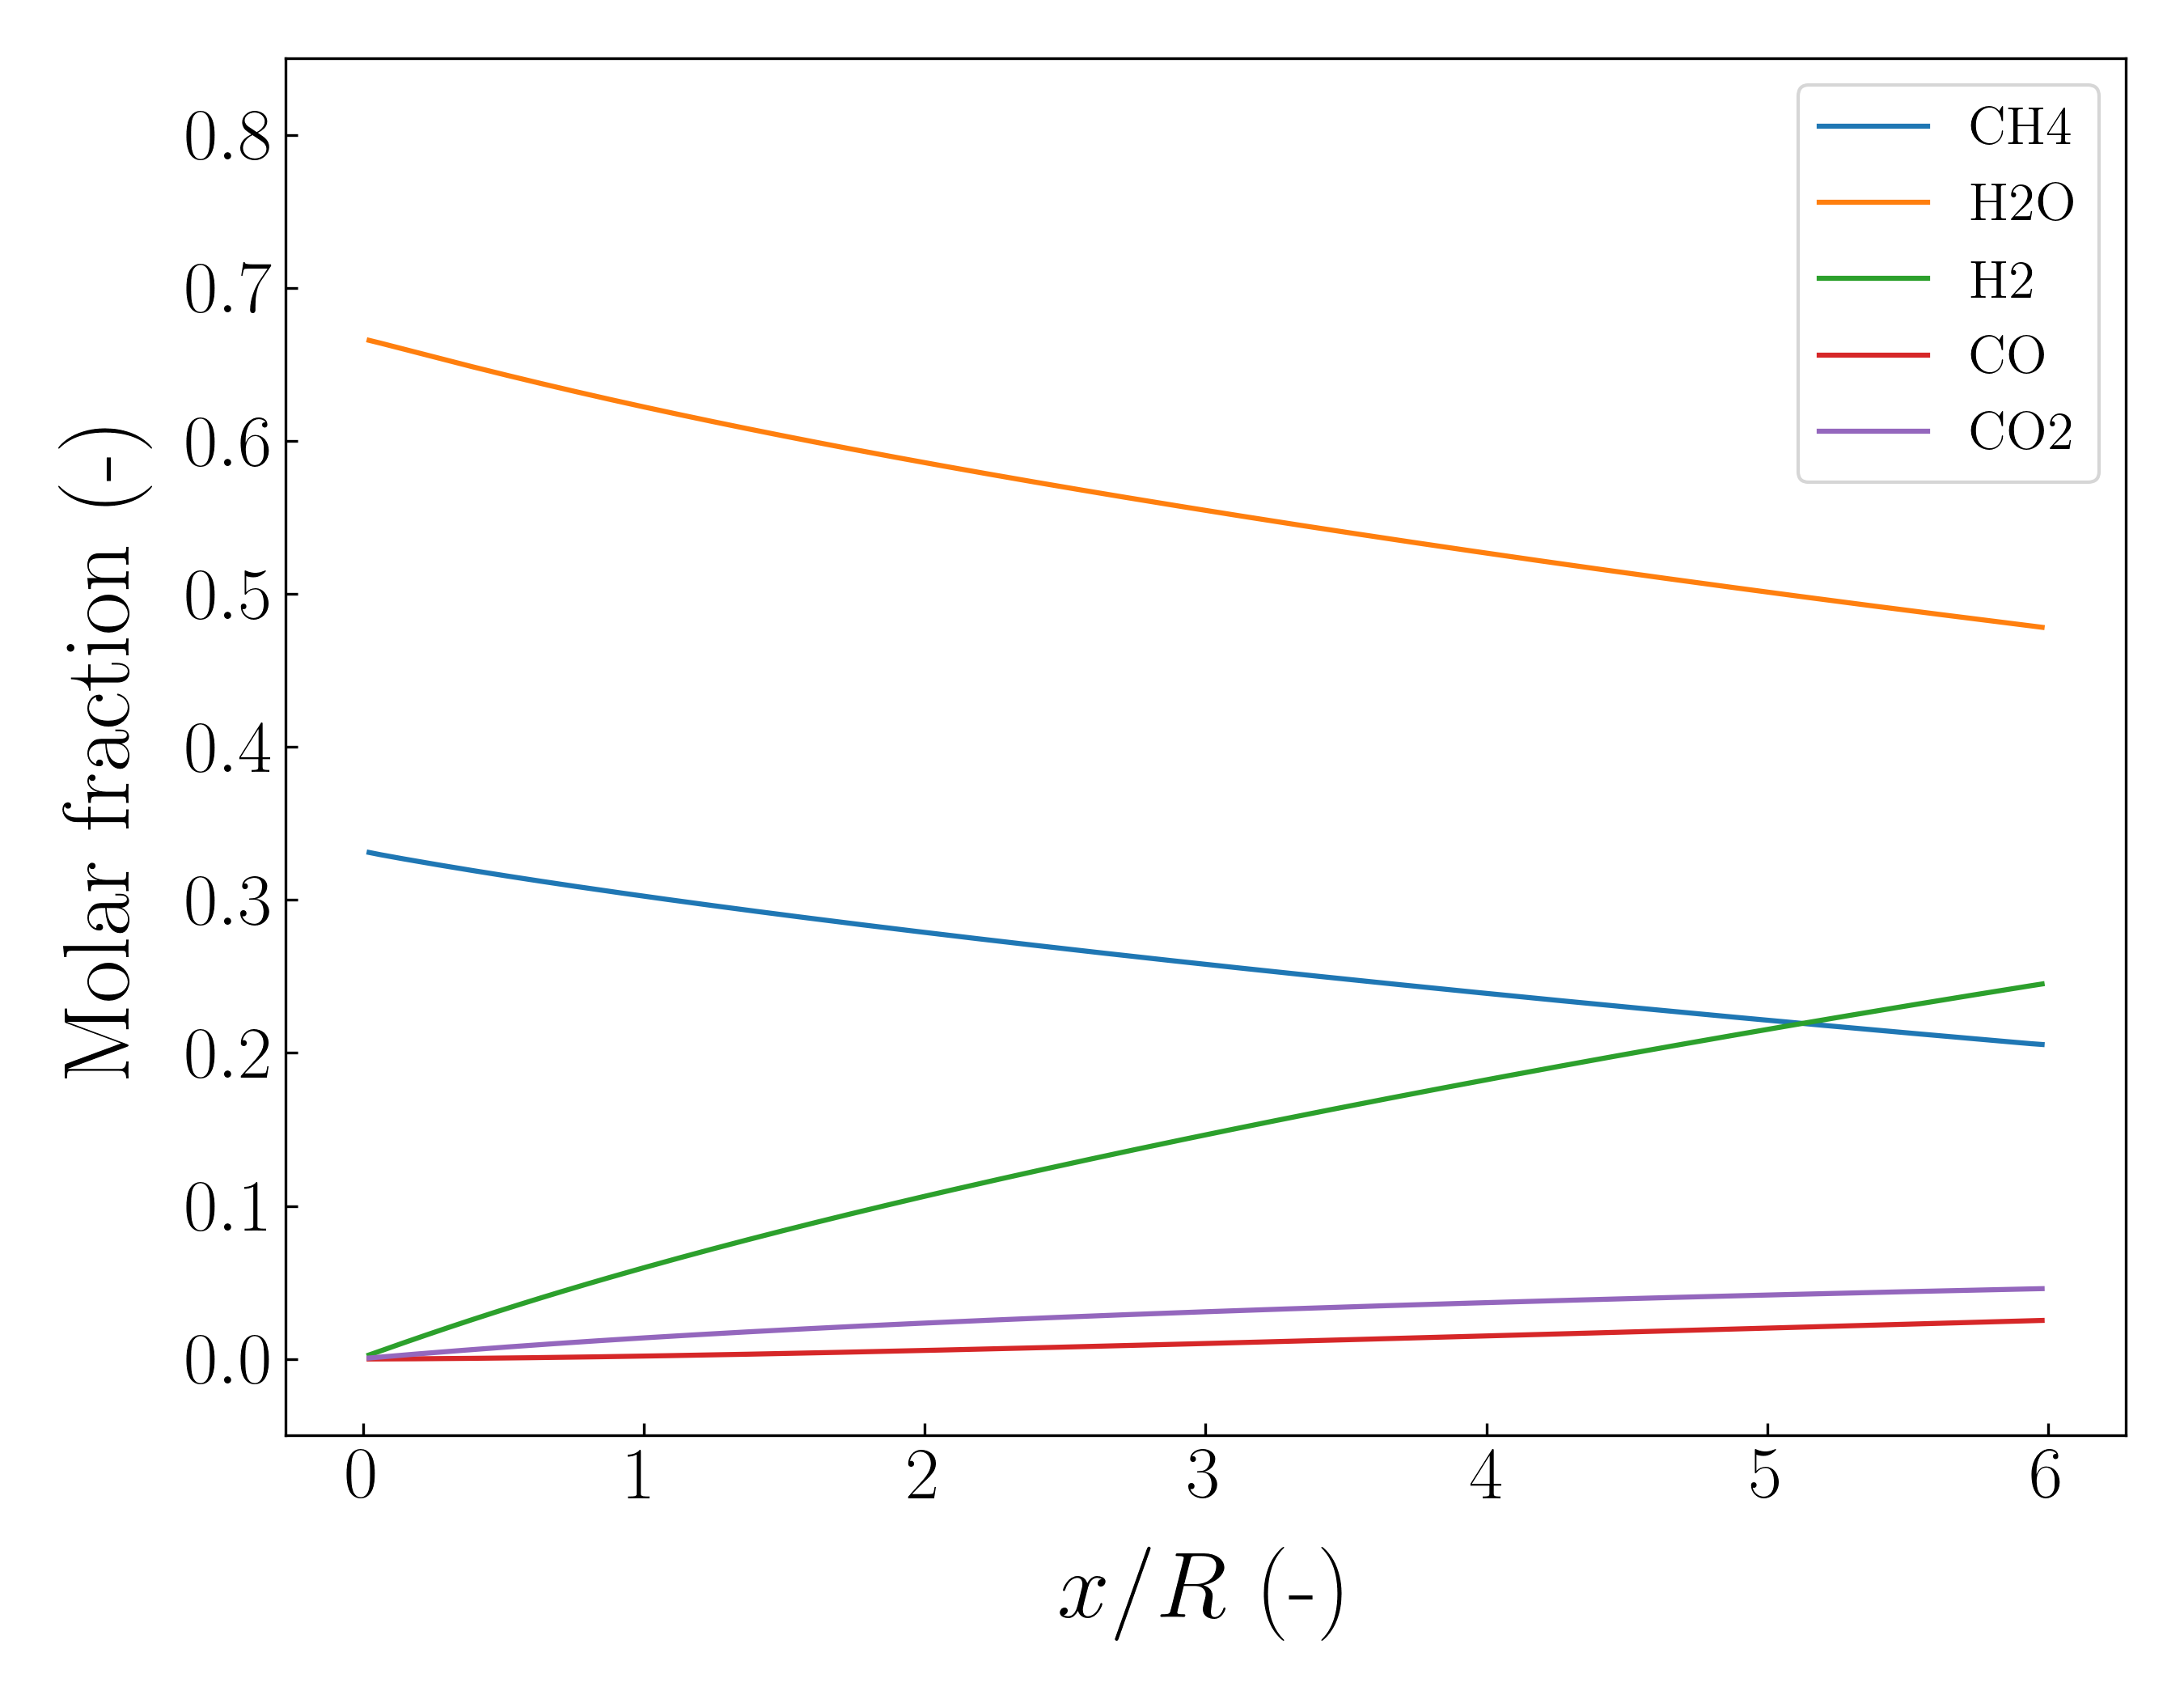
\includegraphics[width=80mm]{results/5/60C_40T/GEN15-AVG.png}
%\caption{\label{fig:5R6040G15-avg} Strategy I - Radius-averaged molar fractions - 15$^{\rm{th}}$ generation ($w_{\rm{CH_4}} = 0.6, w_T = 0.4$, $T_{\rm{in}}$ = 900 K, $u_{\rm{in}}$ = 0.15 m s$^{-1}$, $SC$ = 2.0)}
%\end{figure}
%
%\begin{figure}[h!]
%\centering
%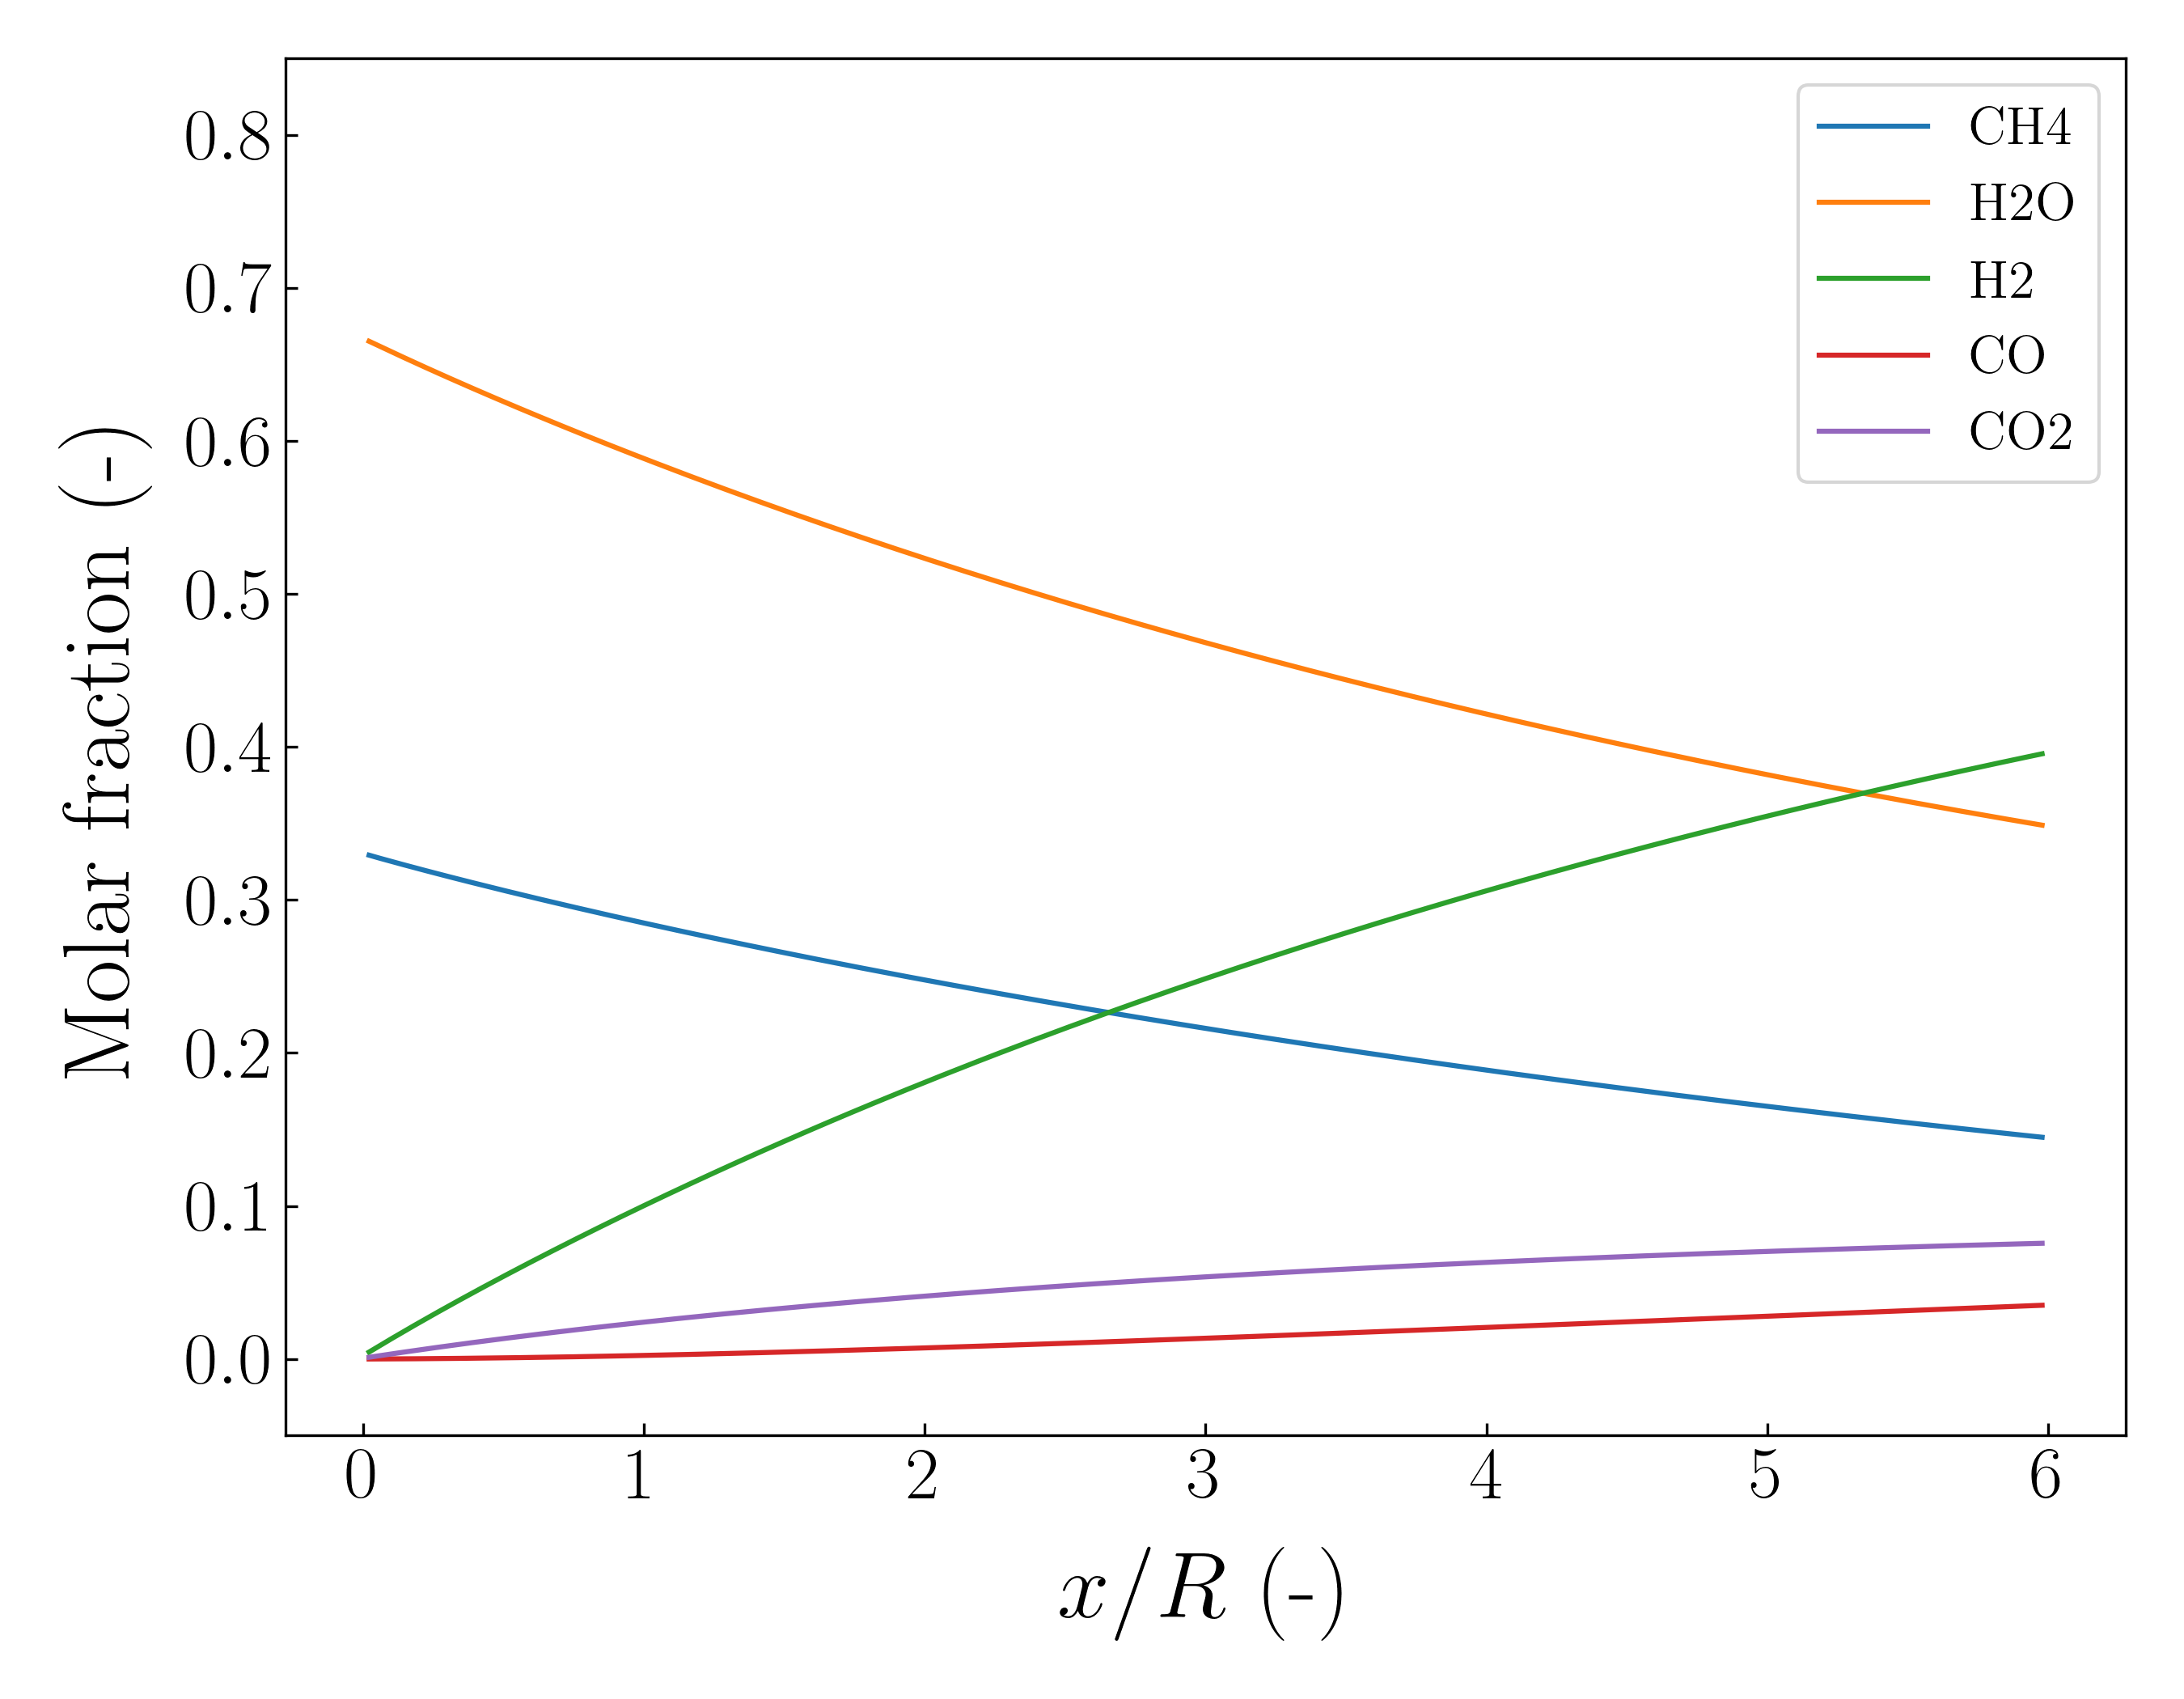
\includegraphics[width=80mm]{results/5/60C_40T/GEN30-AVG.png}
%\caption{\label{fig:5R6040G30-avg} Strategy I - Radius-averaged molar fractions -  30$^{\rm{th}}$ generation ($w_{\rm{CH_4}} = 0.6, w_T = 0.4$, $T_{\rm{in}}$ = 900 K, $u_{\rm{in}}$ = 0.15 m s$^{-1}$, $SC$ = 2.0)}
%\end{figure}
%
%\begin{figure}[h!]
%\centering
%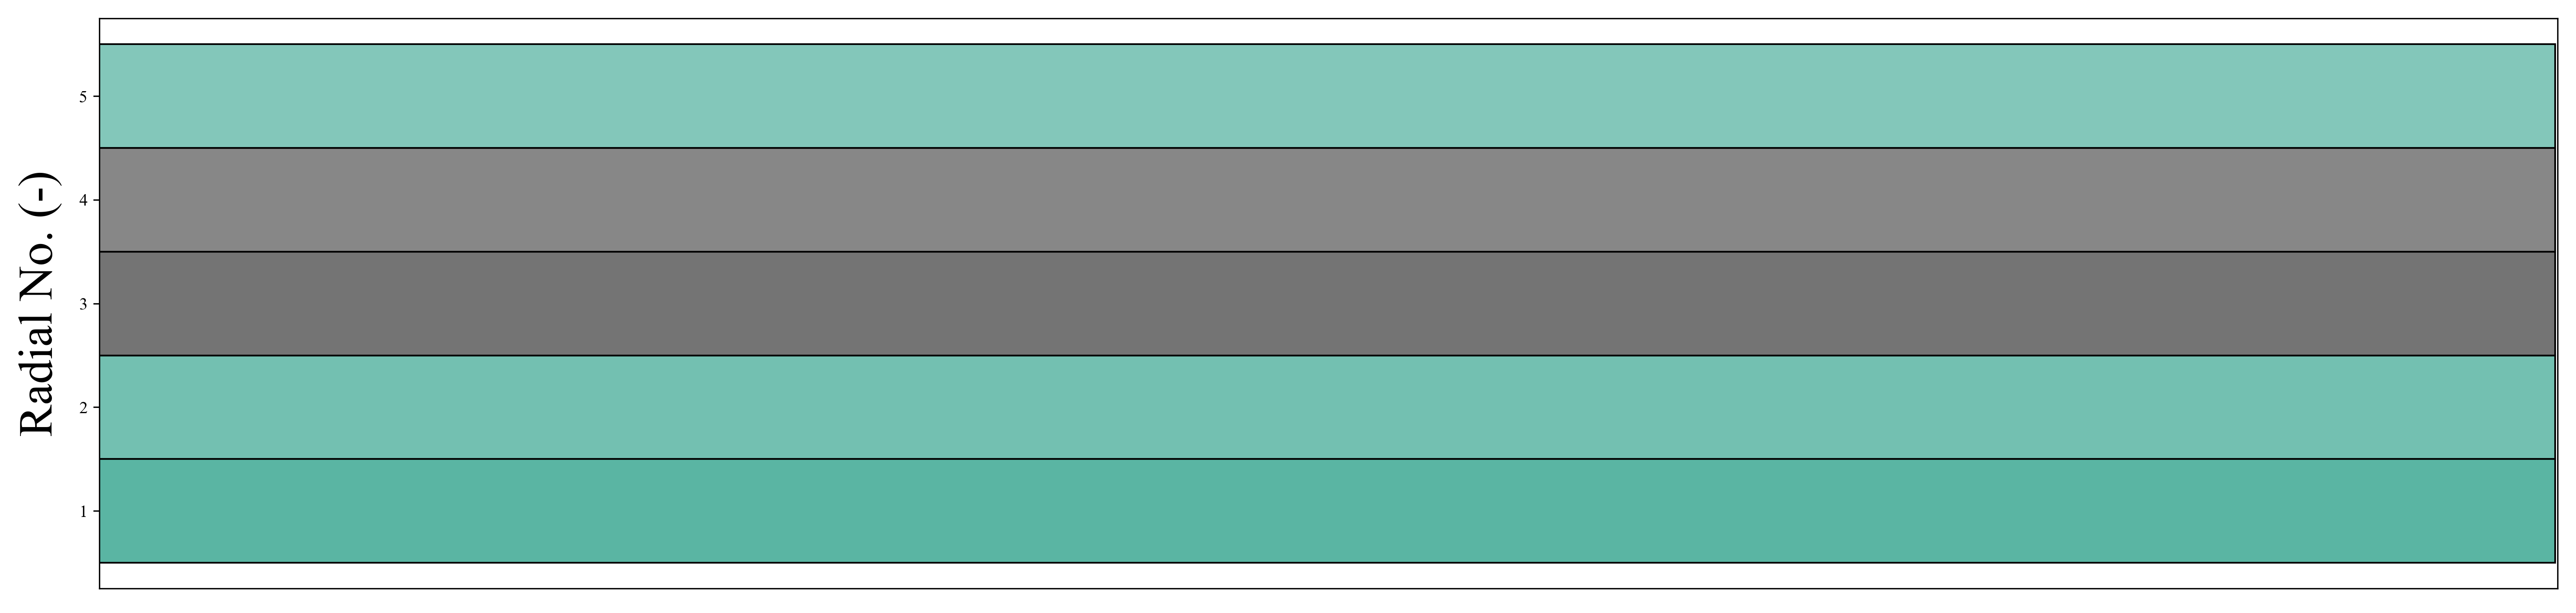
\includegraphics[width=120mm]{results/segments/5seg/60C40T/seg.png}
%\caption{\label{fig:30L6040G1-TField} Strategy I - Segments distribution for 30$^{\rm{th}}$ generation ($w_{\rm{CH_4}} = 0.6, w_T = 0.4$, $T_{\rm{in}}$ = 900 K, $u_{\rm{in}}$ = 0.15 m s$^{-1}$, $SC$ = 2.0)}
%\end{figure}
%
%\begin{figure}[h!]
%\centering
%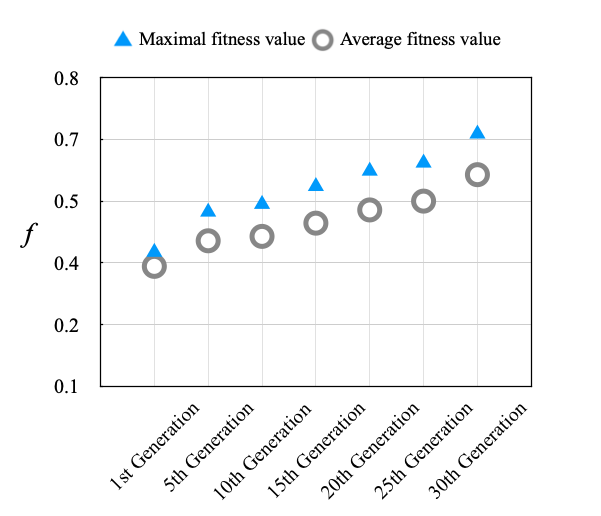
\includegraphics[width=100mm]{results/5/60C_40T.png}
%\caption{\label{fig:5R6040G-fitness} Strategy I - Fitness analysis throughout successive populations ($w_{\rm{CH_4}} = 0.6, w_T = 0.4$, $T_{\rm{in}}$ = 900 K, $u_{\rm{in}}$ = 0.15 m s$^{-1}$, $SC$ = 2.0)}
%\end{figure}
%
%\clearpage
%
%
%\paragraph{Thermal fitness 20 \%, methane conversion 80 \%} \hspace{0pt} \\
%\noindent 
%
%
%
%\begin{figure}[h!]
%\centering
%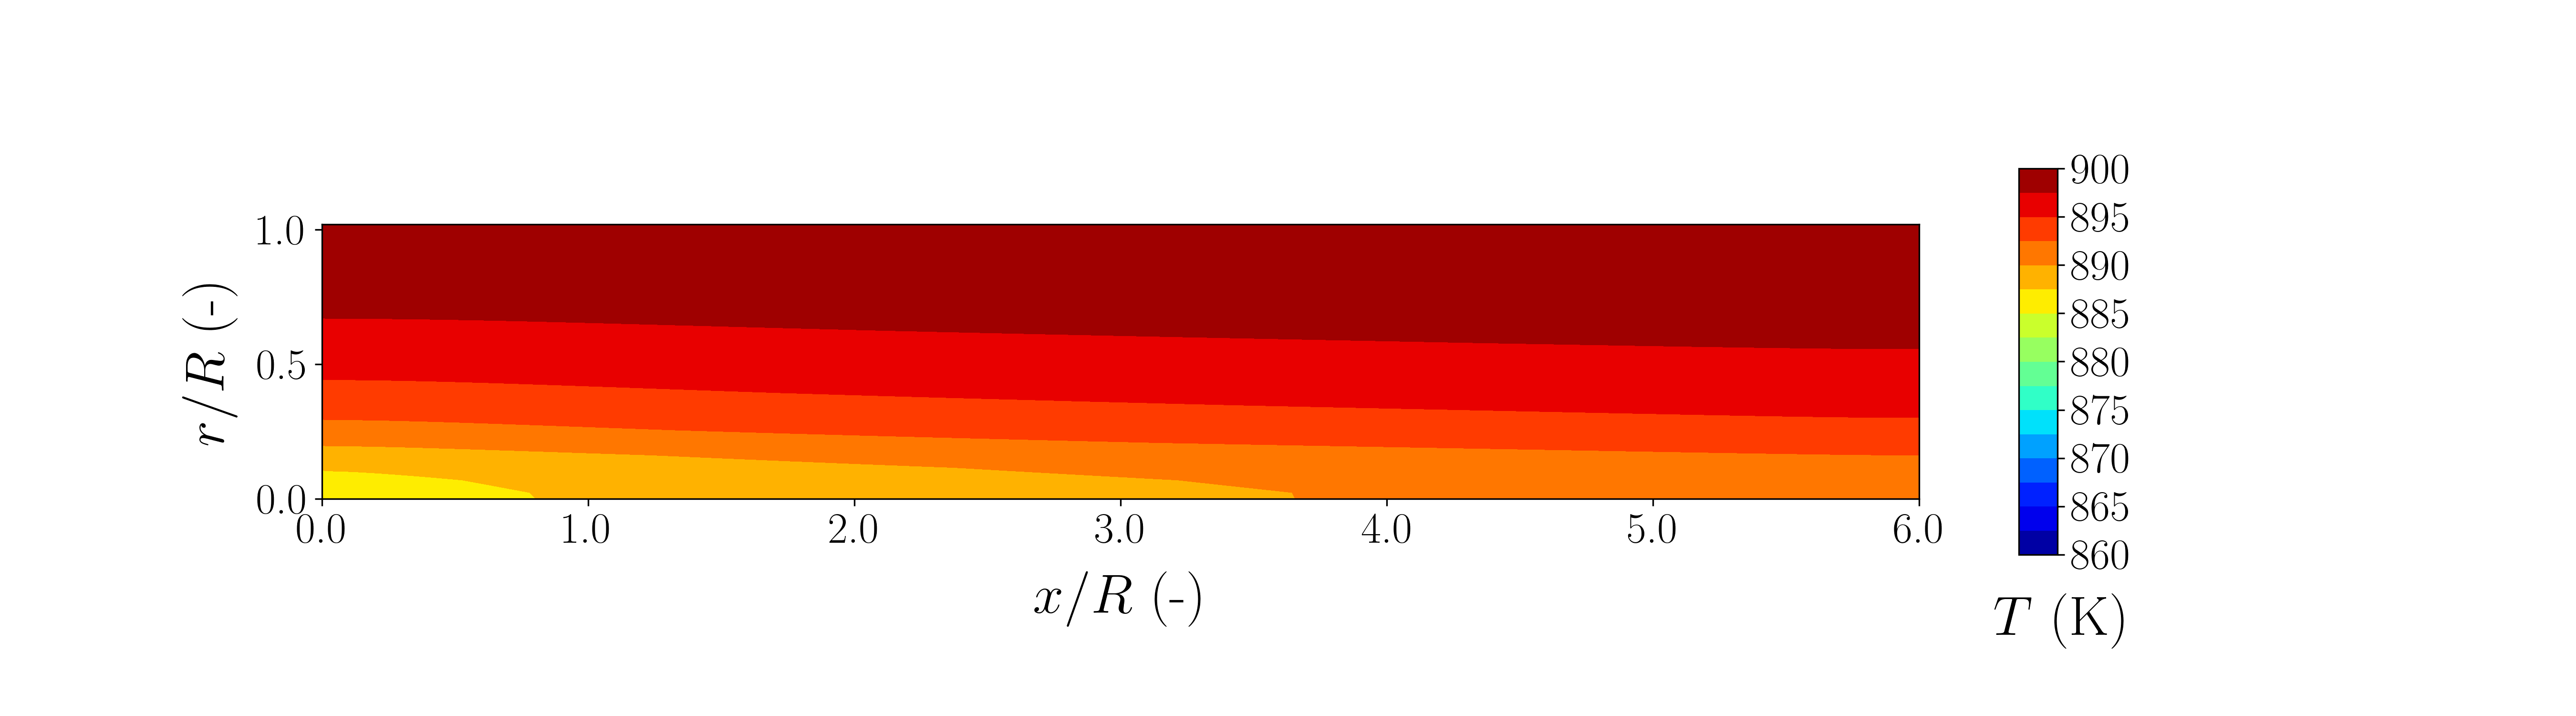
\includegraphics[width=190mm]{results/5/80C_20T/GEN1-TFIELD.png}
%\caption{\label{fig:5R8020G1-TField} Strategy I - Temperature field distribution - 1$^{\rm{st}}$ generation ($w_{\rm{CH_4}} = 0.8, w_T = 0.2$, $T_{\rm{in}}$ = 900 K, $u_{\rm{in}}$ = 0.15 m s$^{-1}$, $SC$ = 2.0)}
%\end{figure}
%
%\begin{figure}[h!]
%\centering
%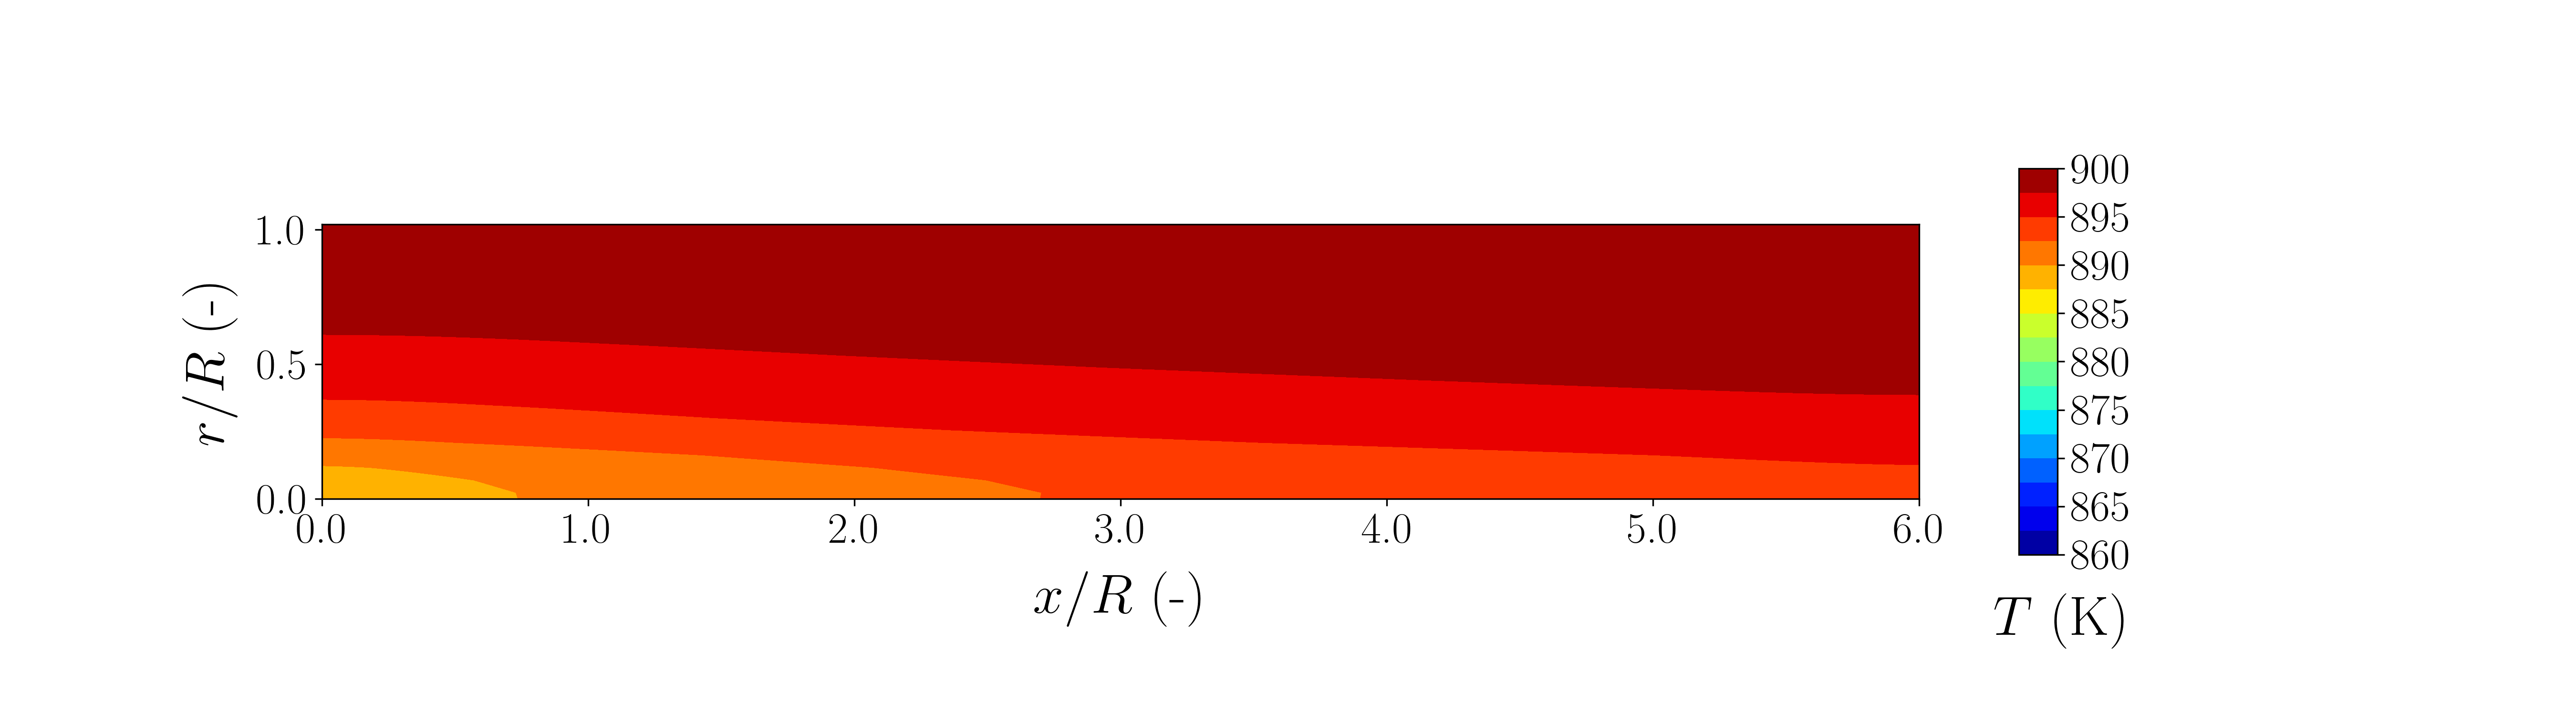
\includegraphics[width=190mm]{results/5/80C_20T/GEN15-TFIELD.png}
%\caption{\label{fig:5R8020G15-TField} Strategy I - Temperature field distribution - 15$^{\rm{th}}$ generation ($w_{\rm{CH_4}} = 0.8, w_T = 0.2$, $T_{\rm{in}}$ = 900 K, $u_{\rm{in}}$ = 0.15 m s$^{-1}$, $SC$ = 2.0)}
%\end{figure}
%
%\begin{figure}[h!]
%\centering
%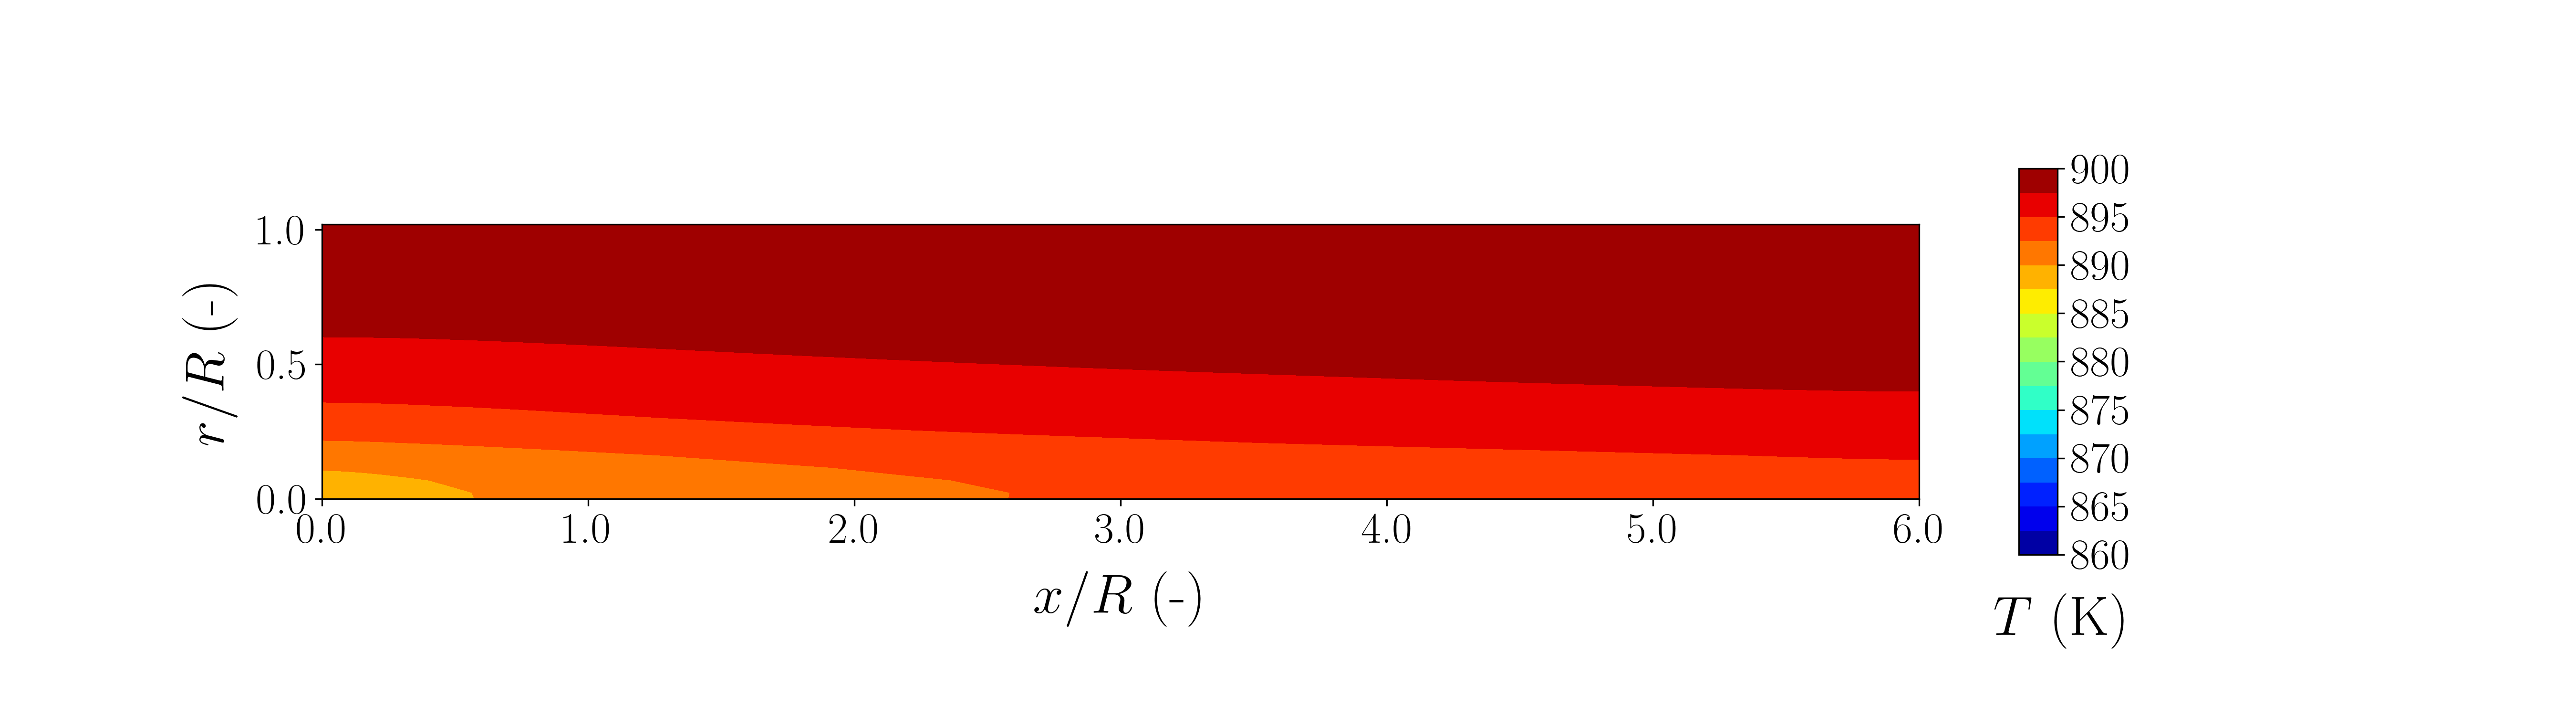
\includegraphics[width=190mm]{results/5/80C_20T/GEN30-TFIELD.png}
%\caption{\label{fig:5R8020G30-TField} Strategy I - Temperature field distribution - 30$^{\rm{th}}$ generation ($w_{\rm{CH_4}} = 0.8, w_T = 0.2$, $T_{\rm{in}}$ = 900 K, $u_{\rm{in}}$ = 0.15 m s$^{-1}$, $SC$ = 2.0)}
%\end{figure}
%
%
%\begin{figure}[h!]
%\centering
%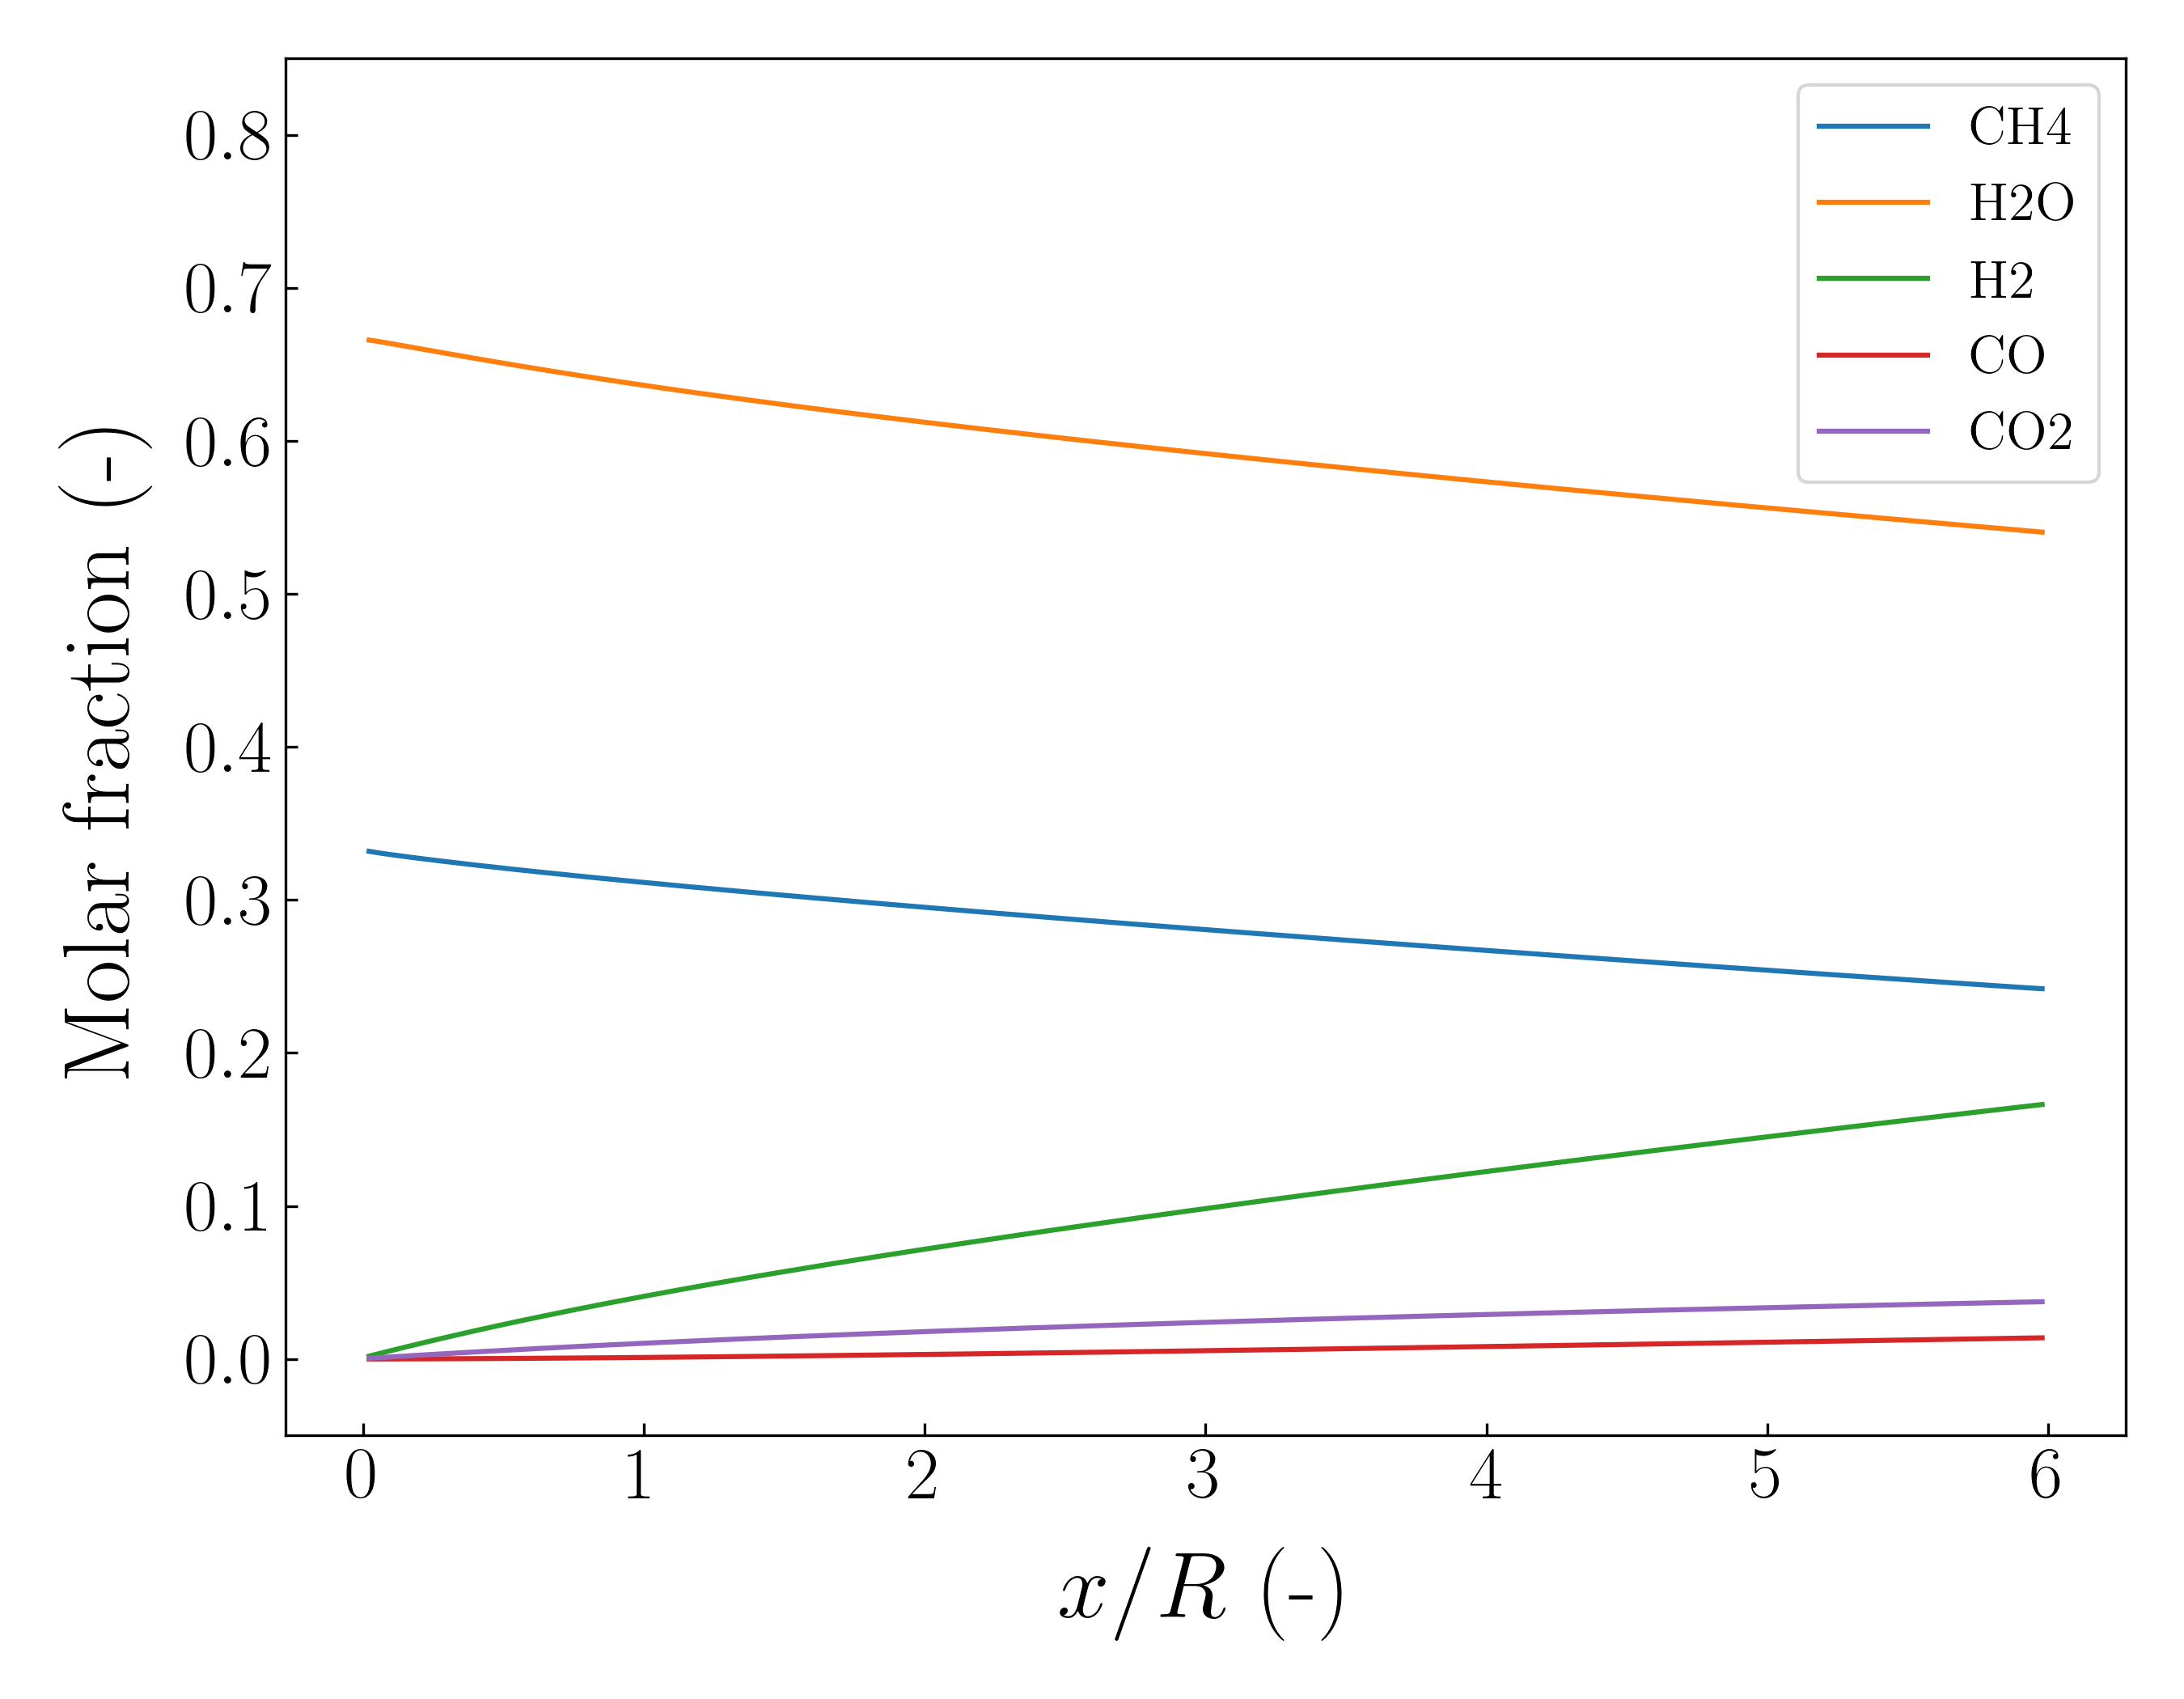
\includegraphics[width=80mm]{results/5/80C_20T/GEN1-AVG.png}
%\caption{\label{fig:5R8020G1-avg} Strategy I - Radius-averaged molar fractions - 1$^{\rm{st}}$ generation ($w_{\rm{CH_4}} = 0.8, w_T = 0.2$, $T_{\rm{in}}$ = 900 K, $u_{\rm{in}}$ = 0.15 m s$^{-1}$, $SC$ = 2.0)}
%\end{figure}
%
%\begin{figure}[h!]
%\centering
%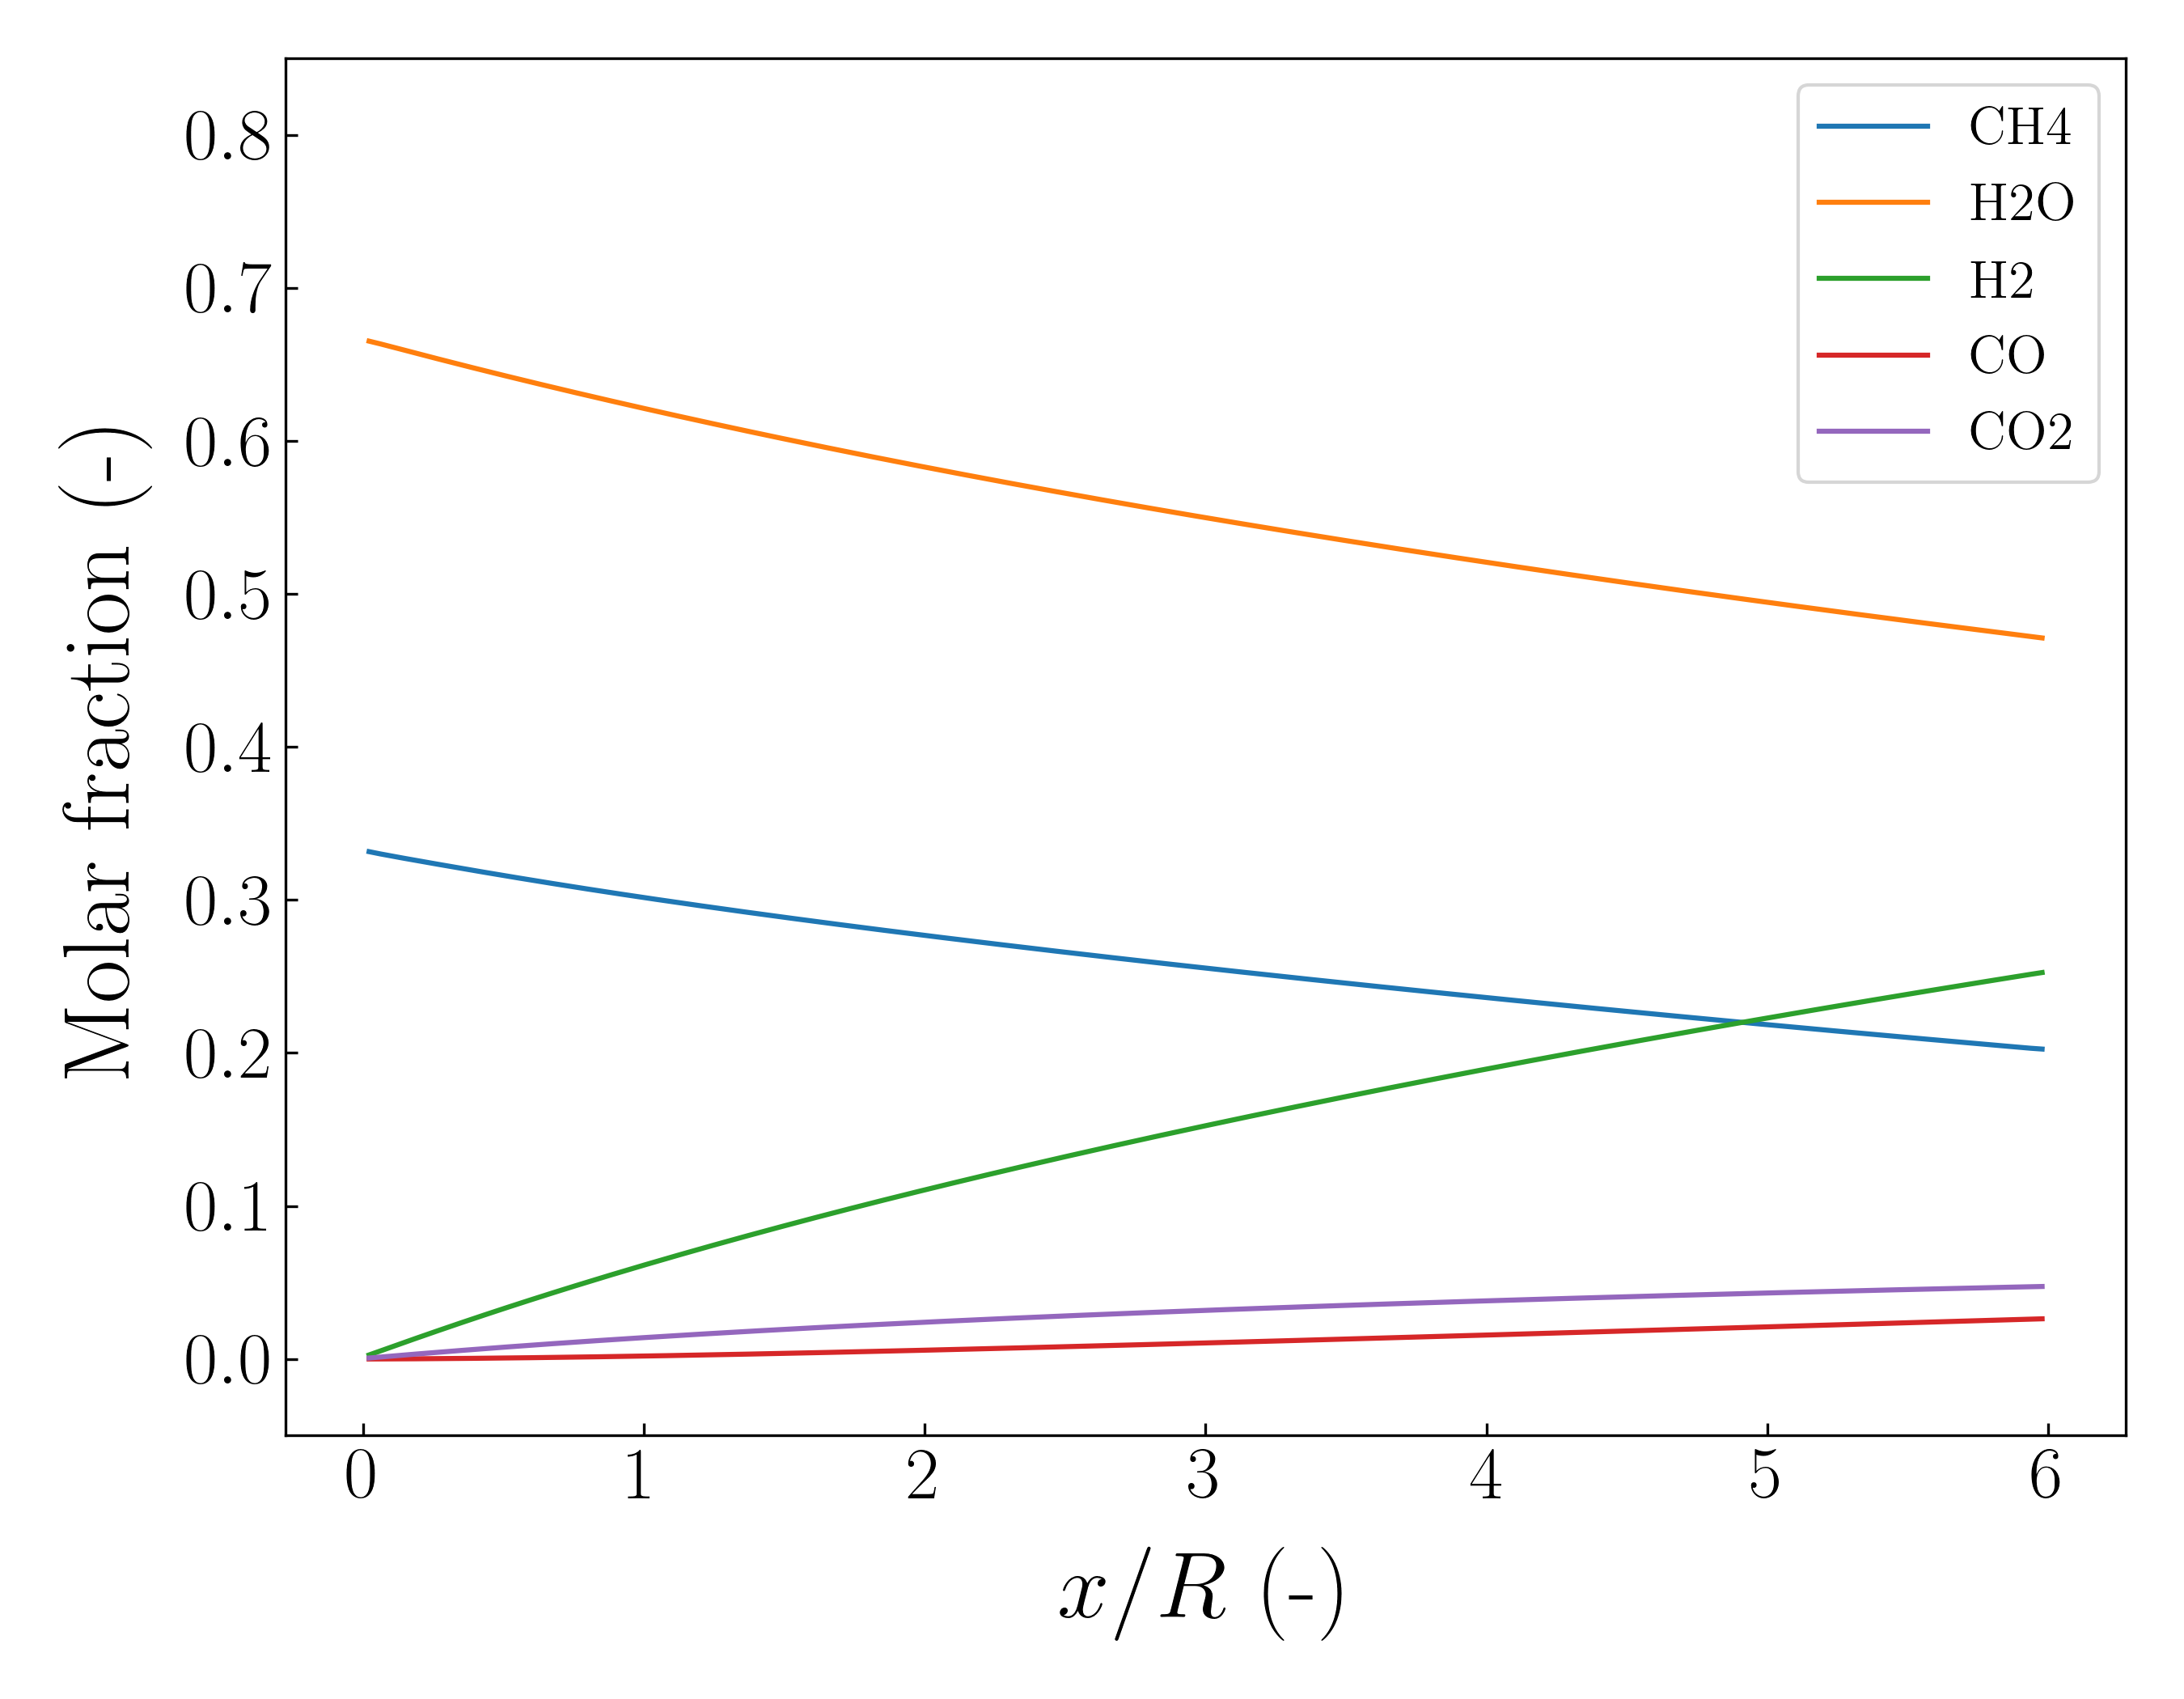
\includegraphics[width=80mm]{results/5/80C_20T/GEN15-AVG.png}
%\caption{\label{fig:5R8020G15-avg} Strategy I - Radius-averaged molar fractions - 15$^{\rm{th}}$ generation ($w_{\rm{CH_4}} = 0.8, w_T = 0.2$, $T_{\rm{in}}$ = 900 K, $u_{\rm{in}}$ = 0.15 m s$^{-1}$, $SC$ = 2.0)}
%\end{figure}
%
%\begin{figure}[h!]
%\centering
%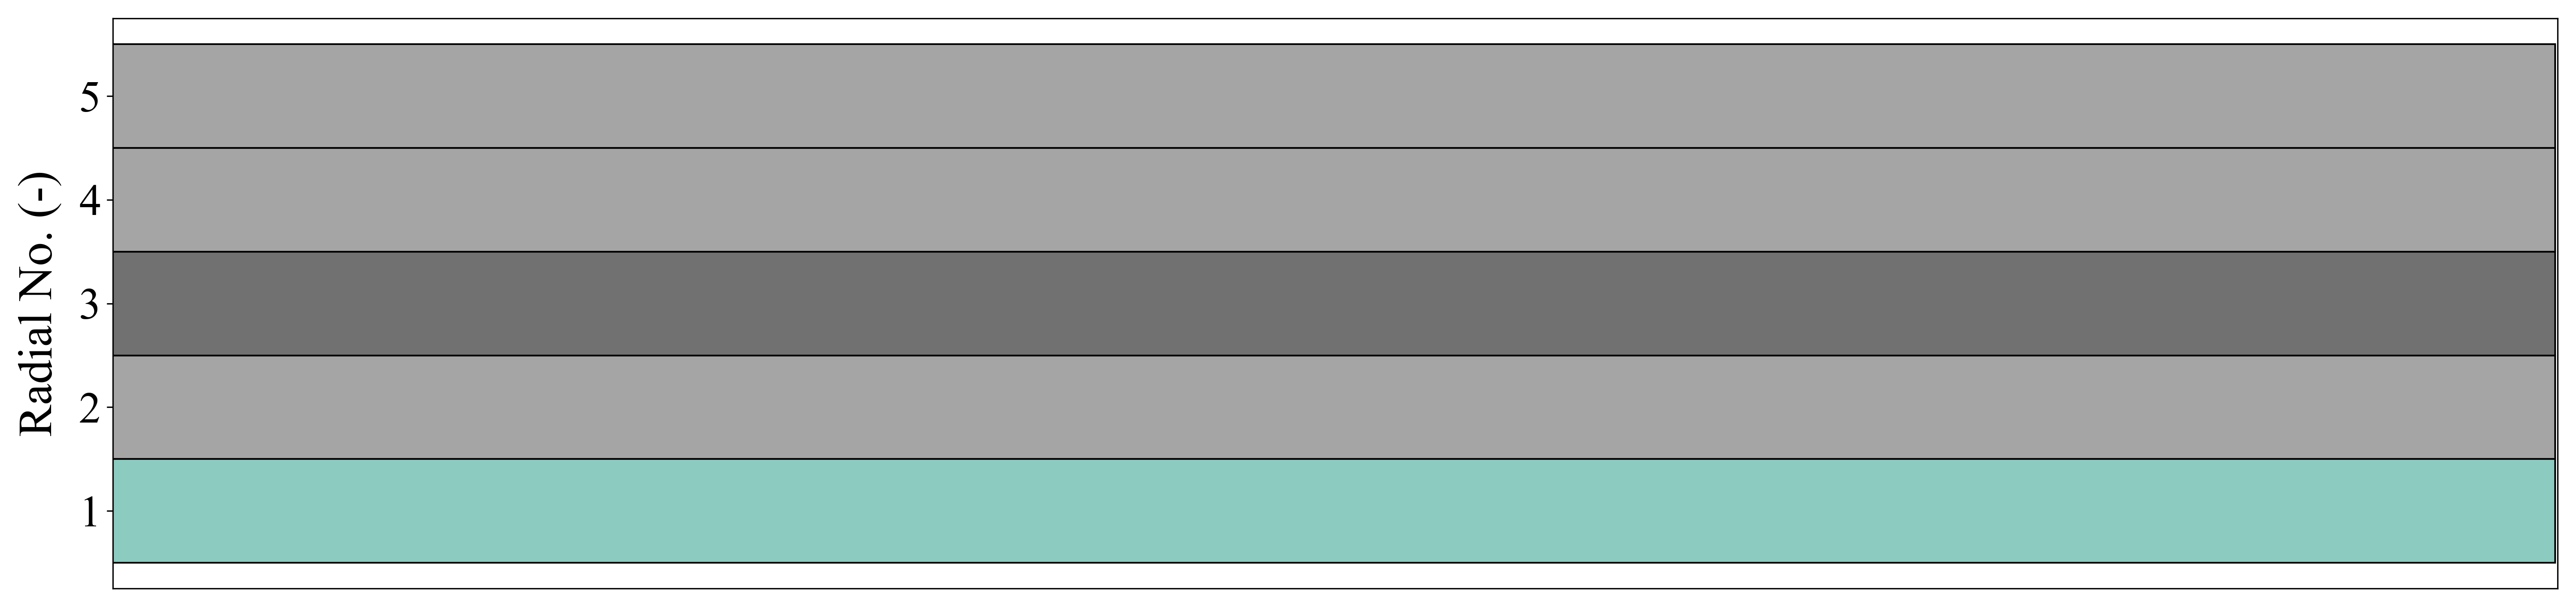
\includegraphics[width=120mm]{results/segments/5seg/80C20T/seg.png}
%\caption{\label{fig:30L6040G1-TField} Strategy I - Segments distribution for 30$^{\rm{th}}$ generation ($w_{\rm{CH_4}} = 0.8, w_T = 0.2$, $T_{\rm{in}}$ = 900 K, $u_{\rm{in}}$ = 0.15 m s$^{-1}$, $SC$ = 2.0)}
%\end{figure}
%
%\begin{figure}[h!]
%\centering
%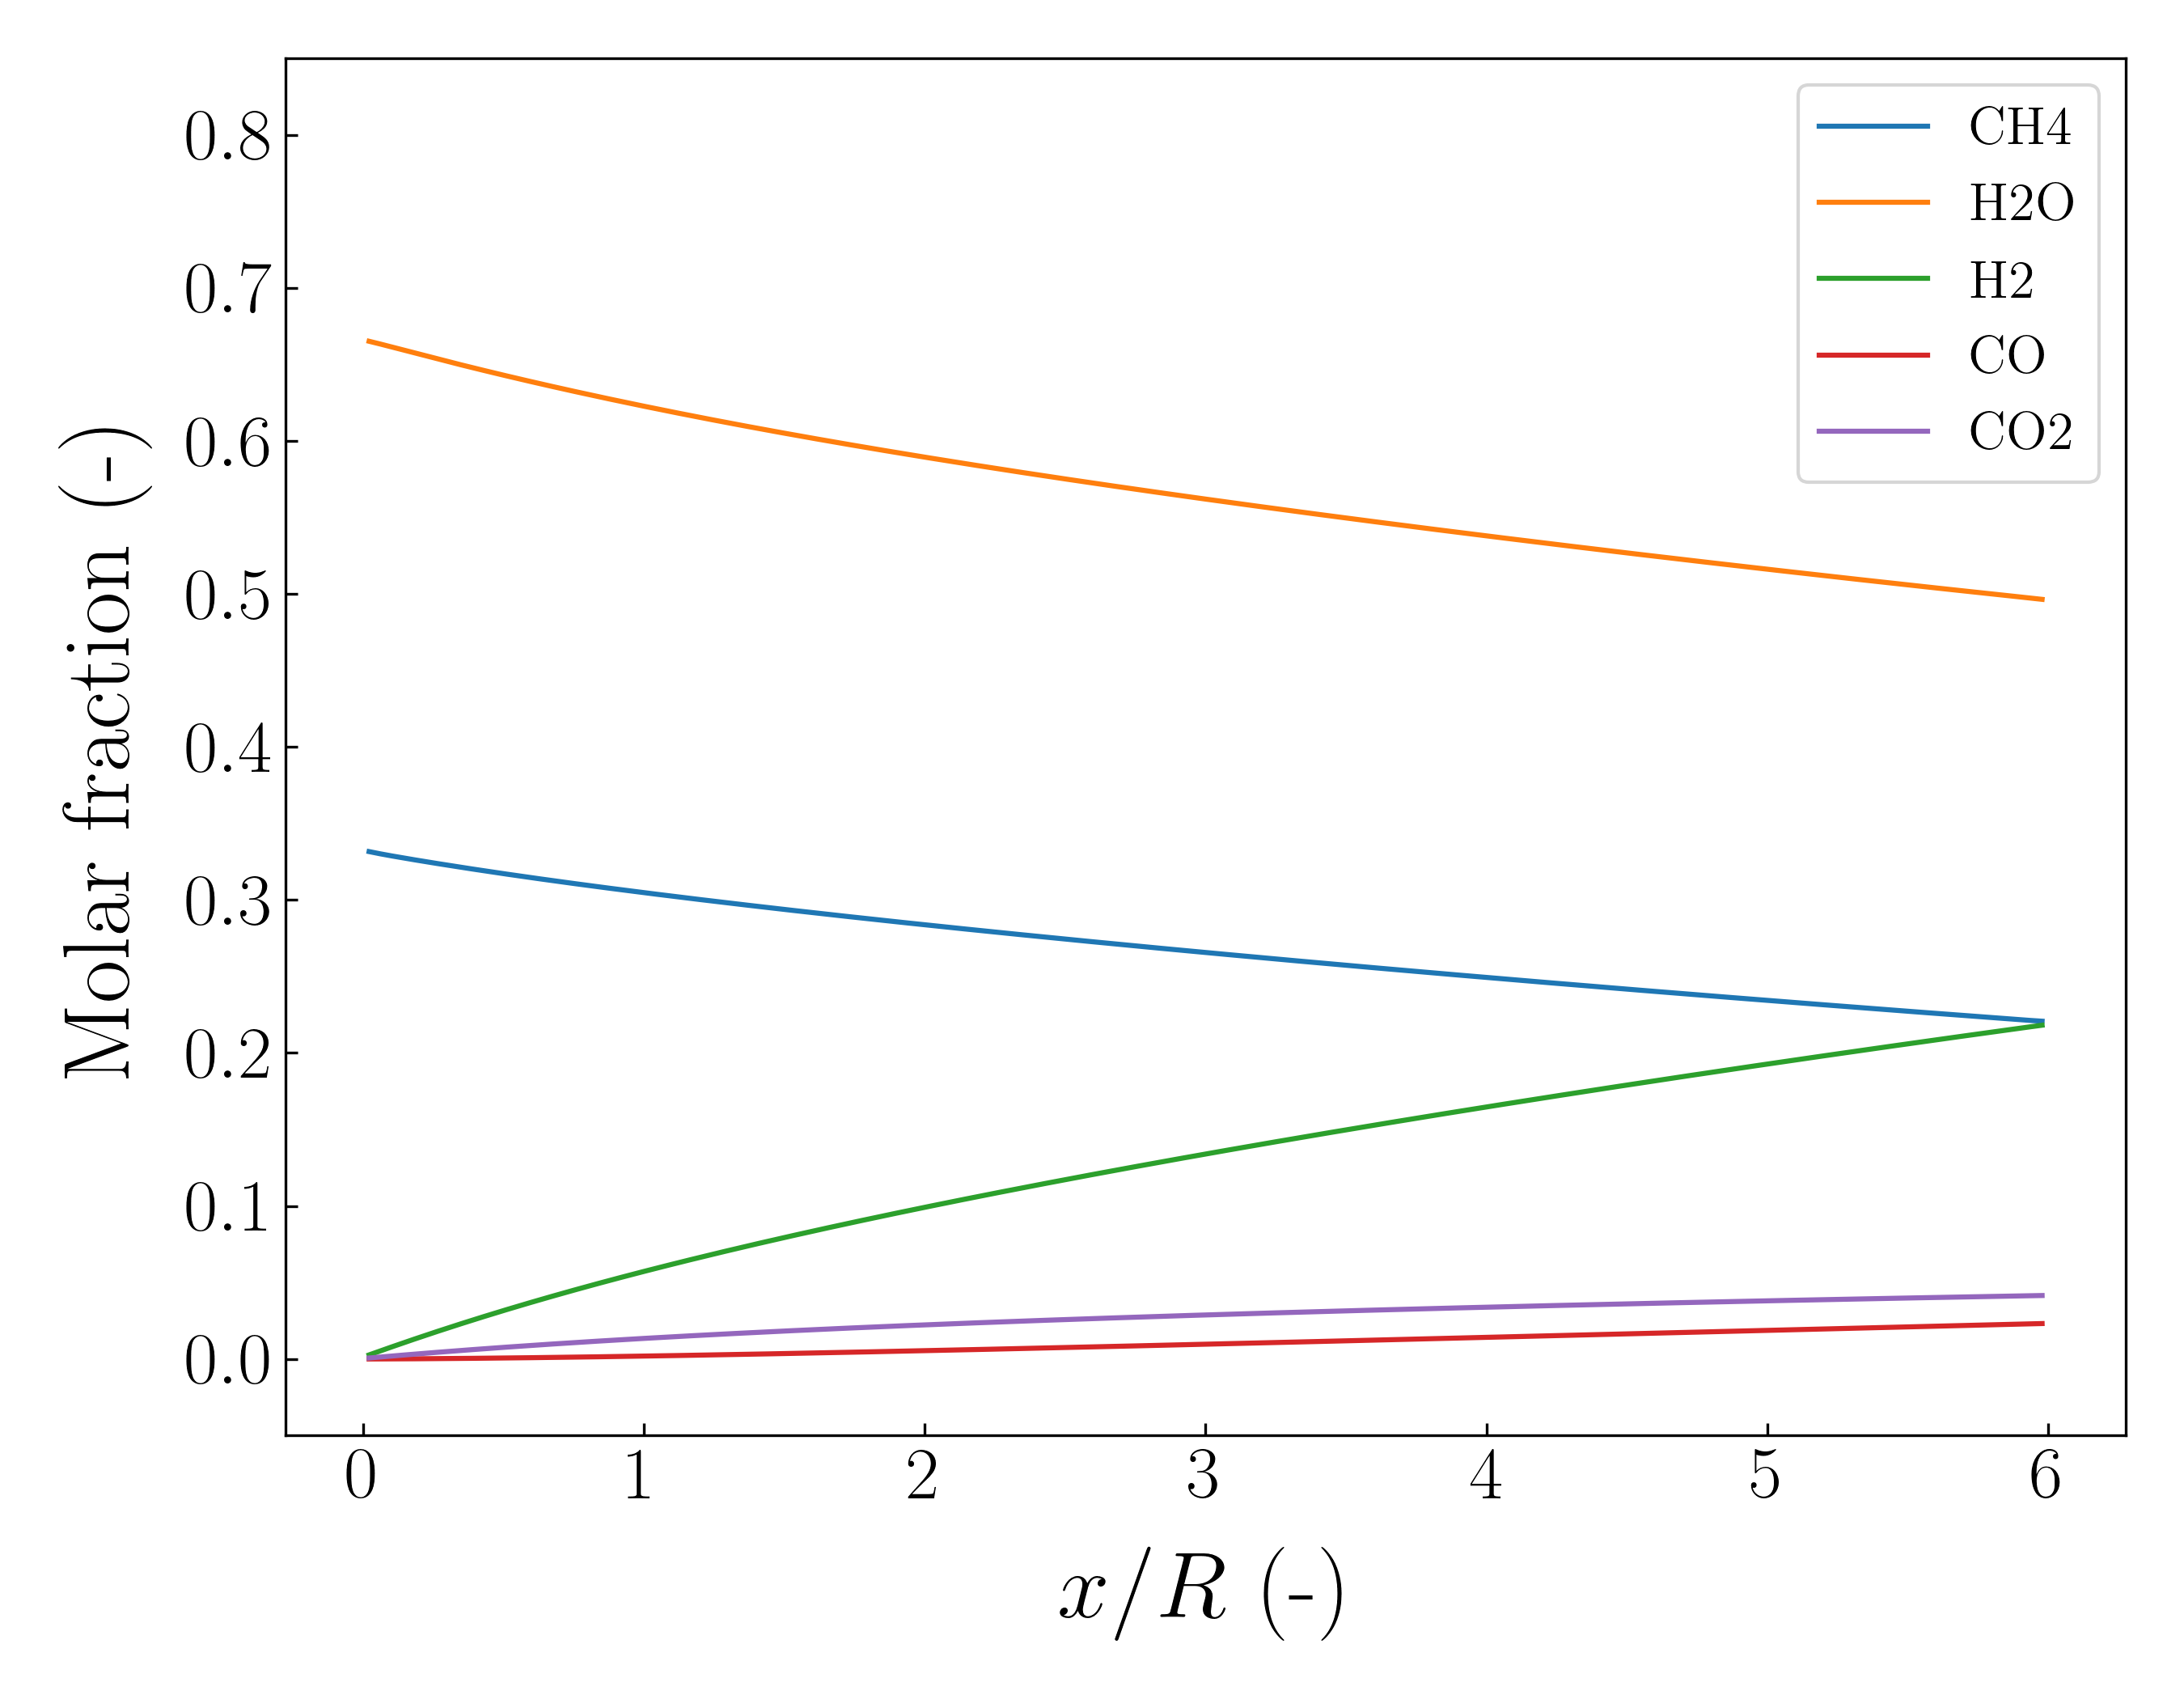
\includegraphics[width=80mm]{results/5/80C_20T/GEN30-AVG.png}
%\caption{\label{fig:5R8020G30-avg} Strategy I - Radius-averaged molar fractions -  30$^{\rm{th}}$ generation ($w_{\rm{CH_4}} = 0.8, w_T = 0.2$, $T_{\rm{in}}$ = 900 K, $u_{\rm{in}}$ = 0.15 m s$^{-1}$, $SC$ = 2.0)}
%\end{figure}
%
%
%The development of the fitness values among successive populations for strategy I is presented in Fig. \ref{fig:5R8020G-fitness}. 
%
%\begin{figure}
%\centering
%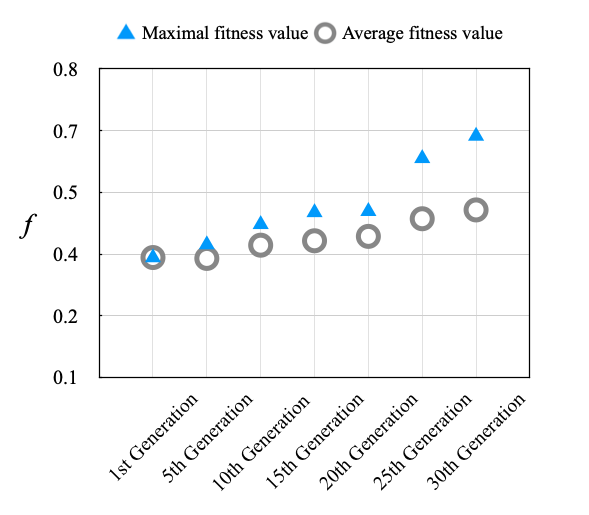
\includegraphics[width=100mm]{results/5/80C_20T.png}
%\caption{\label{fig:5R8020G-fitness} Strategy I - Fitness analysis throughout successive populations ($w_{\rm{CH_4}} = 0.8, w_T = 0.2$, $T_{\rm{in}}$ = 900 K, $u_{\rm{in}}$ = 0.15 m s$^{-1}$, $SC$ = 2.0)}
%\end{figure}
%
%To allow a straightforward comparison between the catalyst inserts division strategies, hydrogen productivity $\zeta$ is calculated for the optimal cases found by each algorithm. The hydrogen productivity is summarized in Table \ref{tab:5RH2prod}. 
%
%\begin{center}
%\begin{table}
%\centering
%\caption{Hydrogen productivity for the catalytic insert division strategy I}
%\label{tab:5RH2prod}
%\begin{tabular}{l|c|c|c}
%\hline\noalign{\smallskip}
% $w_{\rm{CH_4}}$ / $ w_T $ & $\rm{H_{2_{out}}}$ & $\iota$ & $\zeta$ \\
%\noalign{\smallskip}\hline\noalign{\smallskip}
%REF         & 0.581     & 1.00  &  0.581\\
%0.2 / 0.8   & 0.255     & 0.20  & 1.278 \\
%0.4 / 0.6   & 0.268     & 0.19  & 1.398 \\
%0.5 / 0.5   & 0.231     & 0.20  & 1.157 \\
%0.6 / 0.4   & 0.407     & 0.45  & 0.900 \\
%0.8 / 0.2   & 0.218     & 0.20  & 1.090 \\
%\noalign{\smallskip}\hline
%\end{tabular}
%\end{table}
%\end{center}
%
%
%\clearpage
%
%
%\subsection{Insert division strategy II}
%\label{subsec:5RE}
%
%\begin{figure}[h!]
%\centering
%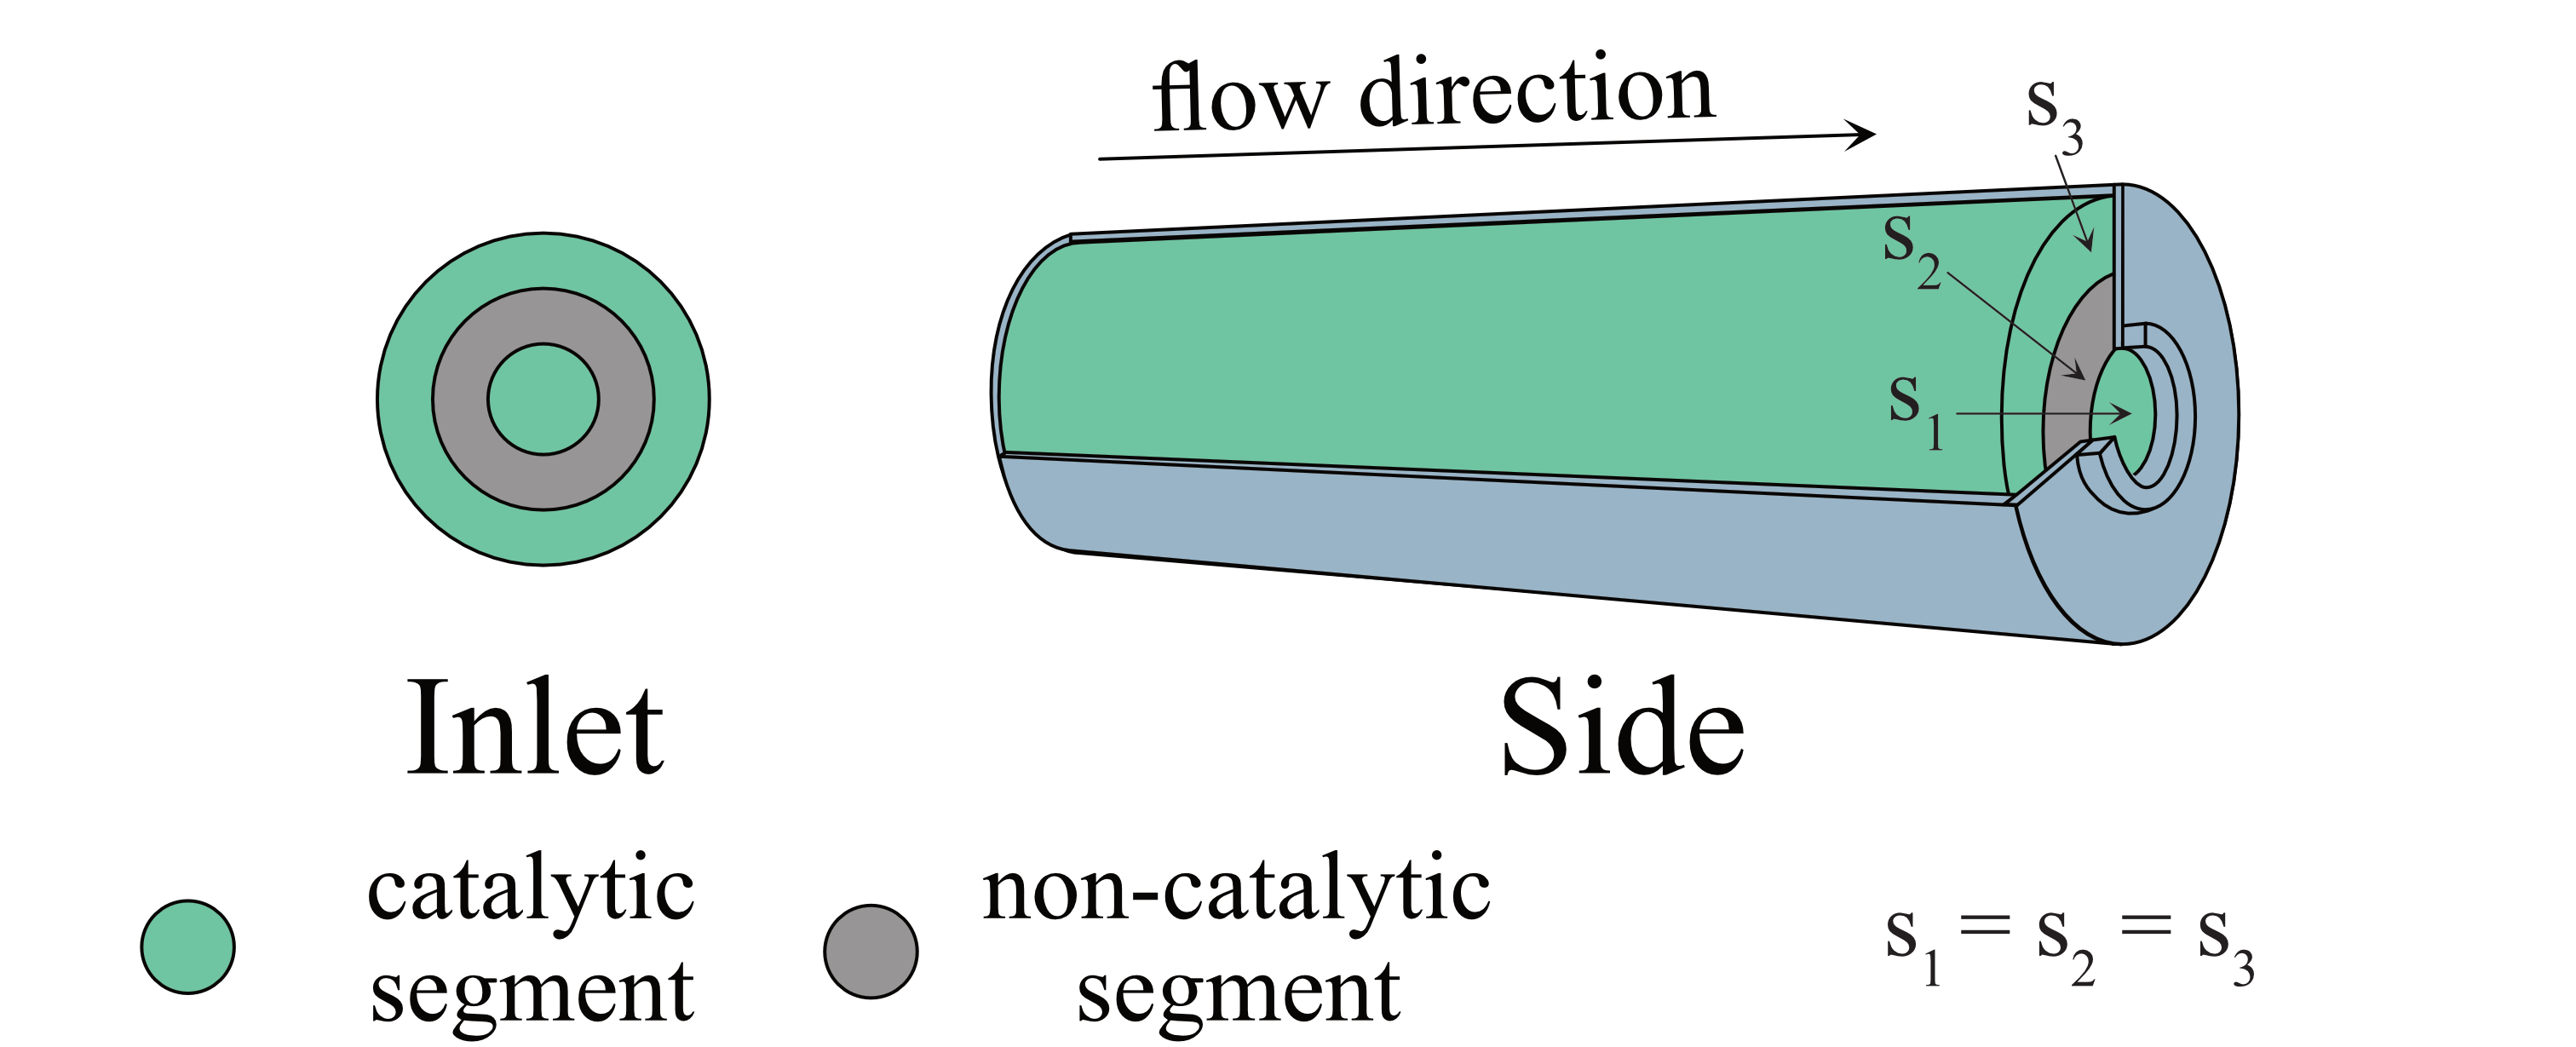
\includegraphics[width=120mm]{5segEqSurf.png}
%\caption{\label{fig:5segEqSurf}Catalytic insert division strategy II}
%\end{figure}
%
%
%\paragraph{Thermal fitness 80 \%, methane conversion 20 \%} \hspace{0pt} \\
%\noindent 
%
%
%\begin{figure}[h!]
%\centering
%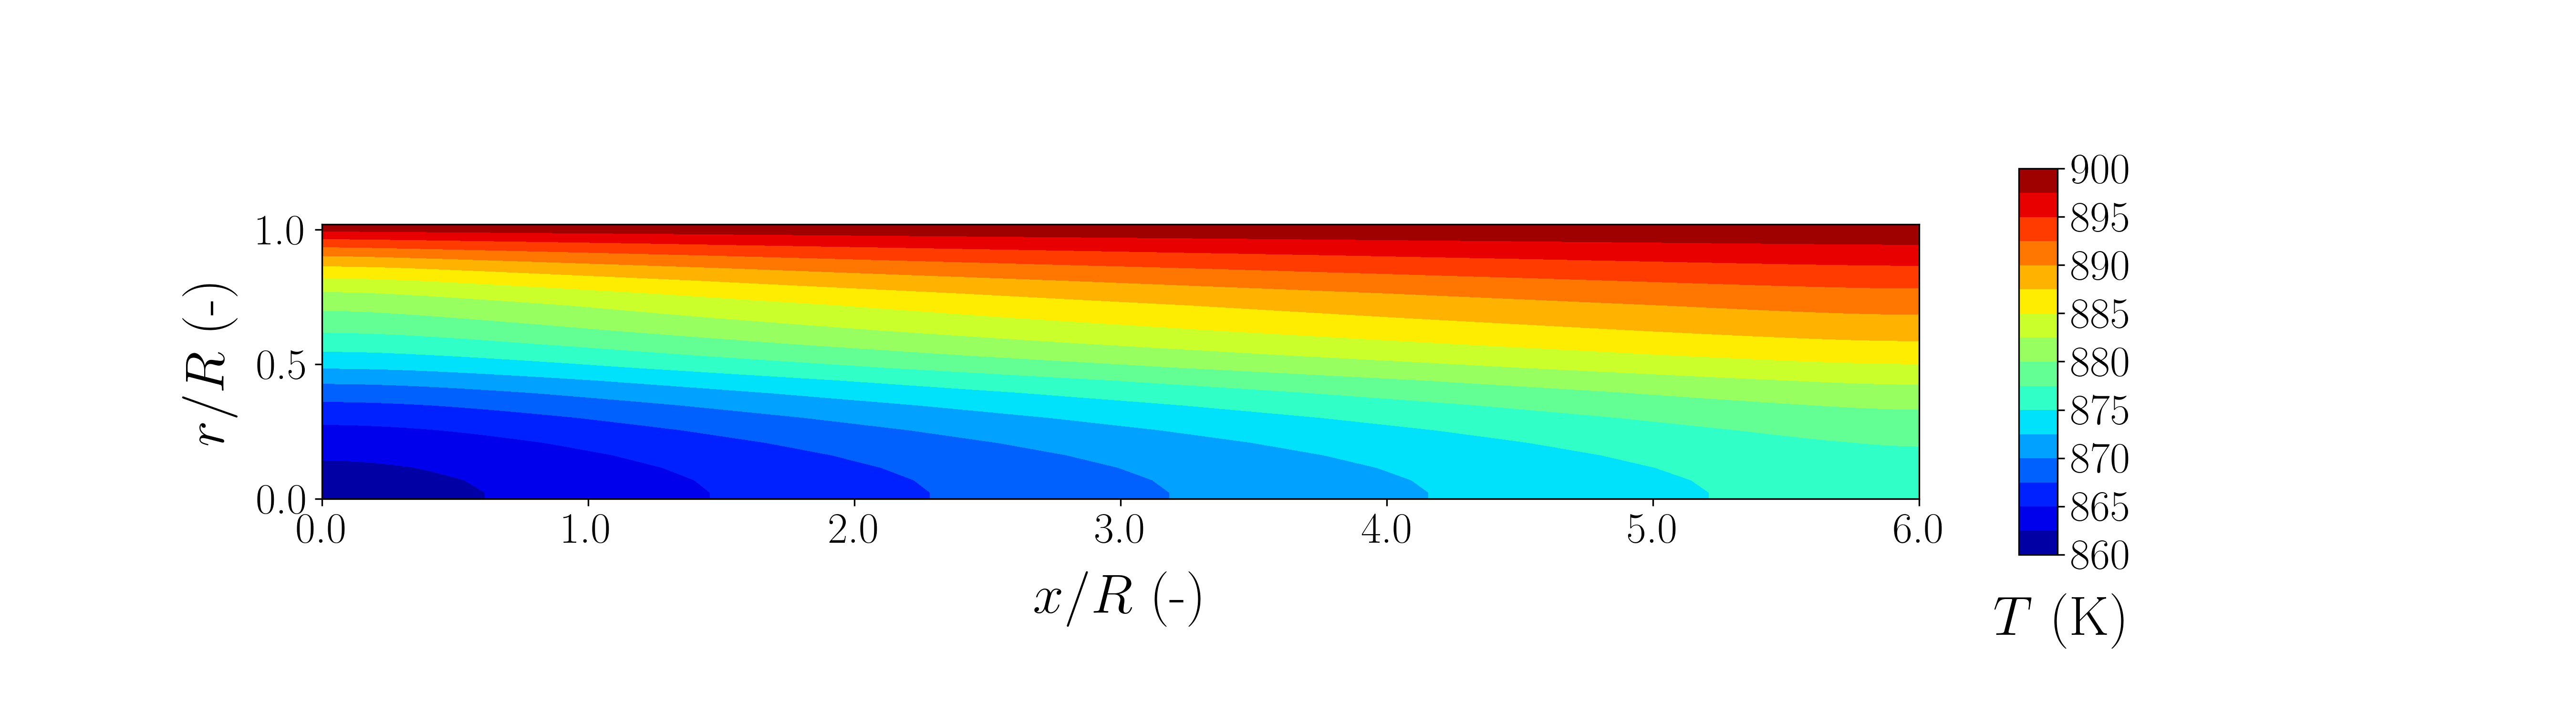
\includegraphics[width=190mm]{results/5Eq/20C_80T/GEN1-TFIELD.png}
%\caption{\label{fig:5RES2080G1-TField} Strategy II - Temperature field distribution - 1$^{\rm{st}}$ generation ($w_{\rm{CH_4}} = 0.2, w_T = 0.8$, $T_{\rm{in}}$ = 900 K, $u_{\rm{in}}$ = 0.15 m s$^{-1}$, $SC$ = 2.0)}
%\end{figure}
%
%\begin{figure}[h!]
%\centering
%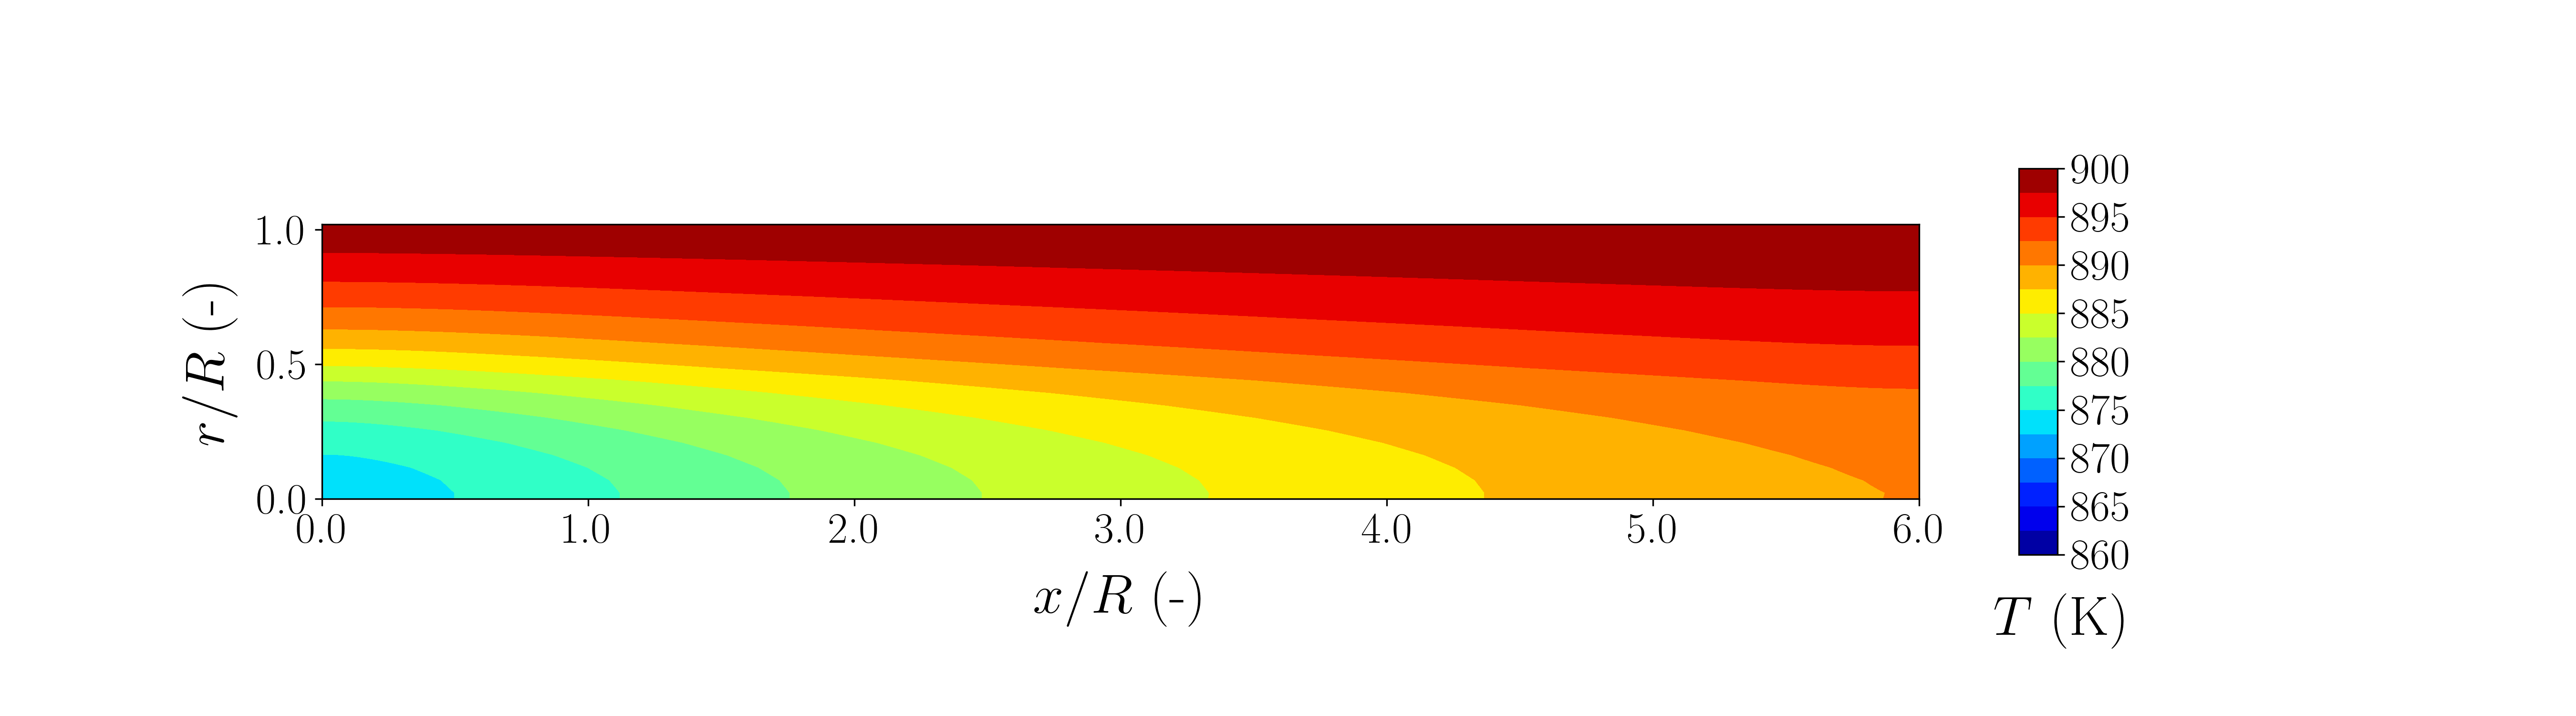
\includegraphics[width=190mm]{results/5Eq/20C_80T/GEN15-TFIELD.png}
%\caption{\label{fig:5RES2080G15-TField} Strategy II - Temperature field distribution - 15$^{\rm{th}}$ generation ($w_{\rm{CH_4}} = 0.2, w_T = 0.8$, $T_{\rm{in}}$ = 900 K, $u_{\rm{in}}$ = 0.15 m s$^{-1}$, $SC$ = 2.0)}
%\end{figure}
%
%\begin{figure}[h!]
%\centering
%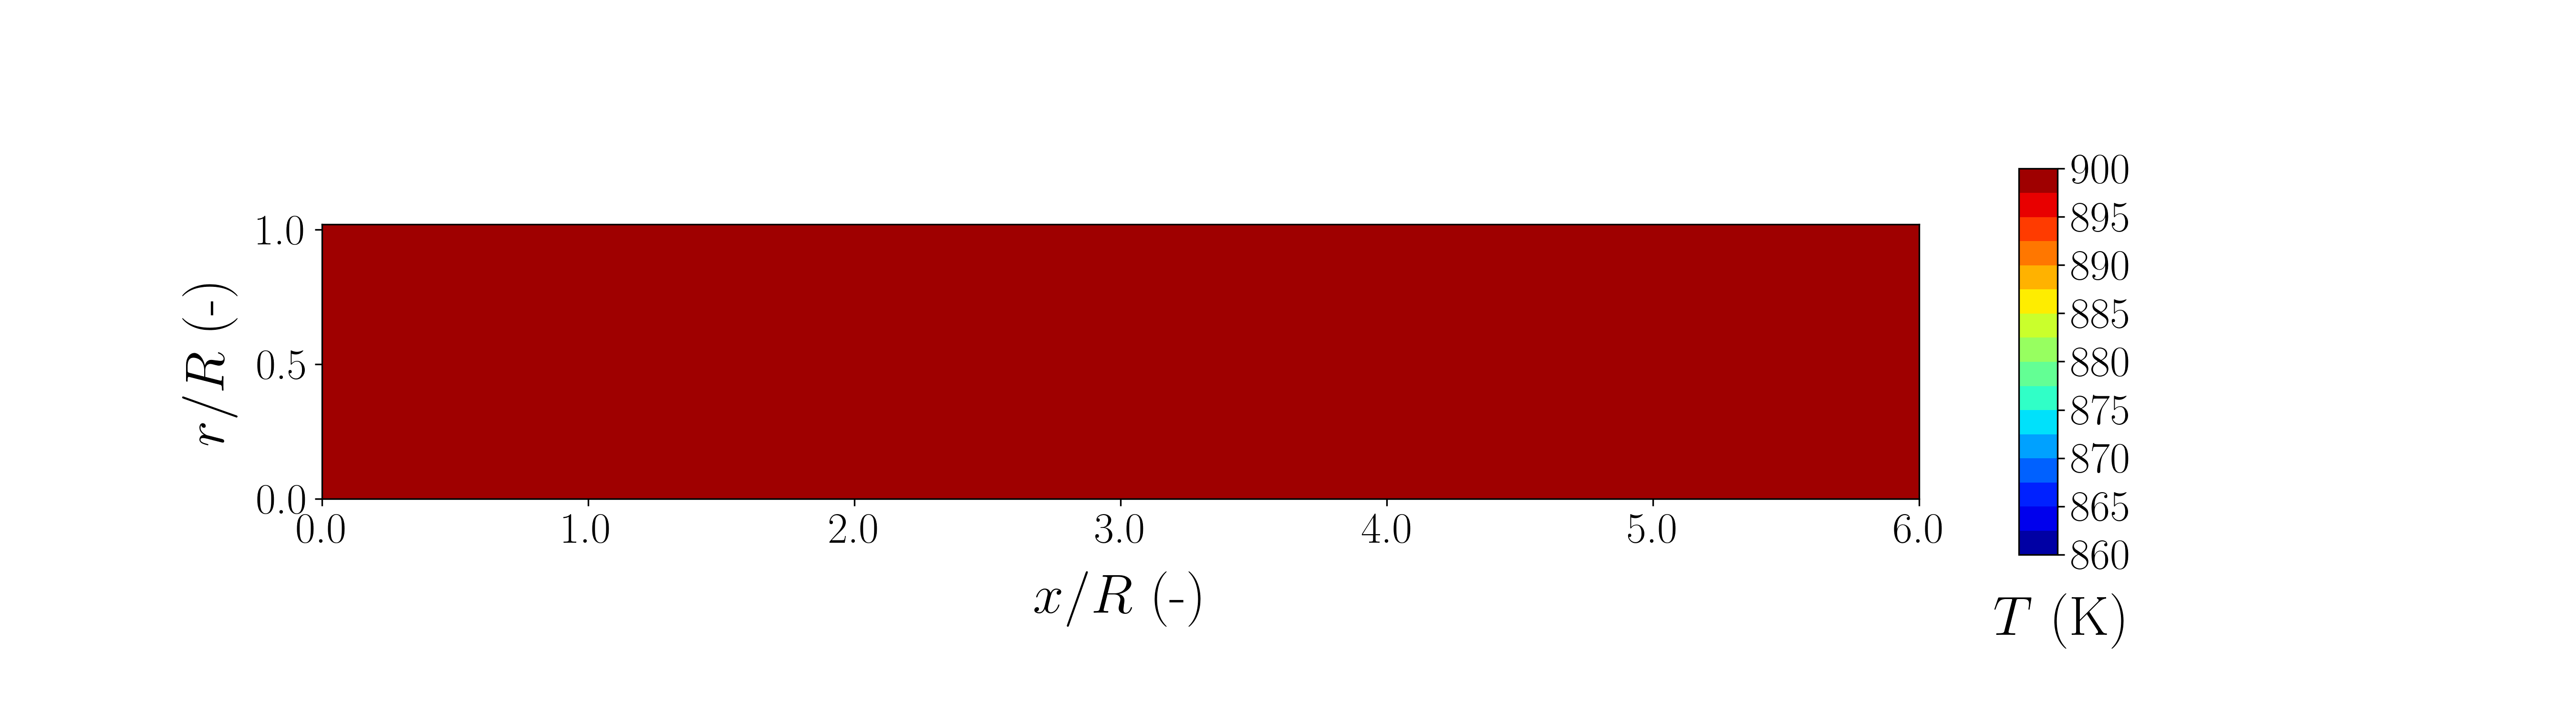
\includegraphics[width=190mm]{results/5Eq/20C_80T/GEN30-TFIELD.png}
%\caption{\label{fig:5RES2080G30-TField} Strategy II - Temperature field distribution - 30$^{\rm{th}}$ generation ($w_{\rm{CH_4}} = 0.2, w_T = 0.8$, $T_{\rm{in}}$ = 900 K, $u_{\rm{in}}$ = 0.15 m s$^{-1}$, $SC$ = 2.0)}
%\end{figure}
%
%
%\begin{figure}[h!]
%\centering
%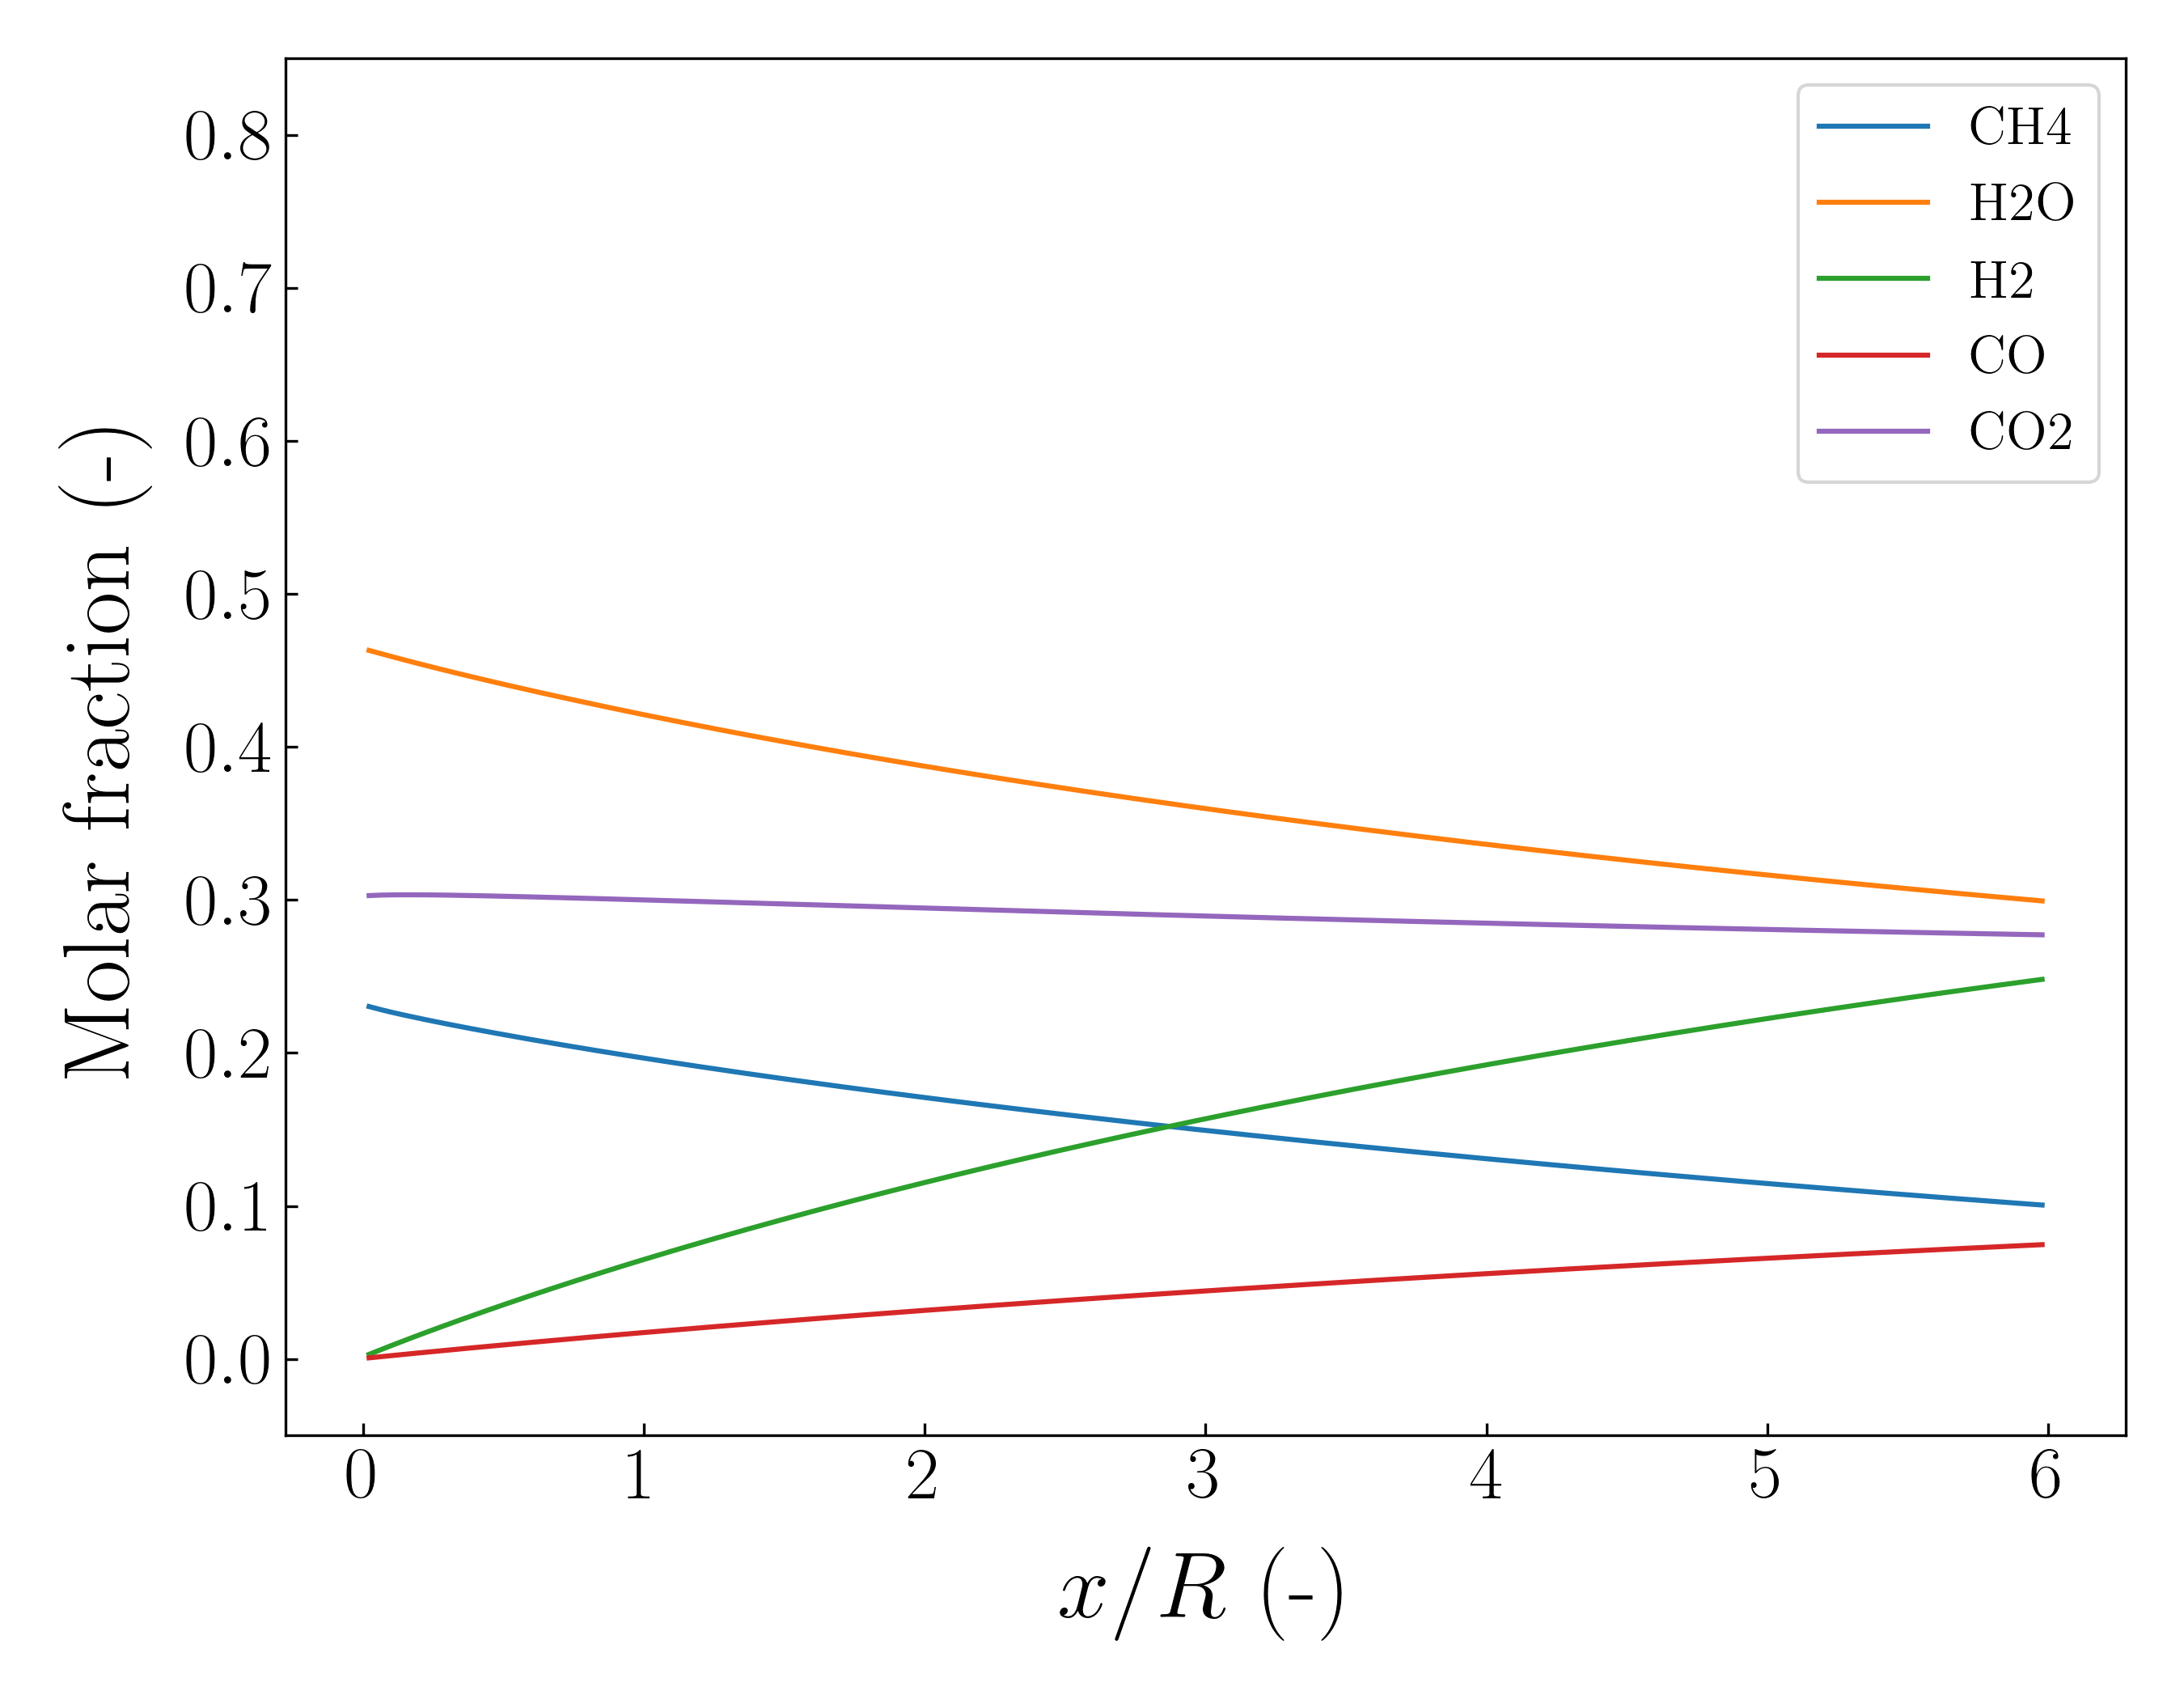
\includegraphics[width=80mm]{results/5Eq/20C_80T/GEN1-AVG.png}
%\caption{\label{fig:5RES2080G1-avg} Strategy II - Radius-averaged molar fractions - 1$^{\rm{st}}$ generation ($w_{\rm{CH_4}} = 0.2, w_T = 0.8$, $T_{\rm{in}}$ = 900 K, $u_{\rm{in}}$ = 0.15 m s$^{-1}$, $SC$ = 2.0)}
%\end{figure}
%
%\begin{figure}[h!]
%\centering
%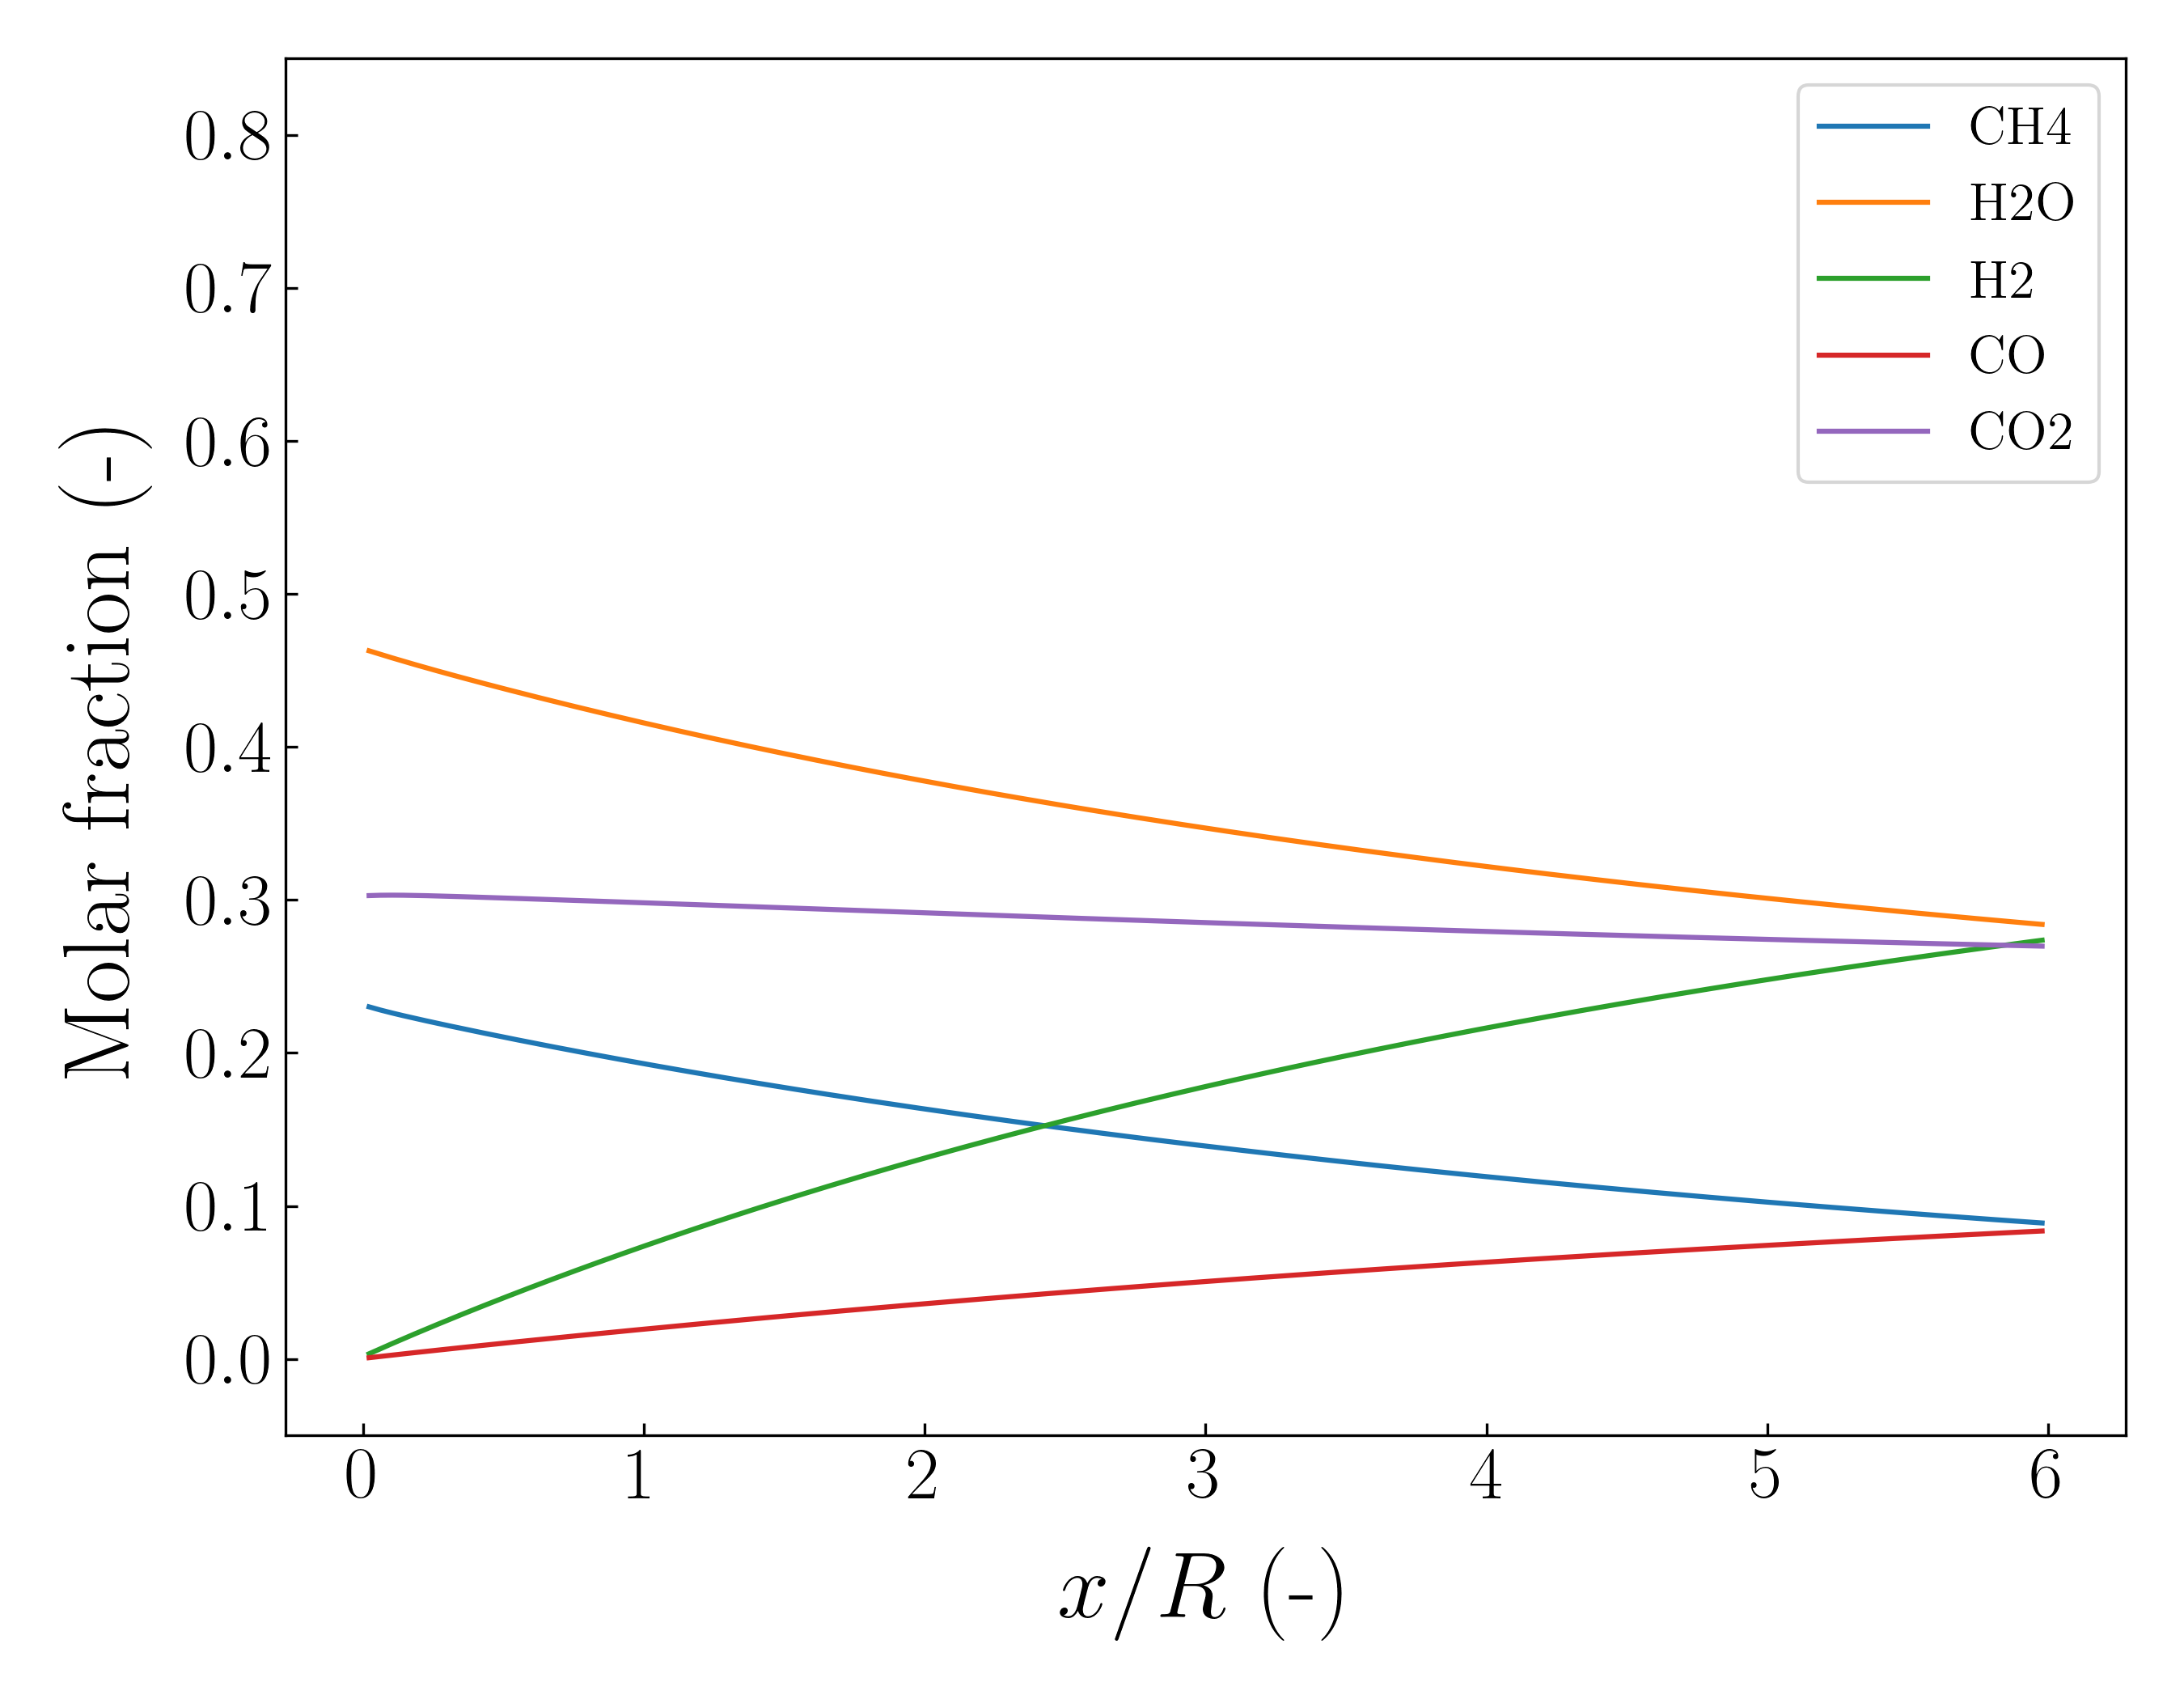
\includegraphics[width=80mm]{results/5Eq/20C_80T/GEN15-AVG.png}
%\caption{\label{fig:5RES2080G15-avg} Strategy II - Radius-averaged molar fractions - 15$^{\rm{th}}$ generation ($w_{\rm{CH_4}} = 0.2, w_T = 0.8$, $T_{\rm{in}}$ = 900 K, $u_{\rm{in}}$ = 0.15 m s$^{-1}$, $SC$ = 2.0)}
%\end{figure}
%
%\begin{figure}[h!]
%\centering
%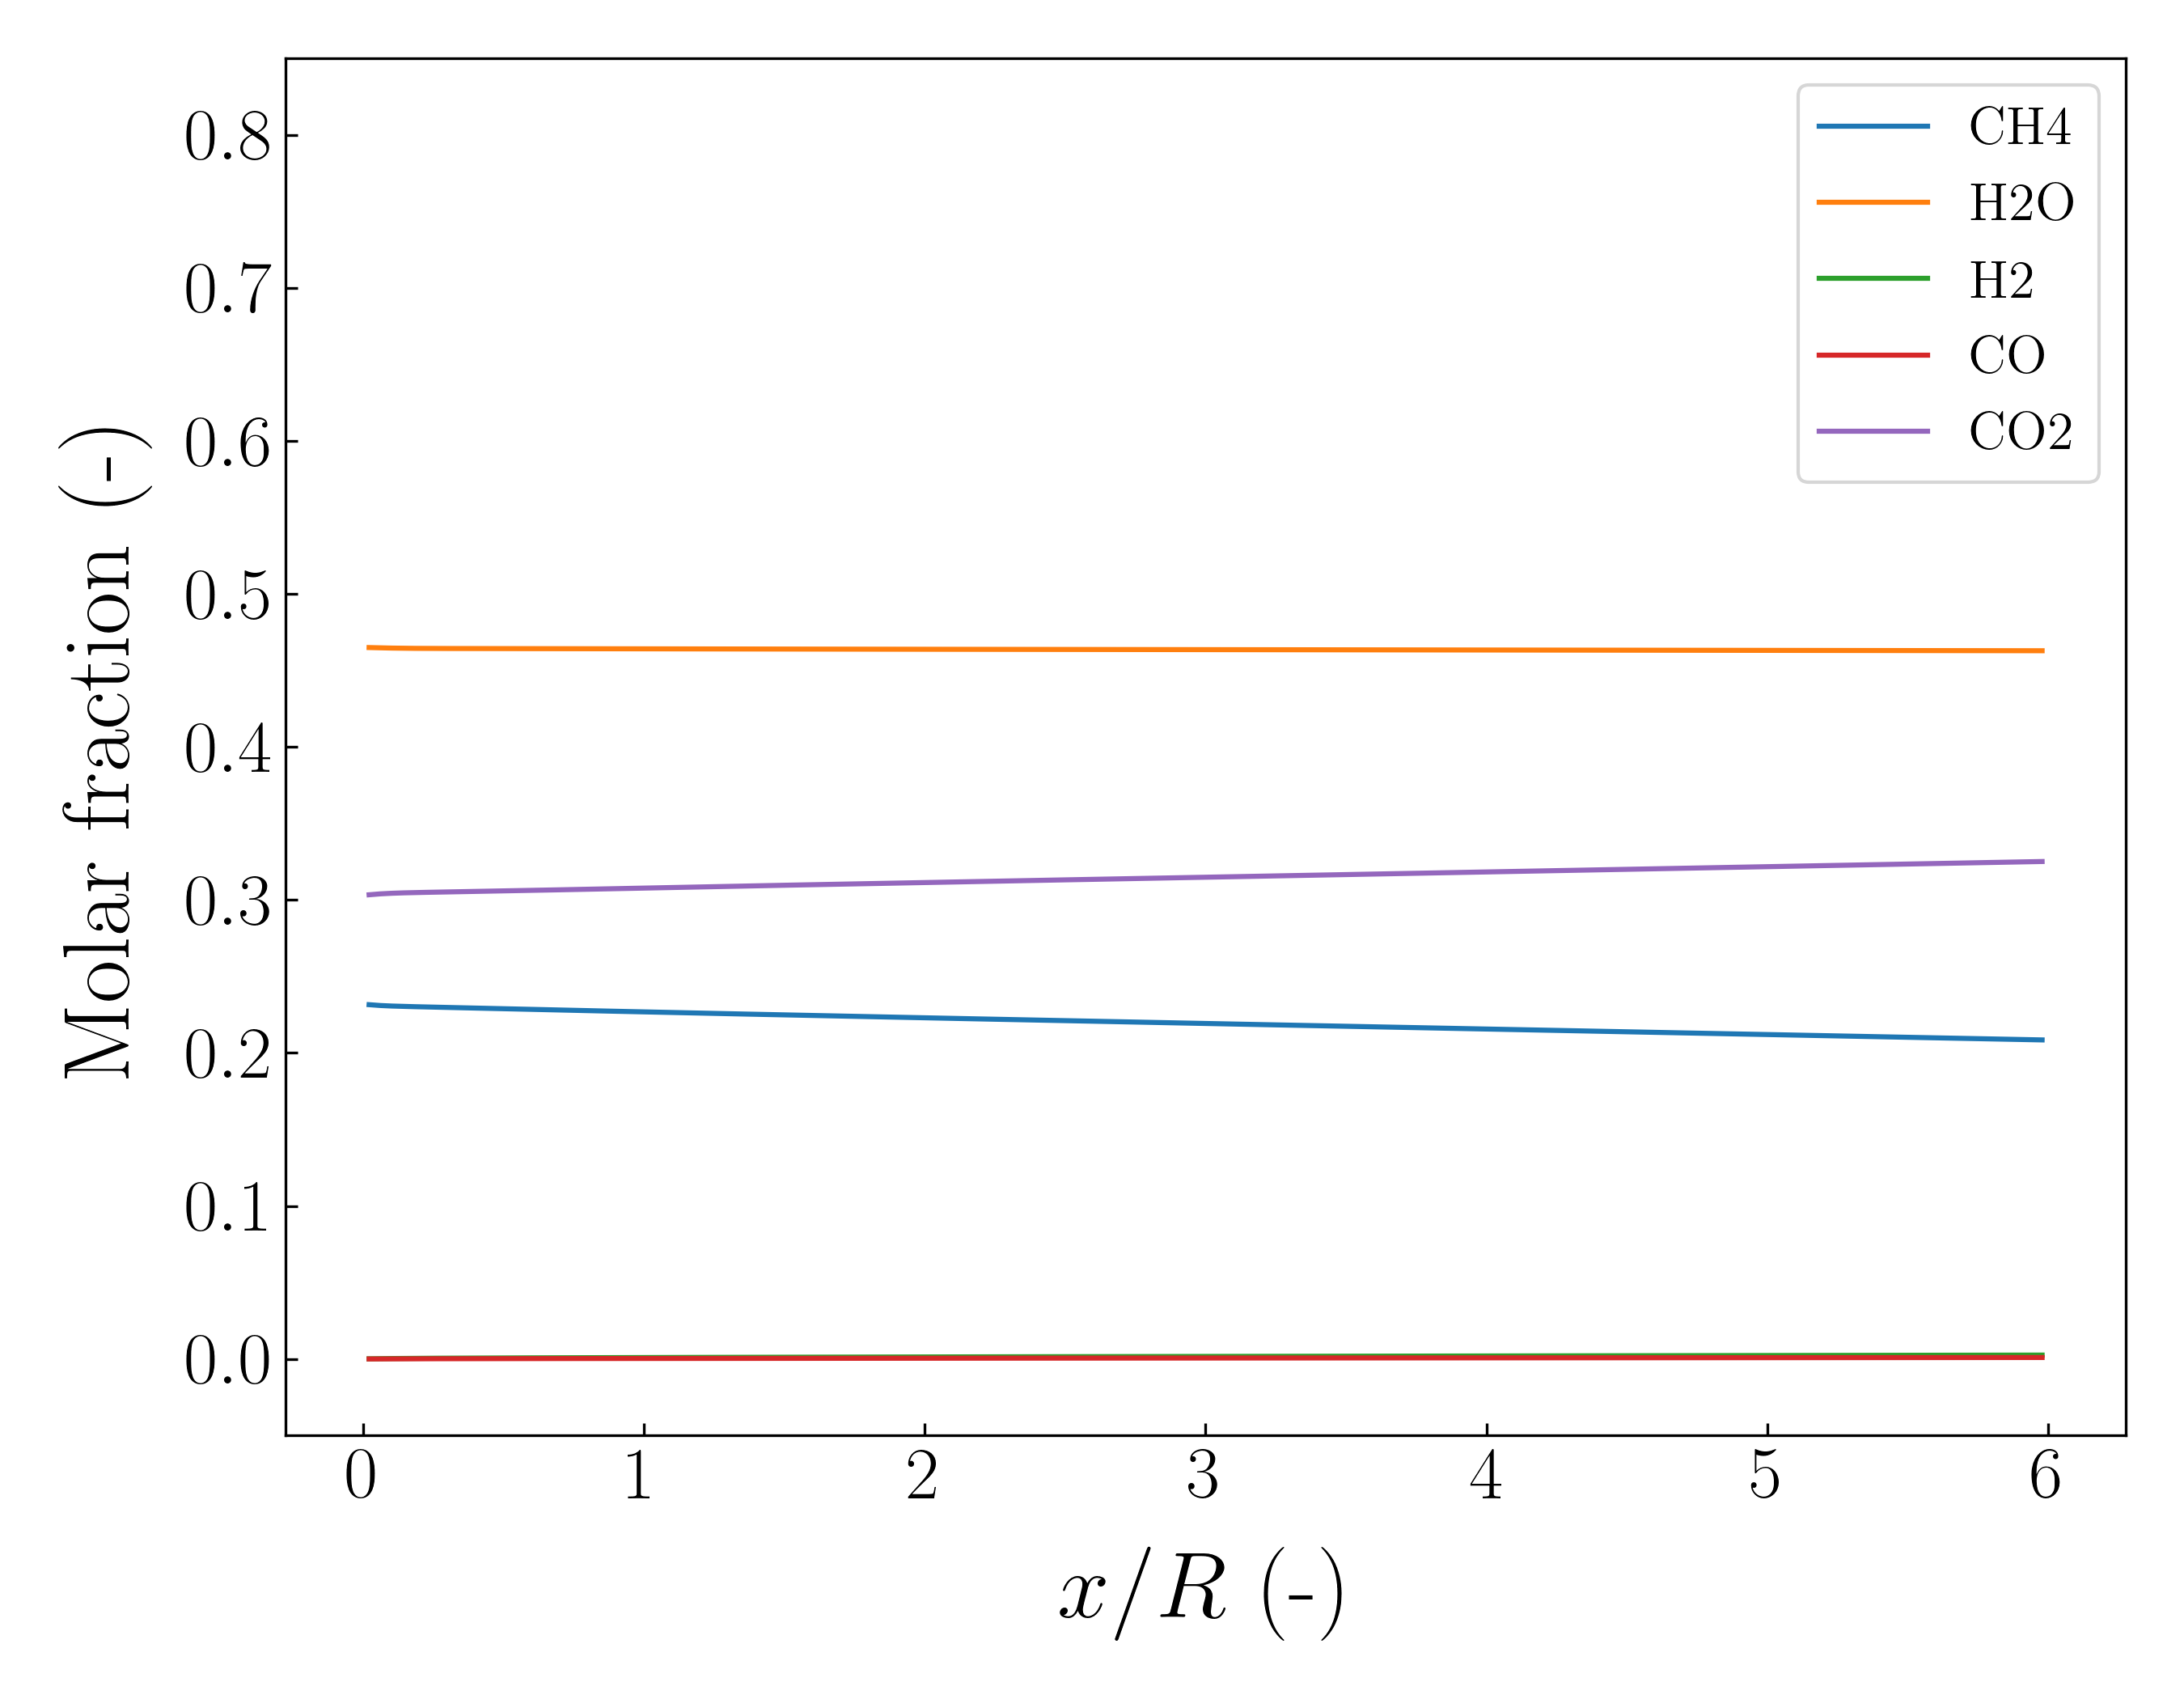
\includegraphics[width=80mm]{results/5Eq/20C_80T/GEN30-AVG.png}
%\caption{\label{fig:5RES2080G30-avg} Strategy II - Radius-averaged molar fractions -  30$^{\rm{th}}$ generation ($w_{\rm{CH_4}} = 0.2, w_T = 0.8$, $T_{\rm{in}}$ = 900 K, $u_{\rm{in}}$ = 0.15 m s$^{-1}$, $SC$ = 2.0)}
%\end{figure}
%
%\begin{figure}[h!]
%\centering
%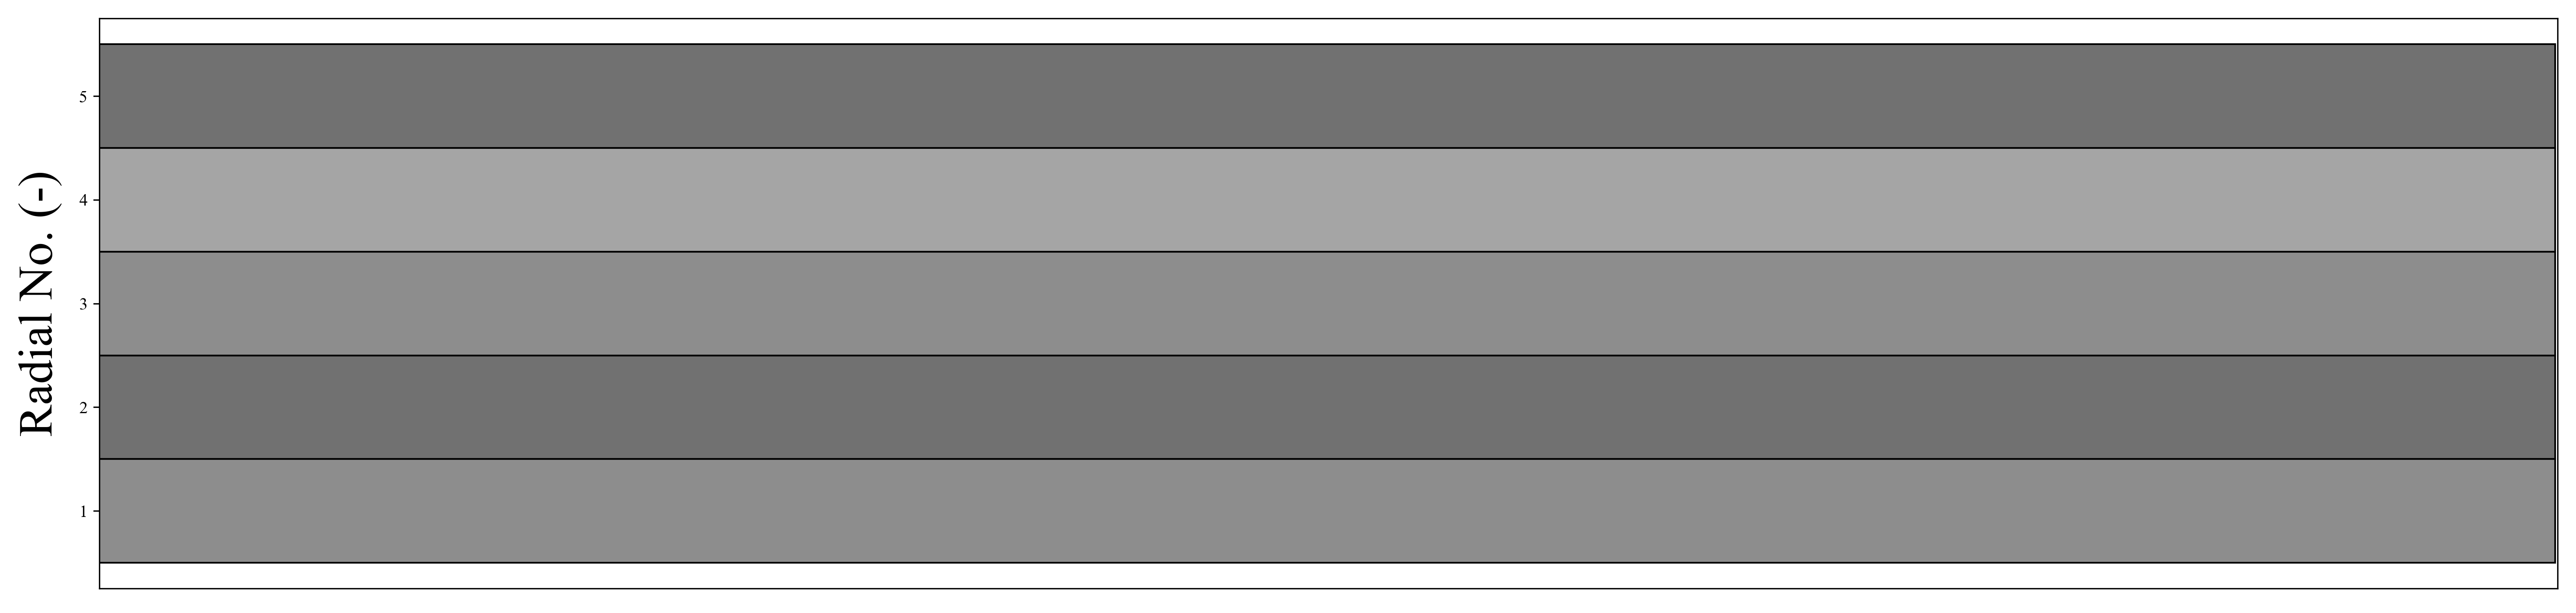
\includegraphics[width=120mm]{results/segments/5segEq/20C80T/seg.png}
%\caption{\label{fig:30L6040G1-TField} Strategy II - Segments distribution for 30$^{\rm{th}}$ generation ($w_{\rm{CH_4}} = 0.2, w_T = 0.8$, $T_{\rm{in}}$ = 900 K, $u_{\rm{in}}$ = 0.15 m s$^{-1}$, $SC$ = 2.0)}
%\end{figure}
%
%\begin{figure}[h!]
%\centering
%\includegraphics[width=100mm]{results/5Eq/20C_80T.png}
%\caption{\label{fig:5RES2080G-fitness} Strategy II - Fitness analysis throughout successive populations ($w_{\rm{CH_4}} = 0.2, w_T = 0.8$, $T_{\rm{in}}$ = 900 K, $u_{\rm{in}}$ = 0.15 m s$^{-1}$, $SC$ = 2.0)}
%\end{figure}
%
%
%
%\clearpage
%
%
%
%\paragraph{Thermal fitness 60 \%, methane conversion 40 \%} \hspace{0pt} \\
%\noindent 
%
%
%\begin{figure}[h!]
%\centering
%\includegraphics[width=190mm]{results/5Eq/40C_60T/GEN1-TFIELD.png}
%\caption{\label{fig:5RES4060G1-TField} Strategy II - Temperature field distribution - 1$^{\rm{st}}$ generation ($w_{\rm{CH_4}} = 0.4, w_T = 0.6$, $T_{\rm{in}}$ = 900 K, $u_{\rm{in}}$ = 0.15 m s$^{-1}$, $SC$ = 2.0)}
%\end{figure}
%
%\begin{figure}[h!]
%\centering
%\includegraphics[width=190mm]{results/5Eq/40C_60T/GEN15-TFIELD.png}
%\caption{\label{fig:5RES4060G15-TField} Strategy II - Temperature field distribution - 15$^{\rm{th}}$ generation ($w_{\rm{CH_4}} = 0.4, w_T = 0.6$, $T_{\rm{in}}$ = 900 K, $u_{\rm{in}}$ = 0.15 m s$^{-1}$, $SC$ = 2.0)}
%\end{figure}
%
%\begin{figure}[h!]
%\centering
%\includegraphics[width=190mm]{results/5Eq/40C_60T/GEN30-TFIELD.png}
%\caption{\label{fig:5RES4060G30-TField} Strategy II - Temperature field distribution - 30$^{\rm{th}}$ generation ($w_{\rm{CH_4}} = 0.4, w_T = 0.6$, $T_{\rm{in}}$ = 900 K, $u_{\rm{in}}$ = 0.15 m s$^{-1}$, $SC$ = 2.0)}
%\end{figure}
%
%
%\begin{figure}[h!]
%\centering
%\includegraphics[width=80mm]{results/5Eq/40C_60T/GEN1-AVG.png}
%\caption{\label{fig:5RES4060G1-avg} Strategy II - Radius-averaged molar fractions - 1$^{\rm{st}}$ generation ($w_{\rm{CH_4}} = 0.4, w_T = 0.6$, $T_{\rm{in}}$ = 900 K, $u_{\rm{in}}$ = 0.15 m s$^{-1}$, $SC$ = 2.0)}
%\end{figure}
%
%\begin{figure}[h!]
%\centering
%\includegraphics[width=80mm]{results/5Eq/40C_60T/GEN15-AVG.png}
%\caption{\label{fig:5RES4060G15-avg} Strategy II - Radius-averaged molar fractions - 15$^{\rm{th}}$ generation ($w_{\rm{CH_4}} = 0.4, w_T = 0.6$, $T_{\rm{in}}$ = 900 K, $u_{\rm{in}}$ = 0.15 m s$^{-1}$, $SC$ = 2.0)}
%\end{figure}
%
%\begin{figure}[h!]
%\centering
%\includegraphics[width=80mm]{results/5Eq/40C_60T/GEN30-AVG.png}
%\caption{\label{fig:5RES4060G30-avg} Strategy II - Radius-averaged molar fractions -  30$^{\rm{th}}$ generation ($w_{\rm{CH_4}} = 0.4, w_T = 0.6$, $T_{\rm{in}}$ = 900 K, $u_{\rm{in}}$ = 0.15 m s$^{-1}$, $SC$ = 2.0)}
%\end{figure}
%
%\begin{figure}[h!]
%\centering
%\includegraphics[width=120mm]{results/segments/5segEq/40C60T/seg.png}
%\caption{\label{fig:30L6040G1-TField} Strategy II - Segments distribution for 30$^{\rm{th}}$ generation ($w_{\rm{CH_4}} = 0.4, w_T = 0.6$, $T_{\rm{in}}$ = 900 K, $u_{\rm{in}}$ = 0.15 m s$^{-1}$, $SC$ = 2.0)}
%\end{figure}
%
%\begin{figure}[h!]
%\centering
%\includegraphics[width=100mm]{results/5Eq/40C_60T.png}
%\caption{\label{fig:5RES4060G-fitness} Strategy II - Fitness analysis throughout successive populations ($w_{\rm{CH_4}} = 0.4, w_T = 0.6$, $T_{\rm{in}}$ = 900 K, $u_{\rm{in}}$ = 0.15 m s$^{-1}$, $SC$ = 2.0)}
%\end{figure}
%
%
%\clearpage
%
%
%
%
%
%\paragraph{Thermal fitness 50 \%, methane conversion 50 \%} \hspace{0pt} \\
%\noindent 
%
%
%\begin{figure}[h!]
%\centering
%\includegraphics[width=190mm]{results/5Eq/50C_50T/GEN1-TFIELD.png}
%\caption{\label{fig:5RES5050G1-TField} Strategy II - Temperature field distribution - 1$^{\rm{st}}$ generation ($w_{\rm{CH_4}} = 0.5, w_T = 0.5$, $T_{\rm{in}}$ = 900 K, $u_{\rm{in}}$ = 0.15 m s$^{-1}$, $SC$ = 2.0)}
%\end{figure}
%
%\begin{figure}[h!]
%\centering
%\includegraphics[width=190mm]{results/5Eq/50C_50T/GEN15-TFIELD.png}
%\caption{\label{fig:5RES5050G15-TField} Strategy II - Temperature field distribution - 15$^{\rm{th}}$ generation ($w_{\rm{CH_4}} = 0.5, w_T = 0.5$, $T_{\rm{in}}$ = 900 K, $u_{\rm{in}}$ = 0.15 m s$^{-1}$, $SC$ = 2.0)}
%\end{figure}
%
%\begin{figure}[h!]
%\centering
%\includegraphics[width=190mm]{results/5Eq/50C_50T/GEN30-TFIELD.png}
%\caption{\label{fig:5RES5050G30-TField} Strategy II - Temperature field distribution - 30$^{\rm{th}}$ generation ($w_{\rm{CH_4}} = 0.5, w_T = 0.5$, $T_{\rm{in}}$ = 900 K, $u_{\rm{in}}$ = 0.15 m s$^{-1}$, $SC$ = 2.0)}
%\end{figure}
%
%
%\begin{figure}[h!]
%\centering
%\includegraphics[width=80mm]{results/5Eq/50C_50T/GEN1-AVG.png}
%\caption{\label{fig:5RES5050G1-avg} Strategy II - Radius-averaged molar fractions - 1$^{\rm{st}}$ generation ($w_{\rm{CH_4}} = 0.5, w_T = 0.5$, $T_{\rm{in}}$ = 900 K, $u_{\rm{in}}$ = 0.15 m s$^{-1}$, $SC$ = 2.0)}
%\end{figure}
%
%\begin{figure}[h!]
%\centering
%\includegraphics[width=80mm]{results/5Eq/50C_50T/GEN15-AVG.png}
%\caption{\label{fig:5RES5050G15-avg} Strategy II - Radius-averaged molar fractions - 15$^{\rm{th}}$ generation ($w_{\rm{CH_4}} = 0.5, w_T = 0.5$, $T_{\rm{in}}$ = 900 K, $u_{\rm{in}}$ = 0.15 m s$^{-1}$, $SC$ = 2.0)}
%\end{figure}
%
%\begin{figure}[h!]
%\centering
%\includegraphics[width=80mm]{results/5Eq/50C_50T/GEN30-AVG.png}
%\caption{\label{fig:5RES5050G30-avg} Strategy II - Radius-averaged molar fractions -  30$^{\rm{th}}$ generation ($w_{\rm{CH_4}} = 0.5, w_T = 0.5$, $T_{\rm{in}}$ = 900 K, $u_{\rm{in}}$ = 0.15 m s$^{-1}$, $SC$ = 2.0)}
%\end{figure}
%
%\begin{figure}[h!]
%\centering
%\includegraphics[width=120mm]{results/segments/5segEq/50C50T/seg.png}
%\caption{\label{fig:30L6040G1-TField} Strategy II - Segments distribution for 30$^{\rm{th}}$ generation ($w_{\rm{CH_4}} = 0.5, w_T = 0.5$, $T_{\rm{in}}$ = 900 K, $u_{\rm{in}}$ = 0.15 m s$^{-1}$, $SC$ = 2.0)}
%\end{figure}
%
%
%\begin{figure}[h!]
%\centering
%\includegraphics[width=100mm]{results/5Eq/50C_50T.png}
%\caption{\label{fig:5RES5050G-fitness} Strategy II - Fitness analysis throughout successive populations ($w_{\rm{CH_4}} = 0.5, w_T = 0.5$, $T_{\rm{in}}$ = 900 K, $u_{\rm{in}}$ = 0.15 m s$^{-1}$, $SC$ = 2.0)}
%\end{figure}
%
%
%\clearpage
%
%
%
%\paragraph{Thermal fitness 40 \%, methane conversion 60 \%} \hspace{0pt} \\
%\noindent 
%
%
%\begin{figure}[h!]
%\centering
%\includegraphics[width=190mm]{results/5Eq/60C_40T/GEN1-TFIELD.png}
%\caption{\label{fig:5RES6040G1-TField} Strategy II - Temperature field distribution - 1$^{\rm{st}}$ generation ($w_{\rm{CH_4}} = 0.6, w_T = 0.4$, $T_{\rm{in}}$ = 900 K, $u_{\rm{in}}$ = 0.15 m s$^{-1}$, $SC$ = 2.0)}
%\end{figure}
%
%\begin{figure}[h!]
%\centering
%\includegraphics[width=190mm]{results/5Eq/60C_40T/GEN15-TFIELD.png}
%\caption{\label{fig:5RES6040G15-TField} Strategy II - Temperature field distribution - 15$^{\rm{th}}$ generation ($w_{\rm{CH_4}} = 0.6, w_T = 0.4$, $T_{\rm{in}}$ = 900 K, $u_{\rm{in}}$ = 0.15 m s$^{-1}$, $SC$ = 2.0)}
%\end{figure}
%
%\begin{figure}[h!]
%\centering
%\includegraphics[width=190mm]{results/5Eq/60C_40T/GEN30-TFIELD.png}
%\caption{\label{fig:5RES6040G30-TField} Strategy II - Temperature field distribution - 30$^{\rm{th}}$ generation ($w_{\rm{CH_4}} = 0.6, w_T = 0.4$, $T_{\rm{in}}$ = 900 K, $u_{\rm{in}}$ = 0.15 m s$^{-1}$, $SC$ = 2.0)}
%\end{figure}
%
%
%\begin{figure}[h!]
%\centering
%\includegraphics[width=80mm]{results/5Eq/60C_40T/GEN1-AVG.png}
%\caption{\label{fig:5RES6040G1-avg} Strategy II - Radius-averaged molar fractions - 1$^{\rm{st}}$ generation ($w_{\rm{CH_4}} = 0.6, w_T = 0.4$, $T_{\rm{in}}$ = 900 K, $u_{\rm{in}}$ = 0.15 m s$^{-1}$, $SC$ = 2.0)}
%\end{figure}
%
%\begin{figure}[h!]
%\centering
%\includegraphics[width=80mm]{results/5Eq/60C_40T/GEN15-AVG.png}
%\caption{\label{fig:5RES6040G15-avg} Strategy II - Radius-averaged molar fractions - 15$^{\rm{th}}$ generation ($w_{\rm{CH_4}} = 0.6, w_T = 0.4$, $T_{\rm{in}}$ = 900 K, $u_{\rm{in}}$ = 0.15 m s$^{-1}$, $SC$ = 2.0)}
%\end{figure}
%
%\begin{figure}[h!]
%\centering
%\includegraphics[width=80mm]{results/5Eq/60C_40T/GEN30-AVG.png}
%\caption{\label{fig:5RES6040G30-avg} Strategy II - Radius-averaged molar fractions -  30$^{\rm{th}}$ generation ($w_{\rm{CH_4}} = 0.6, w_T = 0.4$, $T_{\rm{in}}$ = 900 K, $u_{\rm{in}}$ = 0.15 m s$^{-1}$, $SC$ = 2.0)}
%\end{figure}
%
%\begin{figure}[h!]
%\centering
%\includegraphics[width=120mm]{results/segments/5segEq/60C40T/seg.png}
%\caption{\label{fig:30L6040G1-TField} Strategy II - Segments distribution for 30$^{\rm{th}}$ generation ($w_{\rm{CH_4}} = 0.6, w_T = 0.4$, $T_{\rm{in}}$ = 900 K, $u_{\rm{in}}$ = 0.15 m s$^{-1}$, $SC$ = 2.0)}
%\end{figure}
%
%\begin{figure}[h!]
%\centering
%\includegraphics[width=100mm]{results/5Eq/60C_40T.png}
%\caption{\label{fig:5RES6040G-fitness} Strategy II - Fitness analysis throughout successive populations ($w_{\rm{CH_4}} = 0.6, w_T = 0.4$, $T_{\rm{in}}$ = 900 K, $u_{\rm{in}}$ = 0.15 m s$^{-1}$, $SC$ = 2.0)}
%\end{figure}
%
%\clearpage
%
%
%\paragraph{Thermal fitness 20 \%, methane conversion 80 \%} \hspace{0pt} \\
%\noindent 
%
%
%
%\begin{figure}[h!]
%\centering
%\includegraphics[width=190mm]{results/5Eq/80C_20T/GEN1-TFIELD.png}
%\caption{\label{fig:5RES8020G1-TField} Strategy II - Temperature field distribution - 1$^{\rm{st}}$ generation ($w_{\rm{CH_4}} = 0.8, w_T = 0.2$, $T_{\rm{in}}$ = 900 K, $u_{\rm{in}}$ = 0.15 m s$^{-1}$, $SC$ = 2.0)}
%\end{figure}
%
%\begin{figure}[h!]
%\centering
%\includegraphics[width=190mm]{results/5Eq/80C_20T/GEN15-TFIELD.png}
%\caption{\label{fig:5RES8020G15-TField} Strategy II - Temperature field distribution - 15$^{\rm{th}}$ generation ($w_{\rm{CH_4}} = 0.8, w_T = 0.2$, $T_{\rm{in}}$ = 900 K, $u_{\rm{in}}$ = 0.15 m s$^{-1}$, $SC$ = 2.0)}
%\end{figure}
%
%\begin{figure}[h!]
%\centering
%\includegraphics[width=190mm]{results/5Eq/80C_20T/GEN30-TFIELD.png}
%\caption{\label{fig:5RES8020G30-TField} Strategy II - Temperature field distribution - 30$^{\rm{th}}$ generation ($w_{\rm{CH_4}} = 0.8, w_T = 0.2$, $T_{\rm{in}}$ = 900 K, $u_{\rm{in}}$ = 0.15 m s$^{-1}$, $SC$ = 2.0)}
%\end{figure}
%
%
%\begin{figure}[h!]
%\centering
%\includegraphics[width=80mm]{results/5Eq/80C_20T/GEN1-AVG.png}
%\caption{\label{fig:5RES8020G1-avg} Strategy II - Radius-averaged molar fractions - 1$^{\rm{st}}$ generation ($w_{\rm{CH_4}} = 0.8, w_T = 0.2$, $T_{\rm{in}}$ = 900 K, $u_{\rm{in}}$ = 0.15 m s$^{-1}$, $SC$ = 2.0)}
%\end{figure}
%
%\begin{figure}[h!]
%\centering
%\includegraphics[width=80mm]{results/5Eq/80C_20T/GEN15-AVG.png}
%\caption{\label{fig:5RES8020G15-avg} Strategy II - Radius-averaged molar fractions - 15$^{\rm{th}}$ generation ($w_{\rm{CH_4}} = 0.8, w_T = 0.2$, $T_{\rm{in}}$ = 900 K, $u_{\rm{in}}$ = 0.15 m s$^{-1}$, $SC$ = 2.0)}
%\end{figure}
%
%\begin{figure}[h!]
%\centering
%\includegraphics[width=120mm]{results/segments/5segEq/80C20T/seg.png}
%\caption{\label{fig:30L6040G1-TField} Strategy II - Segments distribution for 30$^{\rm{th}}$ generation ($w_{\rm{CH_4}} = 0.8, w_T = 0.2$, $T_{\rm{in}}$ = 900 K, $u_{\rm{in}}$ = 0.15 m s$^{-1}$, $SC$ = 2.0)}
%\end{figure}
%
%\begin{figure}[h!]
%\centering
%\includegraphics[width=80mm]{results/5Eq/80C_20T/GEN30-AVG.png}
%\caption{\label{fig:5RES8020G30-avg} Strategy II - Radius-averaged molar fractions -  30$^{\rm{th}}$ generation ($w_{\rm{CH_4}} = 0.8, w_T = 0.2$, $T_{\rm{in}}$ = 900 K, $u_{\rm{in}}$ = 0.15 m s$^{-1}$, $SC$ = 2.0)}
%\end{figure}
%
%
%\begin{figure}[h!]
%\centering
%\includegraphics[width=100mm]{results/5Eq/80C_20T.png}
%\caption{\label{fig:5RES8020G-fitness} Strategy II - Fitness analysis throughout successive populations ($w_{\rm{CH_4}} = 0.8, w_T = 0.2$, $T_{\rm{in}}$ = 900 K, $u_{\rm{in}}$ = 0.15 m s$^{-1}$, $SC$ = 2.0)}
%\end{figure}
%
%\begin{center}
%\begin{table}
%\centering
%\caption{Hydrogen productivity for the catalytic insert division strategy II}
%\label{tab:5RH2prod}
%\begin{tabular}{l|c|c|c}
%\hline\noalign{\smallskip}
% $w_{\rm{CH_4}}$ / $ w_T $ & $\rm{H_{2_{out}}}$ & $\iota$ & $\zeta$ \\
%\noalign{\smallskip}\hline\noalign{\smallskip}
%REF         & 0.581     & 1.00  &  0.581\\
%0.2 / 0.8   & 0.001     & 0.00  & N / A \\
%0.4 / 0.6   & 0.492     & 0.32  & 1.527 \\
%0.5 / 0.5   & 0.175     & 0.32  & 0.548 \\
%0.6 / 0.4   & 0.536     & 0.53  & 1.616 \\
%0.8 / 0.2   & 0.200     & 0.27  & 0.744 \\
%\noalign{\smallskip}\hline
%\end{tabular}
%\end{table}
%\end{center}

\section{Conclusions}


%% The Appendices part is started with the command \appendix;
%% appendix sections are then done as normal sections
%% \appendix

%% \section{}
%% \label{}

%% For citations use: 
%%       \citet{<label>} ==> Jones et al. [21]
%%       \citep{<label>} ==> [21]
%%

%% If you have bibdatabase file and want bibtex to generate the
%% bibitems, please use
%%

\clearpage

\bibliographystyle{elsarticle-num-names} 
\bibliography{bib1.bib}

%% else use the following coding to input the bibitems directly in the
%% TeX file.

\begin{thebibliography}{00}

%% \bibitem[Author(year)]{label}
%% Text of bibliographic item

%\bibitem[ ()]{}

\end{thebibliography}
\end{document}

\endinput
%%
%% End of file `elsarticle-template-num-names.tex'.
